\documentclass[
    % -- opções da classe memoir --
    12pt,                 % tamanho da fonte
    openright,            % capítulos começam em pág ímpar (insere página vazia caso preciso)
    oneside,              % para impressão em um lado. Oposto a twoside, verso e anverso
    a4paper,              % tamanho do papel. 
    % -- opções da classe abntex2 --
    chapter=TITLE,        % títulos de capítulos convertidos em letras maiúsculas
    section=TITLE,        % títulos de seções convertidos em letras maiúsculas
    % -- opções do pacote babel --
    english,              % idioma adicional para hifenização
    brazilian,            % o último idioma é o principal do documento
]{styles/abntex2}


\usepackage[alf,
    %versalete,
    abnt-emphasize = bf, % destaca o titulo da revista ou livro em negrito;
    abnt-etal-list = 3, % trabalhos com mais de 3 autores recebem et al.,;
    %abnt-etal-text = it, % escreve o et al., em italico;
    bibliographystyle = styles/abntex2-alf.bst,
    abnt-repeated-author-omit = no % autores com + de uma entrada recebem '____.'
]{styles/abntex2cite}

\usepackage[utf8]{inputenc}
\usepackage[T1]{fontenc} % hifenização de palavras acentuadas, como no TCC do Marcos

%\usepackage[dvipsnames]{xcolor}
\usepackage[table,xcdraw,dvipsnames]{xcolor}
%\usepackage{subfigure}   % Pacote para subfiguras
\usepackage{amsmath}
\usepackage{amssymb}
\usepackage{lastpage}
\usepackage{times}
\usepackage{microtype} % reduz linhas que transbordam da margem
\usepackage{graphicx}
\usepackage{caption}
\usepackage{tocloft}
\usepackage{tabularx}
\usepackage{booktabs}
\usepackage{enumitem}
\usepackage{dirtytalk}
\usepackage{tikz}
\usetikzlibrary{tikzmark}
\usetikzlibrary{arrows.meta,positioning,fit,calc,shapes.geometric} % diagramas
\definecolor{azulfig}{HTML}{2A78D6}
\definecolor{laranjafig}{HTML}{EB6834}
\definecolor{verdefig}{HTML}{1BAF7A}
\definecolor{cinzafig}{HTML}{9AA0A6}
%\usepackage{array} 
\usepackage{multirow}
\usepackage{threeparttable} % to use table notes
\usepackage{longtable} % quadros que passam de uma página (apêndice C)

\usepackage{caption}
\usepackage{textcomp}


%%%%%%%%%%%%%%%%%%%%%%%%%%%%%%%%%%%%%%%%%%%%%%%%%%%%%%%%%%%%%%%%%
%%%%%%%%%%%%%%%%%%%%%%%%%%%%%%%%%%%%%%%%%%%%%%%%%%%%%%%%%%%%%%%%%
%%%%%%%%%%%%%%%%%%%%%%%%%%%%%%%%%%%%%%%%%%%%%%%%%%%%%%%%%%%%%%%%%
\usepackage{listings}
\usepackage{xcolor}

%New colors defined below
\definecolor{codegreen}{rgb}{0,0.6,0}
\definecolor{codegray}{rgb}{0.5,0.5,0.5}
\definecolor{codepurple}{rgb}{0.58,0,0.82}
\definecolor{backcolour}{rgb}{0.95,0.95,0.92}

% Code listing style named "mystyle"
\lstdefinestyle{mystyle}{
    backgroundcolor=\color{backcolour}, commentstyle=\color{codegreen},
    keywordstyle=\color{magenta},
    numberstyle=\tiny\color{codegray},
    stringstyle=\color{codepurple},
    basicstyle=\ttfamily\footnotesize,
    breakatwhitespace=false,         
    breaklines=true,                 
    captionpos=b,                    
    keepspaces=true,                 
    numbers=left,                    
    numbersep=5pt,                  
    showspaces=false,                
    showstringspaces=false,
    showtabs=false,                  
    tabsize=2
}

%"mystyle" code listing set
\lstset{style=mystyle}
%%%%%%%%%%%%%%%%%%%%%%%%%%%%%%%%%%%%%%%%%%%%%%%%%%%%%%%%%%%%%%%%%

% Criação do symbol da função sign
\DeclareMathOperator{\sign}{sign}

\newcolumntype{C}[1]{>{\centering\let\newline\\\arraybackslash\hspace{0pt}}m{#1}}
\newcolumntype{L}[1]{>{\RaggedRight\let\newline\\\arraybackslash\hspace{0pt}}m{#1}}

% Alinhamento de legenda à esquerda
\captionsetup{justification=raggedright,singlelinecheck=false}

\usepackage{styles/ttc_univali}

% As figuras antigas usam o prefixo src/ (resolvido por ../ quando se compila dentro de
% src/); as dos resultados, não (resolvidas por src/ quando se compila na raiz do TCC).
\graphicspath{{./}{../}{src/}}

% A Lista de Equações usava o número digitado à mão no segundo argumento, que saía da
% ordem sempre que uma equação era inserida antes. Agora usa o número impresso.
\renewcommand{\addEquacao}[2]{%
    \addcontentsline{loe}{Equacao}{\protect Equação \theequation. #1}\par}

% Marca de rascunho: o que depende de um experimento ainda não executado (ou em execução).
% Sai do texto antes da entrega; uma busca por \pendente lista o que falta.
\newcommand{\pendente}[1]{\textcolor{red}{\textbf{[Pendente: #1]}}}

\begin{document}
\newcounter{equationCounter}

\pretextual

\begin{Info}
% Universidade
{UNIVERSIDADE DO VALE DO ITAJAÍ}
% Escola
%{ESCOLA DO MAR, CIÊNCIA E TECNOLOGIA}
{ESCOLA POLITÉCNICA}
% Curso
{CURSO DE CIÊNCIA DA COMPUTAÇÃO}
% Titulo
{Análise da Otimização de CNNs 1D na Classificação de Imagens Hiperespectrais}
% Autor
{Eduardo Savian}
% Cidade e Data
{Itajaí (SC), Dezembro de 2026}
% Nome da Área de concentração
{Visão Computacional}
% Orientador(a)
{Felipe Viel, PhD.}
% Coorientador(a) <Nome do Coorientador(a)>, <Titulação> %%%%%%%% Se não tiver coorientador deixe vazio
{}
\end{Info}

%\begin{Dedicatoria}
% Dedicatória
% \end{Dedicatoria}

% \begin{Agradecimentos}
% Agradeço a todos.
% \end{Agradecimentos}

\begin{Epigrafe}
Todos os Homens, por natureza, desejam conhecer - Aristóteles
\end{Epigrafe}

\begin{Resumo}
A classificação de imagens hiperespectrais (HSI) com redes neurais convolucionais unidimensionais (CNNs 1D) é uma alternativa leve às arquiteturas que processam vizinhanças espaciais, e a fusão do identificador do superpixel às características espectrais compensa parte da falta de contexto espacial dessas redes. Este trabalho parte da CNN 1D com fusão do superpixel SEEDS de \citeonline{Souza2023} e a otimiza em quatro eixos (organização do código, algoritmos de segmentação, otimização de hiperparâmetros e paralelismo), medindo cada ganho de acurácia contra a configuração original, isto é, os hiperparâmetros de \citeonline{Souza2023} com a fusão SEEDS. O fluxo foi reimplementado em PyTorch como um pacote modular e determinístico, que reproduz o PCA, a divisão dos dados e os hiperparâmetros de treino do original e adota a CNN 1D do projeto, com quatro convoluções de 16 a 128 filtros, \textit{max-pooling} e densas de 256 e 128 neurônios; a parada antecipada segue a acurácia de validação, com teto de 200 épocas, e a CNN original ficou como comparação na linha de base. A avaliação usa Indian Pines, University of Pavia e Salinas Valley. O LSC e o Watershed foram calibrados para gerar o mesmo número de regiões que o SEEDS em cada cena. A busca em grade sobre o segmentador, a taxa de aprendizado e o \textit{dropout} foi comparada à otimização bayesiana com processo gaussiano, que percorre também o \textit{weight decay}, o lote, os componentes do PCA e a configuração do segmentador. No paralelismo, foram implementadas a partição da cena em faixas, com um modelo por partição em threads ou processos, e a fusão concorrente, em que uma thread segmenta enquanto um pool de threads extrai as características espectrais e faz a fusão. Com os hiperparâmetros do original e uma semente, a CNN do projeto obteve OA de 0,9142 em Indian Pines, contra 0,8960 da CNN original, e ficou 0,12 ponto percentual abaixo dela em University of Pavia e Salinas Valley. Com o mesmo número de regiões, o SEEDS gerou as regiões mais puras nas três cenas, e o Watershed segmentou de 28 a 62 vezes mais rápido. Em Indian Pines, com a CNN otimizada para cada segmentador e 5 sementes, o SEEDS (OA de 0,9324 $\pm$ 0,0062) superou o LSC (0,9152 $\pm$ 0,0045) por mais que o dobro do desvio-padrão combinado. \pendente{experimento 03: Watershed em Indian Pines; os três segmentadores em University of Pavia e Salinas Valley} \pendente{experimento 02: segmentadores com a configuração original fixa} \pendente{experimento 05: ganho da configuração otimizada sobre a original em Indian Pines, em OA, AA e Kappa} \pendente{experimento 04: grade contra bayesiana com 10, 40 e 200 épocas por \textit{trial}} \pendente{experimento 06: OA e tempo da partição contra o modelo único} \pendente{experimento 07: speedup do pool aquecido de processos sobre a execução sequencial} \pendente{experimento 08: speedup da fusão concorrente sobre o lote, por bloco e número de threads}

\textbf{Palavras-Chave}: Imagem Hiperespectral. Rede Neural Convolucional Unidimensional. Segmentação. Otimização de Hiperparâmetros. Processamento Paralelo.
\end{Resumo}

\begin{Abstract}
\textit{Hyperspectral image (HSI) classification with one-dimensional convolutional neural networks (1D CNNs) is a lightweight alternative to architectures that process spatial neighborhoods, and fusing the superpixel identifier with the spectral features compensates for part of the missing spatial context. This work starts from the 1D CNN with SEEDS superpixel fusion of Souza (2023) and optimizes it along four axes (code organization, segmentation algorithms, hyperparameter optimization, and parallelism), measuring each accuracy gain against the original configuration, that is, the hyperparameters of Souza (2023) with SEEDS fusion. The pipeline was reimplemented in PyTorch as a modular, deterministic package that reproduces the original PCA, data split, and training hyperparameters and adopts the project's 1D CNN, with four convolutional layers of 16 to 128 filters, max pooling, and dense layers of 256 and 128 neurons; early stopping follows validation accuracy with a ceiling of 200 epochs, and the original CNN is kept as a comparison in the baseline. The evaluation uses Indian Pines, University of Pavia, and Salinas Valley. LSC and Watershed were calibrated to produce the same number of regions as SEEDS on each scene. Grid search over the segmenter, learning rate, and dropout was compared with Bayesian optimization with a Gaussian process, which also covers weight decay, batch size, PCA components, and the segmenter configuration. For parallelism, two strategies were implemented: partitioning the scene into strips, with one model per partition in threads or processes, and concurrent fusion, in which one thread segments while a thread pool extracts the spectral features and performs the fusion. With the original hyperparameters and one seed, the project CNN reached an OA of 0.9142 on Indian Pines, against 0.8960 for the original CNN, and stayed 0.12 percentage points below it on University of Pavia and Salinas Valley. With the same number of regions, SEEDS produced the purest regions on all three scenes, and Watershed segmented 28 to 62 times faster. On Indian Pines, with the CNN tuned for each segmenter and 5 seeds, SEEDS (OA of 0.9324 $\pm$ 0.0062) outperformed LSC (0.9152 $\pm$ 0.0045) by more than twice the combined standard deviation.} \pendente{experimento 03: Watershed em Indian Pines; os três segmentadores em University of Pavia e Salinas Valley} \pendente{experimento 02: segmentadores com a configuração original fixa} \pendente{experimento 05: ganho da configuração otimizada sobre a original em Indian Pines, em OA, AA e Kappa} \pendente{experimento 04: grade contra bayesiana com 10, 40 e 200 épocas por \textit{trial}} \pendente{experimento 06: OA e tempo da partição contra o modelo único} \pendente{experimento 07: speedup do pool aquecido de processos sobre a execução sequencial} \pendente{experimento 08: speedup da fusão concorrente sobre o lote, por bloco e número de threads}

\textit{\textbf{Keywords}: Hyperspectral Image. One-Dimensional Convolutional Neural Network. Segmentation. Hyperparameter Optimization. Parallel Processing.}
\end{Abstract}

 \clearpage

% ---
% inserir lista de ilustrações
% ---
\pdfbookmark[0]{\listfigurename}{lof}
\listoffigures*
\cleardoublepage
% ---

% ---
% inserir lista de tabelas
% ---
\pdfbookmark[0]{\listtablename}{lot}
\listoftables*
\cleardoublepage
% ---

% ---
% inserir lista de quadros
% ---
\pdfbookmark[0]{\listofquadrosname}{loq}
\listofquadros*
\cleardoublepage
% ---
\pdfbookmark[0]{\listofequacaoname}{loe}
\listofequacao*
\cleardoublepage

% ---
% inserir lista de abreviaturas e siglas
% ---
\begin{siglas}
    \item[1D]    Unidimensional (\textit{One-Dimensional})
    \item[AA]    Acurácia Média (\textit{Average Accuracy})
    \item[AM]    Manufatura Aditiva (\textit{Additive Manufacturing})
    \item[ASHA]  Asynchronous Successive Halving Algorithm
    \item[CFD]   Fluidodinâmica Computacional (\textit{Computational Fluid Dynamics})
    \item[CNN]   Rede Neural Convolucional (\textit{Convolutional Neural Network})
    \item[CPU]   Unidade Central de Processamento (\textit{Central Processing Unit})
    \item[CUDA]  Arquitetura de Dispositivo de Computação Unificada (\textit{Compute Unified Device Architecture})
    \item[DL]    Aprendizado Profundo (\textit{Deep Learning})
    \item[DMP]   Derivada do Perfil Morfológico (\textit{Derivative Morphological Profile})
    \item[FMA]   Multiplicação e Soma Fusionadas (\textit{Fused Multiply-Add})
    \item[GIL]   Trava Global do Interpretador (\textit{Global Interpreter Lock})
    \item[GPU]   Unidade de Processamento Gráfico (\textit{Graphics Processing Unit})
    \item[GT]    Ground Truth
    \item[HPC]   Computação de Alto Desempenho (\textit{High Performance Computing})
    \item[HPO]   Otimização de Hiperparâmetros (\textit{Hyperparameter Optimization})
    \item[HSI]   Imagem Hiperespectral (\textit{Hyperspectral Imaging})
    \item[IA]    Inteligência Artificial
    \item[IP]    Indian Pines
    \item[LSC]   Linear Spectral Clustering
    \item[ML]    Aprendizado de Máquina (\textit{Machine Learning})
    \item[MLP]   Perceptron Multicamadas (\textit{Multilayer Perceptron})
    \item[MS]    Mapa de Segmentação
    \item[MSE]   Erro Quadrático Médio (\textit{Mean Squared Error})
    \item[OA]    Acurácia Geral (\textit{Overall Accuracy})
    \item[OF]    Sobreajuste (\textit{Overfitting})
    \item[PCA]   Análise de Componentes Principais (\textit{Principal Component Analysis})
    \item[RAM]   Memória de Acesso Aleatório (\textit{Random Access Memory})
    \item[RASDA] Resource-Adaptive Successive Doubling Algorithm
    \item[ReLU]  Unidade Linear Retificada (\textit{Rectified Linear Unit})
    \item[RGB]   Vermelho, Verde e Azul (\textit{Red, Green, Blue})
    \item[SEEDS] Superpixels Extracted via Energy-Driven Sampling
    \item[SGD]   Descida de Gradiente Estocástica (\textit{Stochastic Gradient Descent})
    \item[SIMT]  Instrução Única, Múltiplas Threads (\textit{Single Instruction, Multiple Threads})
    \item[SM]    Multiprocessador de \textit{Streaming} (\textit{Streaming Multiprocessor})
    \item[SSL]   Aprendizado Semissupervisionado (\textit{Semi-supervised Learning})
    \item[SV]    Salinas Valley
    \item[UP]    University of Pavia
    \item[WS]    Watershed
\end{siglas}

\begin{simbolos}
    \item[$\kappa$] Coeficiente Kappa
    \item[$E$] Experiência (no contexto de aprendizado de máquina)
    \item[$L$] Função de perda (\textit{Loss function})
    \item[$P$] Medida de desempenho
    \item[$T$] Classe de tarefas
    \item[$\theta$] Parâmetros do modelo
    \item[$\nabla$] Operador gradiente
    \item[GB] Gigabyte
    \item[MB] Megabyte
    \item[ms] Milissegundo
    \item[s] Segundo
    \item[TB] Terabyte
\end{simbolos}
% ---

% ---
% inserir o sumario
% ---
\pdfbookmark[0]{\contentsname}{toc}
\tableofcontents*
\cleardoublepage
% ---

 \clearpage

\textual % Indica inicio dos elementos textuais
\pagestyle{simple} % remove o cabecalho

\chapter{Introdução}
\label{cap:intro}

As Imagens Hiperespectrais (HSIs) constituem uma tecnologia de sensoriamento remoto que captura informações em centenas de bandas espectrais estreitas e contíguas, permitindo a identificação precisa de materiais e compostos presentes em uma cena \cite{Li2019DeepLF, Ahmad_2025}. Sua classificação apresenta desafios relacionados à alta dimensionalidade dos dados e à redundância espectral entre bandas adjacentes \cite{Qian2020, Lurs12162659}. As CNNs unidimensionais (CNNs 1D), que convoluem apenas o espectro de cada pixel, consomem menos memória e menos tempo por amostra que as bidimensionais e tridimensionais, ao custo de alguma acurácia, e são uma alternativa para cenários com restrições computacionais \cite{Viel10064297}.

A fusão de dados espaciais e espectrais melhora a classificação de HSIs \cite{IMANI202059, Souza2023}. \citeonline{Souza2023} integrou a uma CNN 1D o identificador do superpixel produzido pelo algoritmo SEEDS, concatenado às características extraídas pelas convoluções, e reportou, em Indian Pines, ganhos de 8,33, 8,79 e 9,47 pontos percentuais em OA, AA e Kappa em relação à mesma rede sem a informação espacial. O trabalho, porém, foi entregue como um protótipo: um notebook executado de forma sequencial, com hiperparâmetros ajustados manualmente e um único algoritmo de segmentação testado.

O processamento paralelo é uma estratégia consolidada para acelerar aplicações de aprendizado profundo \cite{Aach2025, Nandan10910577}, e as GPUs, com milhares de núcleos de processamento, executam simultaneamente operações independentes, como os elementos de um mapa de características de uma convolução \cite{CUDA_Programming, Jorda_cuDNN}. Na arquitetura de \citeonline{Souza2023} há ainda uma independência de outra natureza: a segmentação espacial e a extração de características espectrais só se encontram no ponto de fusão e poderiam ser executadas concorrentemente.

Este trabalho parte, portanto, da arquitetura de \citeonline{Souza2023} e a otimiza em quatro eixos: a organização do código, o paralelismo, a automação do ajuste de hiperparâmetros e a avaliação de outros algoritmos de segmentação. Os três últimos correspondem a trabalhos futuros sugeridos pelo próprio autor \cite{Souza2023}; o primeiro é pré-requisito para que os ganhos dos demais sejam atribuíveis. O ganho de cada eixo é medido contra uma referência própria, sempre com a fusão SEEDS.

\section{Problematização}
\label{sec:problematizacao}

A arquitetura de \citeonline{Souza2023} apresenta três limitações. A primeira é o processamento sequencial: as etapas de segmentação e classificação são executadas em série mesmo onde não dependem uma da outra. A segunda é o ajuste manual dos hiperparâmetros da rede e do segmentador: o próprio autor relata ter alterado, por conjunto de dados, a paciência da parada antecipada e outros parâmetros de treino \cite{Souza2023}, e cada nova cena exige repetir esse ajuste à mão. A terceira é que o algoritmo de segmentação foi escolhido sem comparação com alternativas.

Há um problema anterior a esses três: para que qualquer otimização seja atribuível, é preciso reproduzir o trabalho original de forma auditável. Um notebook com estado global e sem semente fixada para o treino da rede não permite afirmar que uma diferença medida vem da otimização, e não de uma execução diferente (\autoref{sec:resLinhaBase}).

\subsection{Solução Proposta}
\label{subsec:solucao}

A solução proposta consiste em reimplementar o trabalho de \citeonline{Souza2023} em um pacote Python modular e determinístico, que preserve a arquitetura da rede, o PCA, a divisão dos dados e os hiperparâmetros de treino do original, e, sobre essa base, implementar e medir: (\textit{i}) estratégias de paralelismo entre os ramos do pré-processamento, por partição da cena e na fusão concorrente; (\textit{ii}) a busca automática de hiperparâmetros da CNN e do segmentador; e (\textit{iii}) a comparação de quatro algoritmos de segmentação sob otimização conjunta.

\section{Objetivos}

\subsection{Objetivo Geral}

Analisar o impacto de técnicas de segmentação, parametrização automática e processamento paralelo na classificação de imagens hiperespectrais utilizando redes neurais convolucionais unidimensionais.

\bigskip
\subsection{Objetivos Específicos}

\begin{enumerate}
    \item Reimplementar a arquitetura de \citeonline{Souza2023} de forma modular e reprodutível, preservando o PCA, a divisão dos dados e os hiperparâmetros de treino da implementação original e garantindo resultados idênticos entre execuções com a mesma configuração;

    \item Explorar algoritmos de segmentação espacial (SEEDS, SLIC, LSC, Watershed) para o processamento de HSIs e avaliar seu impacto na classificação;

    \item Implementar métodos de ajuste automático de hiperparâmetros (busca aleatória, Otimização Bayesiana e algoritmo genético) para a arquitetura de classificação;

    \item Implementar estratégias de processamento paralelo para acelerar as etapas de segmentação e classificação espectral, explorando a independência de dados entre elas e a execução concorrente via threads e processos;

    \item Disponibilizar uma análise comparativa do fluxo de classificação de HSIs baseando-se em métricas de acurácia (OA, AA, Kappa) e custo computacional.
\end{enumerate}

\section{Metodologia}

Quanto aos objetivos, a pesquisa é exploratória e descritiva \cite{Gil2002}. A abordagem é quantitativa, e as conclusões foram obtidas de maneira indutiva, a partir da comparação das métricas de desempenho entre configurações.

Foi realizada uma pesquisa bibliográfica sobre aprendizado profundo \cite{DeeplearningLC, DeepLearningIG}, processamento de imagens hiperespectrais \cite{Li2019DeepLF, Ahmad_2025, Qian2020}, redes neurais convolucionais \cite{Gradient-basedlearningappliedtodocumentrecognition, NIPS2012_c399862d}, otimização de hiperparâmetros \cite{WU201926, liashchynskyi2019gridsearchrandomsearch, Bergstra2012Random, Bergstra2011TPE}, segmentação de imagens \cite{bergh2013seedssuperpixelsextractedenergydriven, Achanta2012SLIC, Zhengqin7298741, Najman546254}, concorrência \cite{Silberschatz2018, Amdahl1967} e paralelização computacional \cite{Aach2025, Nandan10910577, CUDA_Programming}. Em seguida, o trabalho original foi reimplementado em PyTorch, e as técnicas escolhidas foram implementadas sobre essa base. A avaliação foi feita por uma campanha experimental com três conjuntos de dados de referência (Indian Pines, University of Pavia e Salinas Valley), organizada em experimentos retomáveis cujos resultados ficam registrados em arquivos versionados.

\section{Estrutura do Trabalho}

O \autoref{cap:fund} apresenta a fundamentação teórica e os trabalhos relacionados. O \autoref{cap:proj} define o projeto, com os requisitos e o plano de verificação. O \autoref{cap:desenvolvimento} descreve a implementação e os desvios em relação ao projeto. O \autoref{cap:resultados} expõe os resultados, organizados pelos quatro eixos de otimização, e a verificação dos requisitos. Por fim, o \autoref{cap:consid} retoma os objetivos e as hipóteses e aponta trabalhos futuros.
 \clearpage
\chapter{Fundamentação Teórica}
\label{cap:fund}

Este capítulo reúne os conceitos usados no restante do trabalho. Começa pelas imagens hiperespectrais e pela redução de dimensionalidade, passa pelo processamento de imagens, pela segmentação por superpixels e pelas métricas de avaliação, e chega ao aprendizado de máquina e às redes neurais convolucionais unidimensionais usadas na classificação espectral. Em seguida trata do processamento paralelo em GPUs, da concorrência em CPU e da otimização de hiperparâmetros, e termina com os trabalhos relacionados que servem de ponto de partida para a proposta.

\section{Imagem Hiperespectral}

A imagem hiperespectral (HSI), dado de entrada da classificação estudada neste trabalho, combina espectroscopia e imagem e registra informação tanto no domínio espacial quanto no espectral \cite{Li2019DeepLF}. Imagens multiespectrais capturam poucas bandas largas do espectro; as HSIs registram centenas de bandas estreitas e contíguas, tipicamente na faixa de 400 a 2500 nanômetros \cite{Qian2020}, o que permite analisar em detalhe a composição dos materiais de uma cena. O espectro eletromagnético pode ser organizado pela energia por fóton, dos raios gama (maior energia) às ondas de rádio (menor energia) \cite{gonzalez2018digital}. A Figura \ref{fig:landsat_bands} mostra imagens multiespectrais do satélite LANDSAT da área de Washington D.C., uma por banda temática. Cada banda serve a um uso: a do azul visível é a que mais penetra na água, e a do infravermelho próximo é usada no mapeamento de biomassa e de linhas de costa \cite{gonzalez2018digital}. A HSI leva essa separação a centenas de bandas e tem aplicações em sensoriamento remoto, agricultura de precisão e diagnóstico médico \cite{Lurs12162659}.

\begin{figure}[H]
    \centering
    \captionsetup{justification=centering}
    \caption{Imagens de satélite LANDSAT da área de Washington D.C. em diferentes bandas espectrais temáticas}
    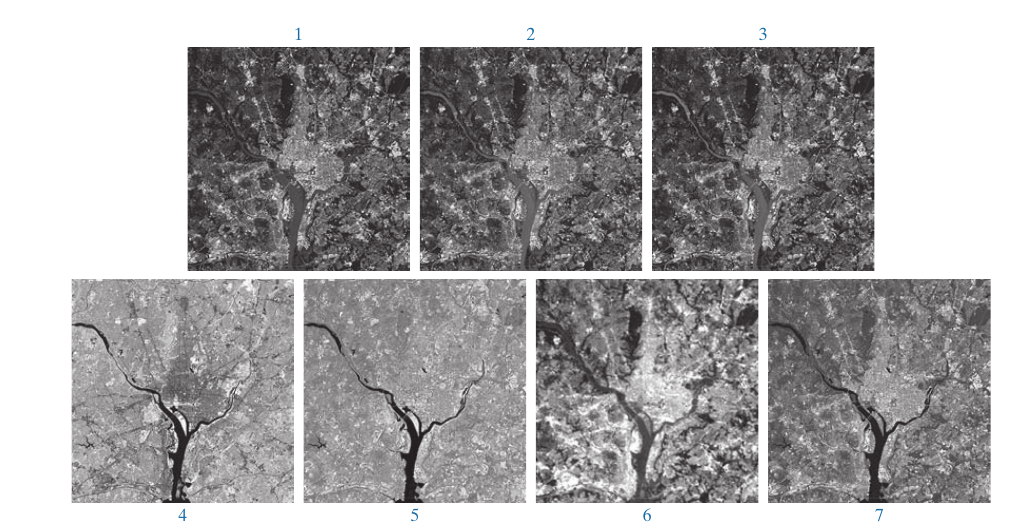
\includegraphics[width=0.8\textwidth]{src/assets/fundamentacao/landsat_bands.png}
    \captionsetup{justification=raggedright}
    \caption*{Fonte: \citefigure{gonzalez2018digital}}
    \label{fig:landsat_bands}
\end{figure}

Uma HSI tem alta resolução espectral, mas baixa resolução espacial \cite{Viel2019}, porque o sensor concentra a captura de cada ponto da cena em centenas de bandas estreitas e contíguas. A Figura \ref{fig:hsi_structure} mostra como o dado se forma: a plataforma do sensor, em movimento, captura linhas de varredura sucessivas, que são empilhadas em um hipercubo com duas dimensões espaciais e uma espectral.

\begin{figure}[H]
    \centering
    \captionsetup{justification=centering}
    \caption{Estrutura de dados de uma imagem hiperespectral: (a) aquisição por sensor em movimento; (b) formação do hipercubo tridimensional; (c) dimensões espaciais e canais espectrais}
    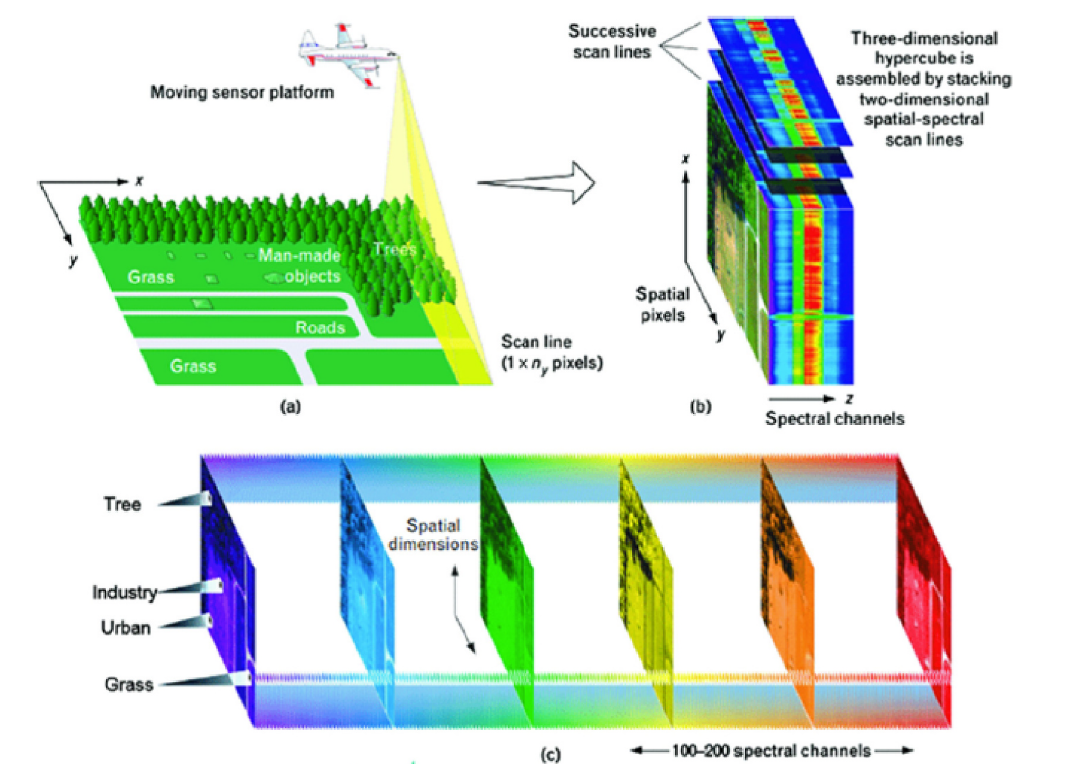
\includegraphics[width=0.75\textwidth]{src/assets/fundamentacao/hsi_structure.png}
    \captionsetup{justification=raggedright}
    \caption*{Fonte: \citefigure{Qian2020}}
    \label{fig:hsi_structure}
\end{figure}

A alta dimensionalidade das HSIs traz três desafios principais à sua análise: (1) a alta redundância de dados, causada pela forte correlação entre bandas espectrais adjacentes; (2) a variabilidade das assinaturas hiperespectrais, que podem mudar com as condições atmosféricas ou de iluminação; e (3) a maldição da dimensionalidade (\textit{curse of dimensionality}), em que o grande número de bandas prejudica o desempenho dos algoritmos de classificação e exige um número exponencialmente maior de amostras de treinamento \cite{Ahmad_2025}. As etapas básicas da análise de HSIs incluem pré-processamento, extração e seleção de características, e classificação ou desmistura (\textit{unmixing}) espectral.

\subsection{Redução de Dimensionalidade}

O número de bandas das HSIs e a correlação entre bandas adjacentes motivam a redução de dimensionalidade antes da classificação. A Análise de Componentes Principais (PCA) projeta os dados sobre as direções de maior variância e, com poucas componentes, preserva a maior parte da variância dos dados originais \cite{Jolliffe2002}. A projeção é definida pela equação:

\begin{equation}
z_i^t = w_i^T x^t, \quad i=1,\ldots,k, \quad t=1,\ldots,N
\end{equation}
\addEquacao{Projeção PCA}{6}

\noindent onde $x^t$ são os dados de entrada do pixel $t$, $w_i$ são os autovetores correspondentes aos maiores autovalores, $z_i^t$ são as componentes principais projetadas, $k$ é o número de componentes principais retidas, e $N$ é o número total de pixels. O algoritmo envolve: (1) centralização dos dados, subtraindo a média espectral; (2) cálculo da matriz de covariância; (3) decomposição da matriz de covariância em autovetores e autovalores; e (4) projeção dos dados originais nos autovetores correspondentes aos maiores autovalores \cite{Jolliffe2002}. Neste trabalho, o número $k$ de componentes retidas é um dos hiperparâmetros do espaço de busca (\autoref{qua:espaco}).

\section{Processamento de Imagens}

Uma imagem pode ser definida como uma função bidimensional, $f(x, y)$, onde $x$ e $y$ são coordenadas espaciais, e a amplitude de $f$ em qualquer par de coordenadas $(x, y)$ é chamada de intensidade ou nível de cinza da imagem naquele ponto \cite{gonzalez2018digital}. Quando $x$, $y$ e os valores de intensidade de $f$ são quantidades finitas e discretas, a imagem é chamada de imagem digital. O campo do processamento digital de imagens refere-se ao processamento de imagens digitais por meio de um computador digital.

O processamento de imagens pode ser categorizado em três níveis: baixo nível (pré-processamento, redução de ruído, realce de contraste), nível médio (segmentação, descrição de objetos, classificação) e alto nível (análise de cena e reconhecimento) \cite{gonzalez2018digital}. A Figura \ref{fig:erosion_example} exemplifica uma operação morfológica de erosão, um tipo de processamento de baixo nível comumente utilizado para remover componentes indesejados de imagens binárias.

\begin{figure}[H]
    \centering
    \captionsetup{justification=centering}
    \caption{Exemplo de operação de erosão morfológica aplicada a uma imagem binária usando elementos estruturantes de diferentes tamanhos}
    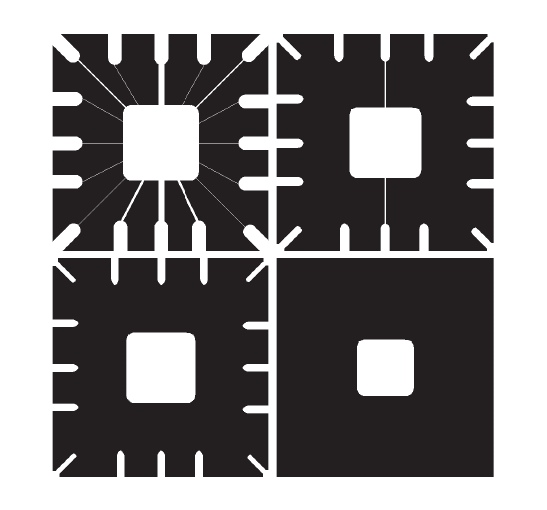
\includegraphics[width=0.55\textwidth]{src/assets/fundamentacao/erosion_example.png}
    \captionsetup{justification=raggedright}
    \caption*{Fonte: \citefigure{gonzalez2018digital}}
    \label{fig:erosion_example}
\end{figure}

A Figura \ref{fig:segmentation_cells} exemplifica o processamento de nível médio, mostrando a segmentação e identificação de células individuais em imagens microscópicas.

\begin{figure}[H]
    \centering
    \captionsetup{justification=centering}
    \caption{Exemplo de processamento de nível médio: segmentação de células em imagens microscópicas}
    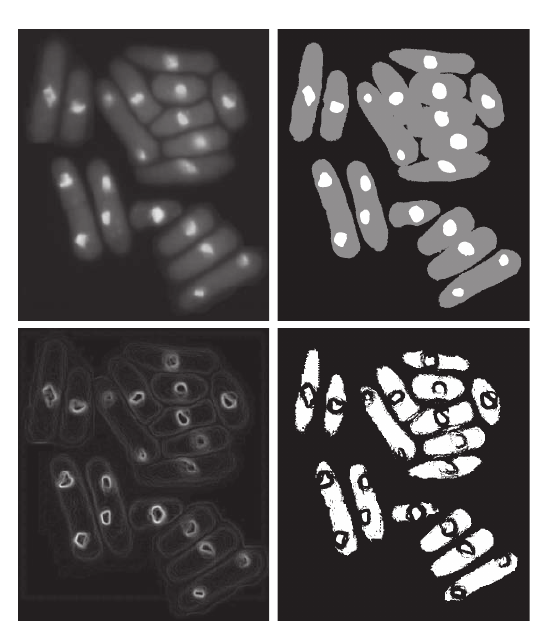
\includegraphics[width=0.5\textwidth]{src/assets/fundamentacao/segmentation_cells.png}
    \captionsetup{justification=raggedright}
    \caption*{Fonte: \citefigure{gonzalez2018digital}}
    \label{fig:segmentation_cells}
\end{figure}

A Figura \ref{fig:sift_matching} exemplifica o processamento de alto nível, mostrando o reconhecimento e correspondência de características entre imagens usando o algoritmo SIFT.

\begin{figure}[H]
    \centering
    \captionsetup{justification=centering}
    \caption{Exemplo de processamento de alto nível: correspondência de características usando SIFT, mostrando 41 pares encontrados com apenas 3 erros reais}
    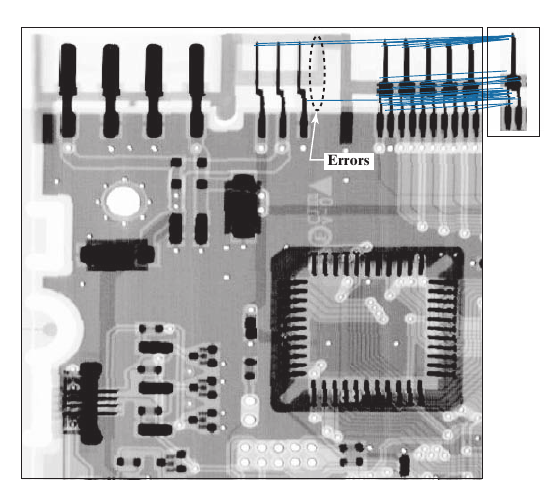
\includegraphics[width=0.55\textwidth]{src/assets/fundamentacao/sift_matching.png}
    \captionsetup{justification=raggedright}
    \caption*{Fonte: \citefigure{gonzalez2018digital}}
    \label{fig:sift_matching}
\end{figure}

\subsection{Segmentação de Imagens}
\label{subsec:fundSegmentacao}

No fluxo de classificação deste trabalho, a segmentação extrai a informação espacial que complementa as características espectrais. A segmentação de imagens é o processo de particionar uma imagem em múltiplos segmentos ou regiões de interesse \cite{FENG2019309}, e sua função é simplificar a representação da imagem em algo mais fácil de analisar. No domínio das HSIs, a segmentação usa a informação espacial para auxiliar a classificação, o que é útil quando objetos distintos apresentam assinaturas espectrais parecidas, mas estruturas geométricas ou texturas diferentes \cite{Souza2023}. Em Indian Pines, por exemplo, milho e soja aparecem cada um em três classes, conforme o manejo do solo; os espectros dessas classes diferem pouco entre si, mas cada uma ocupa talhões contíguos, e a região a que o pixel pertence pode ajudar a separar o que o espectro sozinho confunde. A Figura \ref{fig:segmentation_types} ilustra os dois principais tipos de mapa de segmentação gerados pelo algoritmo SEEDS: o mapa de bordas, que identifica os contornos entre superpixels, e o mapa de regiões, que atribui rótulos únicos a cada segmento homogêneo da imagem.

\begin{figure}[H]
    \centering
    \captionsetup{justification=centering}
    \caption{Tipos de mapa de segmentação: bordas (superior) e regiões (inferior) gerados pelo algoritmo SEEDS}
    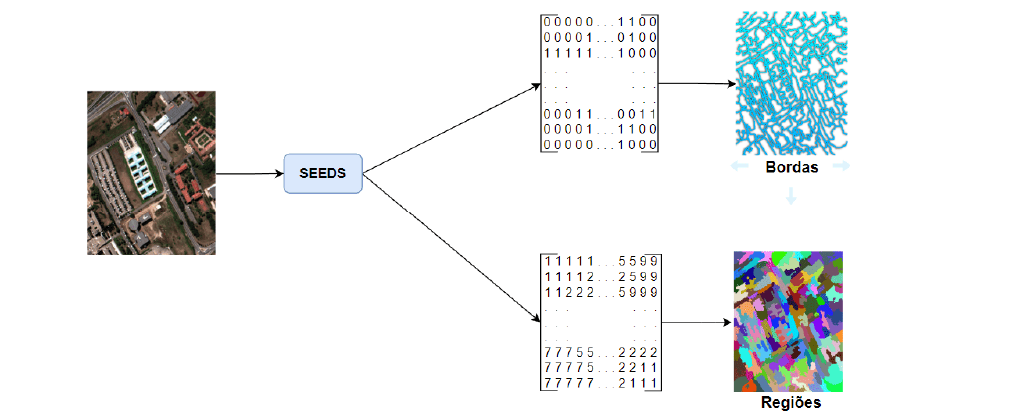
\includegraphics[width=0.85\textwidth]{src/assets/fundamentacao/segmentation_types.png}
    \captionsetup{justification=raggedright}
    \caption*{Fonte: \citefigure{Souza2023}}
    \label{fig:segmentation_types}
\end{figure}

Um método de segmentação morfológica utiliza os resíduos de transformadas de abertura e fechamento morfológicas baseadas em uma métrica geodésica \cite{Pesaresi905239}. Essa abordagem introduz o conceito de nivelamento (\textit{leveling}). A reconstrução em tons de cinza de uma imagem $g$ a partir de um marcador $f$ é obtida pelo uso iterativo de dilatações geodésicas elementares até a idempotência:

\begin{equation}
R_g^\delta(f) = \delta_g^{(i)}(f)
\end{equation}
\addEquacao{Reconstrução Geodésica Morfológica}{7}

\noindent onde $R_g^\delta(f)$ é a reconstrução geodésica do marcador $f$ sob a imagem de referência $g$, e $\delta_g^{(i)}(f)$ representa a dilatação geodésica elementar aplicada iterativamente até atingir idempotência (estabilidade). A característica morfológica multiescala de um ponto na imagem é definida pelo tamanho do elemento estruturante que possui o maior valor associado na derivada do perfil morfológico. O vetor da derivada do perfil morfológico (DMP) é:

\begin{equation}
\Delta(x) = (\Delta_0(x), ..., \Delta_\lambda(x), ..., \Delta_N(x))
\end{equation}
\addEquacao{Vetor de Derivada do Perfil Morfológico (DMP)}{8}

\noindent onde $\Delta(x)$ é o vetor de derivadas do perfil morfológico no ponto $x$, $\Delta_\lambda(x)$ representa a derivada para o elemento estruturante de tamanho $\lambda$, e $N$ é o número total de escalas.

O SEEDS (\textit{Superpixels Extracted via Energy-Driven Sampling}) parte de uma partição da imagem em grade regular e refina as fronteiras dos superpixels por \textit{hill-climbing}: blocos de pixels, e depois pixels isolados, passam para um superpixel vizinho sempre que a troca aumenta uma função de energia \cite{bergh2013seedssuperpixelsextractedenergydriven}:

\begin{equation}
E(s) = H(s) + \gamma G(s)
\end{equation}
\addEquacao{Função de Energia do Algoritmo SEEDS}{9}

\noindent onde $E(s)$ é a energia da segmentação $s$, $H(s)$ é o termo de histograma, que mede a homogeneidade de cor dentro de cada superpixel, $G(s)$ é o termo de contorno, que favorece fronteiras suaves, e $\gamma$ controla o equilíbrio entre cor e contornos.

Além do SEEDS, três outros algoritmos de superpixels são usados neste trabalho. O SLIC (\textit{Simple Linear Iterative Clustering}) distribui sementes em uma grade regular de espaçamento $S$ e executa um \textit{k-means} local, em que cada pixel é atribuído à semente mais próxima segundo uma distância que combina cor e posição; a busca de cada semente fica restrita a uma janela de $2S \times 2S$ ao seu redor \cite{Achanta2012SLIC}. A variante SLICO ajusta a compacidade automaticamente, dispensando o parâmetro que a controla. O LSC (\textit{Linear Spectral Clustering}) mapeia cada pixel para um espaço de características de dimensão mais alta, no qual um \textit{k-means} ponderado aproxima o critério de cortes normalizados em grafos, o que tende a produzir bordas mais aderentes aos contornos da imagem \cite{Zhengqin7298741}. O Watershed trata a magnitude do gradiente como um relevo topográfico e o inunda a partir de marcadores; as fronteiras entre regiões surgem onde águas de bacias diferentes se encontram \cite{Najman546254}. Todos eles, assim como o SEEDS, recebem como entrada uma imagem de três canais: no caso das HSIs, uma composição das três primeiras componentes principais.

\subsection{Métricas de Avaliação}

As métricas de classificação de HSIs derivam da matriz de confusão, que cruza, para cada pixel avaliado, a classe verdadeira com a classe prevista \cite{Congalton1991}. Sejam $n_{ij}$ o número de pixels da classe verdadeira $i$ atribuídos à classe $j$, $c$ o número de classes, $N$ o total de pixels avaliados, e $n_{i+} = \sum_{j} n_{ij}$ e $n_{+i} = \sum_{j} n_{ji}$ os totais da linha e da coluna da classe $i$. As três métricas usadas neste trabalho são as seguintes.

\textbf{Acurácia Geral (Overall Accuracy - OA):}

\begin{equation}
OA = \frac{1}{N} \sum_{i=1}^{c} n_{ii}
\end{equation}
\addEquacao{Acurácia Geral (OA)}{10}

\noindent isto é, a proporção de pixels classificados corretamente \cite{Congalton1991}. Com duas classes, a expressão se reduz a $(vp + vn)/(vp + vn + fp + fn)$, em que $vp$, $vn$, $fp$ e $fn$ são os verdadeiros positivos, os verdadeiros negativos, os falsos positivos e os falsos negativos.

\textbf{Acurácia Média (Average Accuracy - AA):}

\begin{equation}
AA = \frac{1}{c} \sum_{i=1}^{c} \frac{n_{ii}}{n_{i+}}
\end{equation}
\addEquacao{Acurácia Média (AA)}{11}

\noindent onde $n_{ii}/n_{i+}$ é a acurácia da classe $i$, isto é, a fração dos seus pixels classificada corretamente. Como cada classe pesa o mesmo, a AA pune o classificador que acerta só as classes grandes. Por exemplo, um classificador que acerta 85 dos 90 pixels de uma classe frequente, mas só 4 dos 10 pixels de uma classe rara e 8 dos 10 de outra, tem OA de 0,88 e AA de 0,71. Em Indian Pines, cujas classes vão de 20 a 2.455 pixels rotulados, a distância entre as duas métricas é grande.

\textbf{Coeficiente Kappa ($\kappa$):}

\begin{equation}
\kappa = \frac{p_o - p_e}{1 - p_e}
\end{equation}
\addEquacao{Coeficiente Kappa}{12}

\noindent onde $p_o$ é a concordância observada, igual à OA, e $p_e = \frac{1}{N^2} \sum_{i=1}^{c} n_{i+}\, n_{+i}$ é a concordância esperada por acaso, calculada pelos totais de linha e de coluna. Proposto por \citeonline{Cohen1960}, o coeficiente mede a concordância entre a classificação e o Ground Truth (GT) descontando a parcela que ocorreria por acaso: vale 1 para concordância perfeita e 0 quando a concordância é a esperada por acaso \cite{Congalton1991}.

\section{Aprendizado de Máquina}

O Aprendizado de Máquina, do inglês \textit{Machine Learning} (ML), é o campo de estudo que dá aos computadores a capacidade de aprender sem serem explicitamente programados \cite{SomeStudiesinMachineLearningUsingtheGameofCheckers}. O aprendizado profundo, ao qual pertencem as CNNs usadas neste trabalho, é um de seus ramos \cite{DeeplearningLC}. Um programa de computador aprende a partir de uma experiência ($E$) com respeito a uma classe de tarefas ($T$) e uma medida de desempenho ($P$) se o seu desempenho nas tarefas em $T$, medido por $P$, melhora com a experiência $E$ \cite{MachineLearning}. A Figura \ref{fig:checkers_tree} mostra um exemplo clássico, o programa de damas de \citeonline{SomeStudiesinMachineLearningUsingtheGameofCheckers}, que avalia os movimentos possíveis por meio de uma árvore de jogadas e escolhe o ramo de maior pontuação.

\begin{figure}[H]
    \centering
    \captionsetup{justification=centering}
    \caption{Diagrama simplificado mostrando como as avaliações são respaldadas através da árvore de movimentos possíveis para chegar ao melhor próximo movimento}
    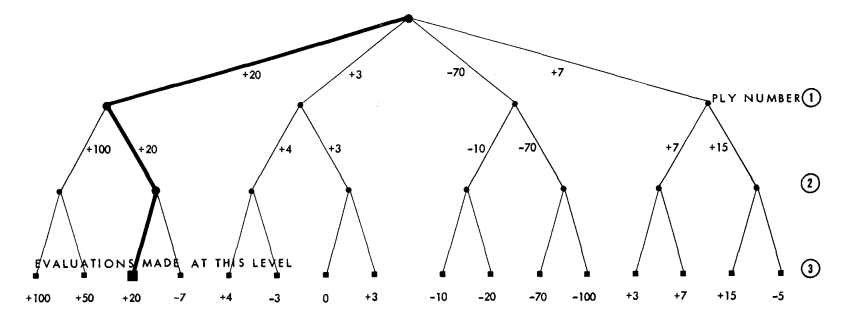
\includegraphics[width=0.75\textwidth]{src/assets/fundamentacao/checkers_tree.png}
    \captionsetup{justification=raggedright}
    \caption*{Fonte: \citefigure{SomeStudiesinMachineLearningUsingtheGameofCheckers}}
    \label{fig:checkers_tree}
\end{figure}

\subsection{Desafios Centrais: Generalização e Sobreajuste}

O desafio principal é garantir que o desempenho de um modelo ($P$) melhore não apenas nos dados de treinamento ($E$), mas também em dados novos. Quando isso não ocorre, há sobreajuste, do inglês \textit{overfitting} (OF): o modelo se ajusta demais aos dados de treinamento e captura ruído em vez do padrão subjacente \cite{Overfittingproblem:anewperspectivefromthegeometricalinterpretationofMLP}, com bom desempenho no treinamento e desempenho ruim em entradas novas. Por isso o desempenho é acompanhado em um conjunto de validação, separado do treino. A Figura \ref{fig:gradient_descent} traz um exemplo de \citeonline{DeepLearningIG}: durante o treino de uma rede convolucional, a norma do gradiente cresce, sinal de que o otimizador não chega a um ponto crítico, e ainda assim o erro de classificação na validação cai a um nível baixo. O que indica se o modelo generaliza é esse erro, medido fora do treino, e não a convergência do otimizador.

As estratégias de regularização restringem a complexidade efetiva do modelo para reduzir o OF \cite{DeepLearningIG}. Três delas aparecem neste trabalho: o \textit{dropout}, que desativa ao acaso uma fração dos neurônios a cada passo de treino e impede que eles se coadaptem \cite{Dropout:asimplewaytopreventneuralnetworksfromoverfitting}, usado nas duas camadas densas ocultas da rede; o \textit{weight decay}, que penaliza a norma dos pesos; e a parada antecipada, que interrompe o treino quando o desempenho na validação deixa de melhorar \cite{DeepLearningIG}.

\begin{figure}[H]
    \centering
    \captionsetup{justification=centering}
    \caption{Comportamento da descida de gradiente durante o treinamento de uma rede convolucional: (Esquerda) distribuição das normas do gradiente ao longo do tempo; (Direita) taxa de erro de classificação no conjunto de validação}
    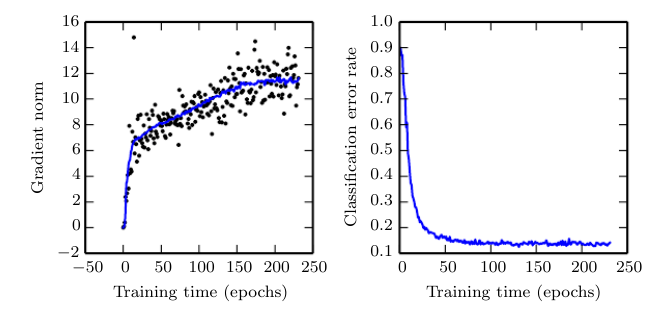
\includegraphics[width=0.85\textwidth]{src/assets/fundamentacao/gradient_descent_behavior.png}
    \captionsetup{justification=raggedright}
    \caption*{Fonte: \citefigure{DeepLearningIG}}
    \label{fig:gradient_descent}
\end{figure}

\subsection{Paradigmas de Aprendizagem}

A natureza dos dados e do problema determina qual paradigma de aprendizado usar \cite{WhatIsMachineLearning}. A Figura \ref{fig:learning_paradigms} ilustra os três principais paradigmas e a relação de cada um com o tipo de dado de treinamento.

\begin{figure}[H]
    \centering
    \captionsetup{justification=centering}
    \caption{Paradigmas de aprendizagem e sua relação com os tipos de dados de treinamento}
    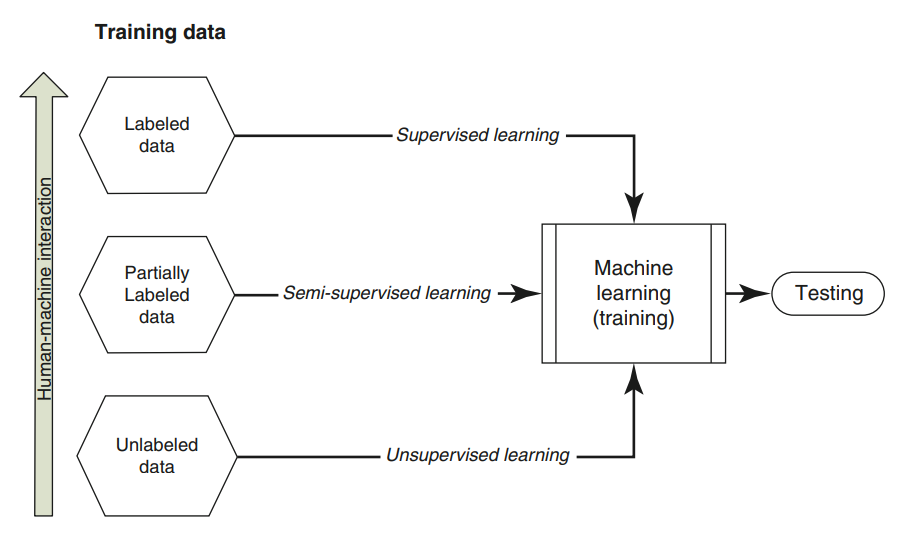
\includegraphics[width=0.65\textwidth]{src/assets/fundamentacao/learning_paradigms.png}
    \captionsetup{justification=raggedright}
    \caption*{Fonte: \citefigure{WhatIsMachineLearning}}
    \label{fig:learning_paradigms}
\end{figure}

\begin{itemize}
    \item \textbf{Aprendizado Supervisionado}: Estima um mapeamento a partir de amostras de entrada e saída, em que as saídas são rótulos ou valores conhecidos. As tarefas mais comuns são classificação e regressão. É o paradigma deste trabalho: cada pixel rotulado do GT fornece um espectro de entrada e a classe esperada.

    \item \textbf{Aprendizado Não Supervisionado}: O sistema recebe apenas amostras de entrada, sem rótulos, e procura estrutura nos próprios dados, como grupos de amostras semelhantes. Os algoritmos de superpixels SLIC e LSC (\autoref{subsec:fundSegmentacao}) são exemplos: agrupam pixels por \textit{k-means} sem usar nenhum rótulo.

    \item \textbf{Aprendizado Semissupervisionado}: Do inglês \textit{Semi-supervised learning} (SSL), situa-se entre os dois paradigmas anteriores e usa dados em que apenas parte das amostras é rotulada.
\end{itemize}

\subsection{Aprendizado Profundo}

Os sistemas tradicionais de reconhecimento de padrões eram formados por dois módulos: um extrator de características projetado manualmente e um classificador treinável, e o desempenho dependia da engenharia dessas características \cite{DeeplearningLC}. O Aprendizado Profundo, do inglês \textit{Deep Learning} (DL), remove essa dependência: modelos compostos por múltiplas camadas de processamento aprendem, diretamente dos dados brutos, representações com múltiplos níveis de abstração \cite{Asurveyonstate-of-the-artdeeplearningapplicationsandchallenges}. O DL é um método de aprendizado de representação obtido pela composição de módulos simples e não lineares, em que cada camada transforma a representação da camada anterior em uma de nível de abstração superior \cite{DeeplearningLC}. A Figura \ref{fig:cnn_architecture} ilustra a arquitetura de uma rede neural convolucional, com convoluções seguidas da função de ativação ReLU e camadas de \textit{max pooling} que reduzem progressivamente a dimensão espacial. As funções de ativação, como a Unidade Linear Retificada (ReLU), introduzem não linearidades na rede. A ReLU é definida como:

\begin{equation}
f(z) = \max(z, 0) = \begin{cases} 
z, & \text{se } z > 0 \\
0, & \text{caso contrário}
\end{cases}
\end{equation}
\addEquacao{Função de Ativação ReLU}{1}

\noindent onde $z$ é a entrada da função de ativação. Por não saturar para entradas positivas, a ReLU acelera o treino em relação a funções saturantes, como a sigmoide e a tangente hiperbólica: em uma rede convolucional de quatro camadas treinada no CIFAR-10, a versão com ReLU atingiu 25\% de erro de treino seis vezes mais rápido que a versão com tangente hiperbólica \cite{NIPS2012_c399862d}. O treinamento dessas redes usa o algoritmo de retropropagação, do inglês \textit{backpropagation}, que calcula o gradiente da função de perda em relação a cada peso da rede e permite ajustar os parâmetros por descida de gradiente \cite{Gradient-basedlearningappliedtodocumentrecognition}. A Figura \ref{fig:backpropagation} mostra como uma rede neural multicamadas pode distorcer o espaço de entrada para tornar as classes linearmente separáveis, e como a retropropagação aplica a regra da cadeia, tanto na propagação para frente (\textit{forward pass}) quanto na retropropagação dos gradientes (\textit{backward pass}).

\begin{figure}[H]
    \centering
    \captionsetup{justification=centering}
    \caption{Redes neurais multicamadas e backpropagation: (a) transformação do espaço de entrada; (b) regra da cadeia; (c) equações do forward pass; (d) equações do backward pass}
    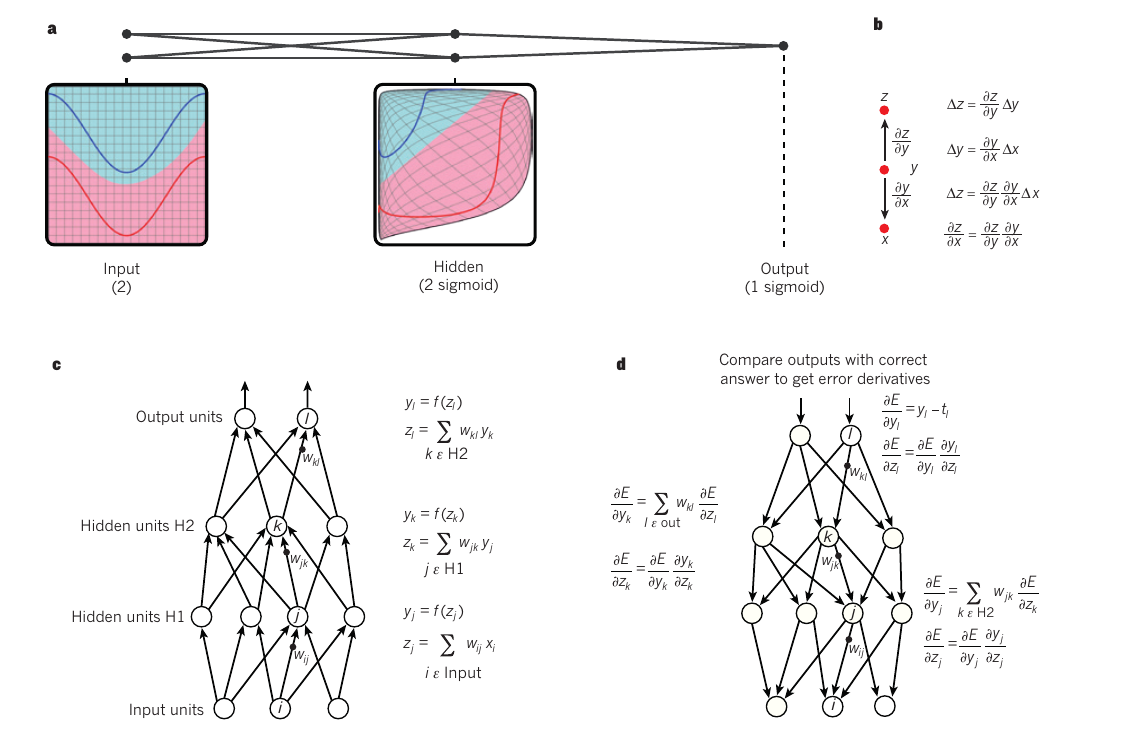
\includegraphics[width=0.75\textwidth]{src/assets/fundamentacao/backpropagation.png}
    \captionsetup{justification=raggedright}
    \caption*{Fonte: \citefigure{DeeplearningLC}}
    \label{fig:backpropagation}
\end{figure}

\begin{figure}[H]
    \centering
    \captionsetup{justification=centering}
    \caption{Arquitetura de uma rede neural convolucional mostrando camadas de convolução com ReLU e max pooling}
    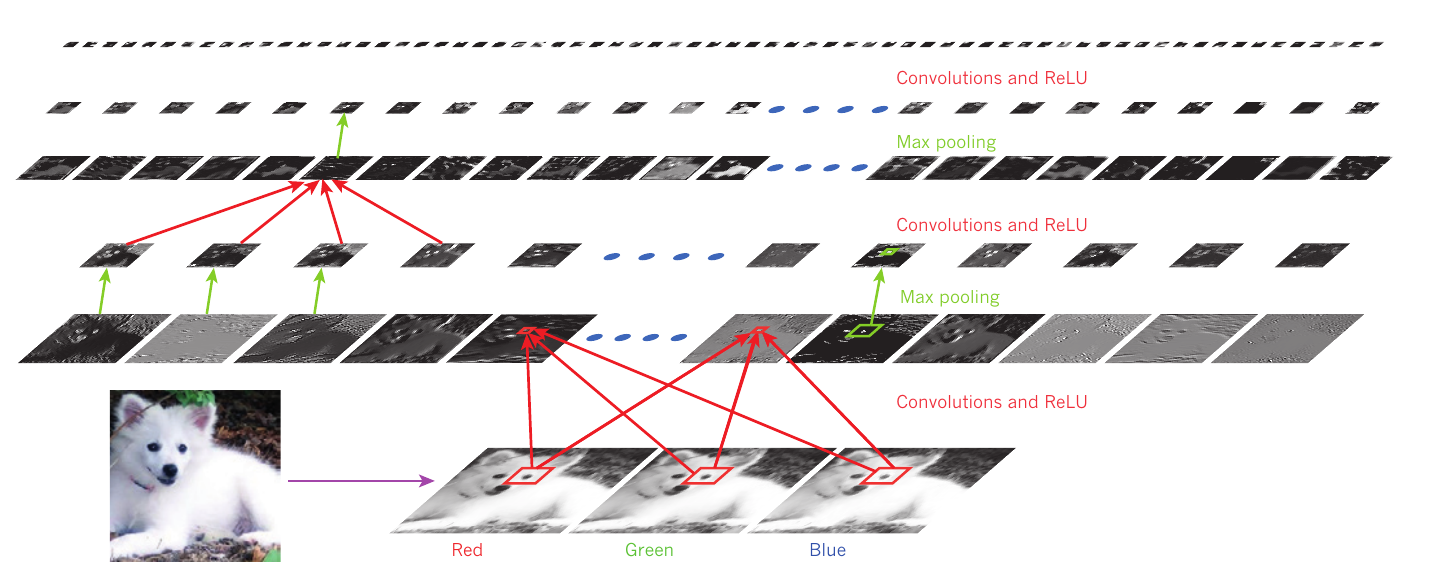
\includegraphics[width=0.9\textwidth]{src/assets/fundamentacao/cnn_architecture.png}
    \captionsetup{justification=raggedright}
    \caption*{Fonte: \citefigure{DeeplearningLC}}
    \label{fig:cnn_architecture}
\end{figure}

O treinamento de redes neurais profundas usa algoritmos de otimização estocástica para ajustar os parâmetros do modelo; o Adam, usado neste trabalho, é um deles \cite{kingma2017adammethodstochasticoptimization}. O gradiente é definido como:

\begin{equation}
\nabla_{\theta} L = \frac{\partial L}{\partial \theta}
\end{equation}
\addEquacao{Gradiente da Função de Perda}{2}

\noindent onde $\nabla_{\theta}$ é o operador gradiente, $L$ é a função de perda, e $\theta$ são os parâmetros do modelo. A função de perda depende da tarefa: em regressão, a escolha usual é o erro quadrático médio; em classificação, como neste trabalho (\autoref{subsec:desTreino}), usa-se a entropia cruzada \cite{DeepLearningIG}:

\begin{equation}
L = -\frac{1}{N} \sum_{t=1}^{N} \sum_{i=1}^{c} r_i^t \log y_i^t
\end{equation}
\addEquacao{Entropia Cruzada}{3}

\noindent onde $N$ é o número de amostras, $c$ é o número de classes, $r_i^t$ vale 1 se a amostra $t$ pertence à classe $i$ e 0 caso contrário, e $y_i^t$ é a probabilidade da classe $i$ prevista pelo modelo para a entrada $x^t$, obtida pela função \textit{softmax} aplicada à saída da última camada.

\subsubsection{Redes Neurais Convolucionais}

As CNNs são um tipo especializado de rede neural projetado para processar dados com topologia de grade \cite{DeepLearningIG}, como o espectro de um pixel, que é uma grade unidimensional. Sua arquitetura se apoia em quatro ideias: conexões locais, pesos compartilhados, agrupamento (\textit{pooling}) e uso de múltiplas camadas \cite{DeeplearningLC}. A operação de convolução em uma dimensão (1D) é definida como:

\begin{equation}
s(t) = (x \ast w)(t) = \sum_{a=-\infty}^{\infty} x(a) \cdot w(t-a)
\end{equation}
\addEquacao{Operação de Convolução 1D}{4}

\noindent onde $x$ é o sinal de entrada, $w$ é o \textit{kernel} (filtro) da convolução e $s(t)$ é o resultado da operação na posição $t$. Na CNN 1D deste trabalho, o sinal de entrada é o espectro de um pixel após o PCA, e $t$ percorre as componentes espectrais. A Figura \ref{fig:convolution_operation} mostra, no caso bidimensional, o \textit{kernel} aplicado sobre a matriz de entrada.

\begin{figure}[H]
    \centering
    \captionsetup{justification=centering}
    \caption{Operação de convolução mostrando a aplicação do kernel sobre a matriz de entrada}
    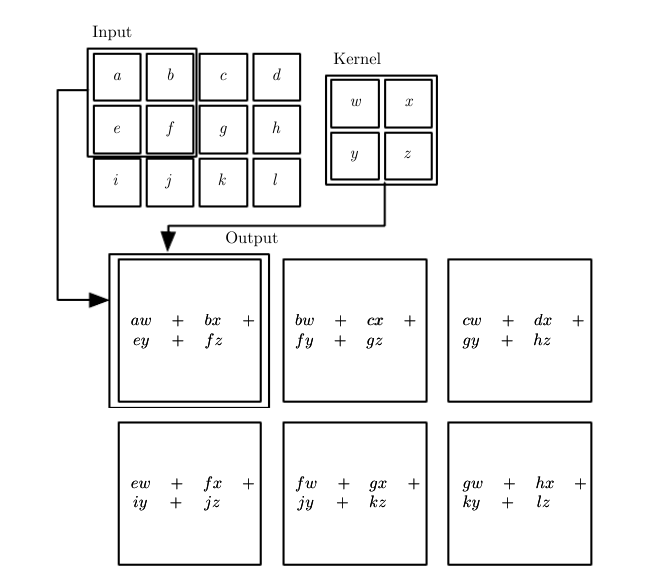
\includegraphics[width=0.6\textwidth]{src/assets/fundamentacao/convolution_operation.png}
    \captionsetup{justification=raggedright}
    \caption*{Fonte: \citefigure{DeeplearningLC}}
    \label{fig:convolution_operation}
\end{figure}

\noindent Em vez de conectar cada neurônio de uma camada a todos os neurônios da camada anterior, os neurônios em uma camada convolucional são conectados apenas a uma região local (conexões locais) \cite{DeeplearningLC}. A entrada líquida (\textit{net input}) em um neurônio convolucional é:

\begin{equation}
z_{x,y}^{\ell} = b^{\ell} + \sum_{l,k} w_{l,k}^{\ell} \cdot a_{x-l,y-k}^{\ell-1}
\end{equation}
\addEquacao{Entrada Líquida em Camada Convolucional}{5}

\noindent onde $z_{x,y}^{\ell}$ é a entrada na posição $(x,y)$ da camada $\ell$, $b^{\ell}$ é o viés (\textit{bias}), $w_{l,k}^{\ell}$ são os pesos do \textit{kernel} e $a_{x-l,y-k}^{\ell-1}$ são as ativações da camada anterior. Todas as unidades de um mesmo mapa de características compartilham o mesmo conjunto de pesos, o que reduz o número de parâmetros. Essa abordagem assume que um detector de características útil em uma parte da imagem será útil em outra parte. A camada de \textit{pooling} reduz a dimensão espacial dos mapas de características e torna a representação mais compacta e robusta a pequenas translações. Uma CNN típica consiste em estágios de camadas convolucionais seguidas por camadas de \textit{pooling}, e termina em camadas totalmente conectadas para a classificação.

Na convolução, cada elemento do mapa de características de saída depende apenas de uma região local da entrada e dos pesos do \textit{kernel} compartilhado, e não dos demais elementos da mesma camada. Essa independência de dados entre elementos de saída é o que permite calcular a camada em paralelo na GPU (\autoref{sec:paralelismo}).

A evolução das arquiteturas de CNNs é marcada pelo aumento progressivo da profundidade. Redes pioneiras como a LeNet-5 demonstraram a eficácia da combinação de camadas convolucionais e de \textit{pooling} no reconhecimento de caracteres \cite{Gradient-basedlearningappliedtodocumentrecognition}. A VGG mostrou que redes profundas podiam ser construídas com filtros pequenos ($3 \times 3$) \cite{VeryDeepConvolutionalNetworksforLarge-ScaleImageRecognition}. A GoogLeNet introduziu os módulos \textit{Inception}, que executam convoluções de diferentes tamanhos em paralelo \cite{szegedy2014goingdeeperconvolutions}.

\subsubsection{Aplicações de CNNs}

As CNNs são usadas em várias aplicações:

\begin{itemize}
    \item \textbf{Classificação de Imagens}: Atribui um único rótulo a uma imagem inteira \cite{NIPS2012_c399862d}.

    \item \textbf{Segmentação Semântica}: Classifica cada pixel de uma imagem em uma categoria específica \cite{Farabet6338939}. Em sensoriamento remoto, é usada no mapeamento de cobertura do solo \cite{rs16152729}.

    \item \textbf{Detecção de Objetos}: Localiza múltiplos objetos em uma imagem por meio de caixas delimitadoras (\textit{bounding boxes}) e classifica cada um \cite{sermanet2014overfeatintegratedrecognitionlocalization}.

    \item \textbf{Análise de Imagens Hiperespectrais}: Em imagens hiperespectrais, que contêm centenas de bandas espectrais, as CNNs extraem características espectrais e espaciais \cite{Li2019DeepLF}. A Figura \ref{fig:cnn1d_hsi} ilustra uma arquitetura CNN 1D para classificação de HSIs, do pré-processamento por PCA às camadas convolucionais 1D e densas que produzem a classificação.
\end{itemize}

\begin{figure}[H]
    \centering
    \captionsetup{justification=centering}
    \caption{Arquitetura CNN 1D para classificação de imagens hiperespectrais: pré-processamento PCA seguido de 4 camadas convolucionais 1D e camadas densas para classificação}
    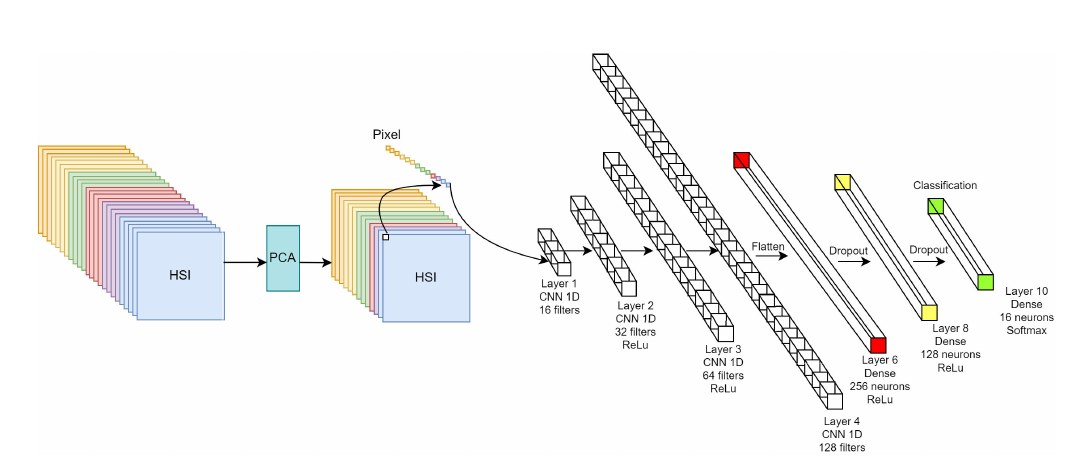
\includegraphics[width=0.95\textwidth]{src/assets/fundamentacao/cnn1d_hsi_architecture.png}
    \captionsetup{justification=raggedright}
    \caption*{Fonte: \citefigure{Viel10064297}}
    \label{fig:cnn1d_hsi}
\end{figure}

\section{Processamento Paralelo em GPUs}
\label{sec:paralelismo}

Neste trabalho, a CNN é treinada em GPU, exceto nas medições de paralelismo, feitas em CPU (\autoref{sec:resParalelismo}), e a segmentação é sempre executada em CPU. A arquitetura da GPU e o modelo de programação CUDA explicam por que as convoluções da rede se paralelizam bem, e a independência entre as etapas do fluxo define as demais estratégias de paralelização.

\subsection{Arquitetura de GPUs e CUDA Cores}

As Unidades de Processamento Gráfico (GPUs) evoluíram de aceleradores gráficos especializados para processadores paralelos de propósito geral \cite{CUDA_Programming}. Enquanto uma CPU tem tipicamente dezenas de núcleos otimizados para execução sequencial com baixa latência, uma GPU NVIDIA tem milhares de núcleos de processamento mais simples, os \textit{CUDA cores}, organizados em unidades chamadas \textit{Streaming Multiprocessors} (SMs) \cite{CUDA_Programming}.

Cada \textit{CUDA core} executa operações aritméticas de ponto flutuante, como soma, multiplicação e a operação fusionada de multiplicação e soma (FMA). Os \textit{CUDA cores} de um SM seguem o modelo SIMT (\textit{Single Instruction, Multiple Threads}): grupos de 32 threads, chamados \textit{warps}, executam a mesma instrução ao mesmo tempo sobre dados diferentes \cite{CUDA_Programming}. Essa arquitetura é eficiente para operações com paralelismo de dados, em que a mesma operação é aplicada a muitos elementos independentes.

A plataforma CUDA (\textit{Compute Unified Device Architecture}), desenvolvida pela NVIDIA, fornece um modelo de programação que permite explorar o paralelismo das GPUs em aplicações de computação geral \cite{CUDA_Programming}. O modelo de execução organiza as threads em três níveis: threads individuais são agrupadas em blocos, e os blocos, em grades. Como o hardware distribui os blocos entre os SMs disponíveis, o mesmo programa se adapta a GPUs com números diferentes de SMs \cite{CUDA_Architecture}.

\subsection{Paralelização de Operações de Convolução}

A operação de convolução em CNNs apresenta características intrínsecas que a tornam altamente paralelizável \cite{cuConv}. Para uma camada convolucional com entrada $X$ de dimensões $(N, C_{in}, H, W)$ (lote, canais de entrada, altura, largura), filtros $K$ de dimensões $(C_{out}, C_{in}, k_h, k_w)$ e saída $Y$ de dimensões $(N, C_{out}, H_{out}, W_{out})$, cada elemento de saída é calculado como:

\begin{equation}
Y[n, c_{out}, i, j] = \sum_{c_{in}=0}^{C_{in}-1} \sum_{m=0}^{k_h-1} \sum_{l=0}^{k_w-1} X[n, c_{in}, i+m, j+l] \cdot K[c_{out}, c_{in}, m, l] + b[c_{out}]
\end{equation}

Nenhum elemento $Y[n, c_{out}, i, j]$ depende do cálculo de outro elemento da saída; os $N \times C_{out} \times H_{out} \times W_{out}$ elementos podem, portanto, ser calculados simultaneamente, se houver recursos computacionais suficientes. Na CNN 1D, a dimensão da altura desaparece e a propriedade se mantém: cada posição do mapa de características ao longo do espectro pode ser calculada em paralelo.

Na prática, \textit{frameworks} de aprendizado profundo como TensorFlow e PyTorch usam a biblioteca cuDNN da NVIDIA, que escolhe, para cada configuração da camada, um entre vários algoritmos de convolução \cite{Jorda_cuDNN}.

\subsection{Estratégias de Paralelização para o Fluxo de Classificação}

O treinamento e a inferência de CNNs admitem paralelismo em mais de um nível \cite{Aach2025, Nandan10910577}. Os três a seguir são os relevantes para o fluxo de classificação de HSIs.

\textbf{Paralelismo de Dados}: Réplicas do modelo processam subconjuntos diferentes dos dados ao mesmo tempo, e os gradientes são agregados para atualizar os pesos. A MirroredStrategy do TensorFlow e a DataParallel do PyTorch implementam essa estratégia, mais útil quando o conjunto de dados é grande e há várias GPUs disponíveis \cite{Nandan10910577}. A partição da cena, uma das estratégias deste trabalho, também divide os dados entre unidades de execução, mas sem agregar gradientes: cada parte da cena é processada por uma thread ou por um processo (\autoref{sec:desParalelismo}).

\textbf{Paralelismo Intra-Camada}: Dentro de uma camada convolucional, os elementos de saída são calculados em paralelo nos \textit{CUDA cores}. As implementações em GPU, como a cuDNN, exploram esse paralelismo automaticamente, sem intervenção do programador.

\textbf{Paralelismo entre Etapas}: Etapas que não dependem uma da outra podem ser executadas concorrentemente. No fluxo de \citeonline{Souza2023}, isso ocorre em dois pontos. Na preparação dos dados, o ramo espectral, que reduz o espectro por PCA, e o ramo espacial, que compõe as três primeiras componentes principais e segmenta a imagem, partem da mesma cena e só se reúnem na montagem das entradas da rede. Na inferência, a segmentação, executada em CPU pelo OpenCV, e as convoluções da rede também são independentes: as convoluções não usam o mapa de segmentação, e a sincronização só é necessária na concatenação, que precisa do identificador do superpixel de cada pixel. Essas duas oportunidades correspondem, neste trabalho, ao paralelismo entre os ramos do pré-processamento e à fusão concorrente (\autoref{sec:desParalelismo}); a biblioteca padrão do Python oferece threads e processos para executá-las \cite{Python_Threading}.

\section{Concorrência em CPU}
\label{sec:concorrencia}

O paralelismo entre etapas exige os conceitos clássicos de concorrência dos sistemas operacionais. Na fusão espectral-espacial, a segmentação, executada em CPU pelo OpenCV, e as convoluções da rede só se encontram no ponto de fusão.

\subsection{Threads, Processos e o GIL}

Um processo é um programa em execução com espaço de endereçamento próprio; uma thread é um fluxo de execução dentro de um processo, e as threads de um mesmo processo compartilham sua memória \cite{Silberschatz2018}. Criar uma thread é barato e não copia dados; processos são isolados, e trocar dados entre eles exige serializá-los e copiá-los, com custo proporcional ao volume transferido.

No CPython, o interpretador de referência do Python, o \textit{Global Interpreter Lock} (GIL) garante que apenas uma thread execute \textit{bytecode} Python por vez \cite{PEP703}. Código Python puro em várias threads, portanto, não executa em paralelo, enquanto código nativo que libera o GIL durante o cálculo, como as rotinas do NumPy, o OpenCV e os \textit{kernels} do PyTorch, executa (\autoref{fig:gil}). O ganho das threads depende da fração do trabalho que acontece fora do interpretador.

\begin{figure}[H]
    \centering
    \captionsetup{justification=centering}
    \caption{Quatro threads de um processo executando código Python e código nativo que libera o GIL}
    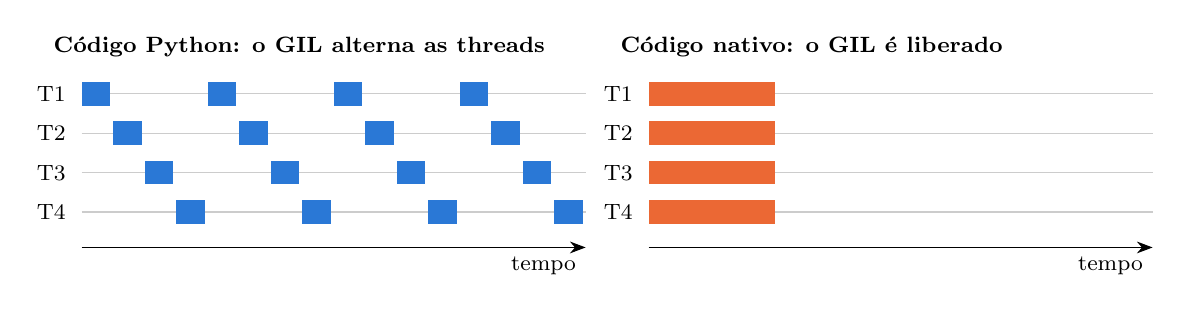
\begin{tikzpicture}[font=\footnotesize, x=0.8cm, y=0.5cm]
        \foreach \dx/\titulo in {0/{Código Python: o GIL alterna as threads}, 9/{Código nativo: o GIL é liberado}} {
            \node[anchor=south west, font=\footnotesize\bfseries] at (\dx-0.6, 3.7) {\titulo};
            \foreach \i in {1,...,4} {
                \node[anchor=east] at (\dx-0.1, 4-\i) {T\i};
                \draw[black!20] (\dx, 4-\i) -- (\dx+8, 4-\i);
            }
            \draw[-{Stealth[length=2mm]}] (\dx, -0.9) -- (\dx+8, -0.9) node[below left] {tempo};
        }
        \foreach \k in {0,...,15} {
            \pgfmathtruncatemacro{\linha}{mod(\k,4)+1}
            \fill[azulfig] ({0.5*\k}, {4-\linha-0.3}) rectangle ++(0.45, 0.6);
        }
        \foreach \i in {1,...,4} {
            \fill[laranjafig] (9, {4-\i-0.3}) rectangle ++(2.0, 0.6);
        }
    \end{tikzpicture}
    \captionsetup{justification=raggedright}
    \caption*{Fonte: Elaborada pelo autor}
    \label{fig:gil}
\end{figure}

\subsection{Exclusão Mútua e Variáveis de Condição}

Quando duas threads acessam o mesmo dado e ao menos uma o modifica, o resultado pode depender da ordem de execução, situação chamada de condição de corrida. O trecho que acessa o dado compartilhado é a seção crítica, protegida em geral por um mutex (de \textit{mutual exclusion}): uma trava que só uma thread detém por vez \cite{Silberschatz2018}. O mutex garante exclusão, mas não ordem: se a thread consumidora adquirir a trava antes da produtora, lerá o dado ainda não produzido. Para impor ordem, usa-se uma variável de condição, associada ao mutex e a um predicado: a consumidora verifica o predicado e, se ele for falso, espera com a trava liberada, até que a produtora atualize o dado e a notifique. Esse conjunto corresponde ao conceito de monitor \cite{Hoare1974Monitors}. A barreira, outra primitiva usada neste trabalho, bloqueia um grupo de threads até que todas cheguem ao mesmo ponto.

\subsection{Lei de Amdahl e \textit{Speedup}}

O \textit{speedup} é a razão entre o tempo de uma versão de referência e o da versão paralela, e a escolha da referência é parte da medição: comparar uma versão paralela em CPU com uma sequencial em GPU mede também a diferença de dispositivo. Pela lei de Amdahl \cite{Amdahl1967}, se uma fração $p$ do tempo de execução pode ser dividida entre $N$ unidades, o \textit{speedup} máximo é:

\begin{equation}
S(N) = \frac{1}{(1 - p) + \dfrac{p}{N}}
\end{equation}
\addEquacao{Lei de Amdahl}{13}

\noindent Dois corolários orientam este trabalho. Paralelizar uma etapa que responde por 1\% do tempo total muda esse tempo em no máximo 1\%. E, quando duas etapas independentes de durações $T_1$ e $T_2$ passam a ser executadas concorrentemente, o \textit{speedup} não pode exceder:

\begin{equation}
S_{\max} = \frac{T_1 + T_2}{\max(T_1, T_2)}
\end{equation}
\addEquacao{Teto do Paralelismo entre Duas Etapas}{14}

\noindent que vale 2 apenas quando as etapas têm a mesma duração. A distância até esse teto vem da sobrecarga (\textit{overhead}) de coordenar a execução, isto é, criar threads ou processos, serializar dados e sincronizar, e da contenção: tarefas que disputam a banda de memória, o \textit{cache} ou o GIL ficam mais lentas do que seriam sozinhas.

\section{Otimização de Hiperparâmetros}
\label{sec:fundHPO}

Hiperparâmetros são as escolhas feitas antes do treino, como a taxa de aprendizado, o \textit{dropout}, o tamanho do lote, o número de componentes do PCA e os parâmetros do segmentador; os parâmetros, os pesos, são o que o treino aprende. A Otimização de Hiperparâmetros (HPO) automatiza a escolha: cada avaliação de uma combinação, chamada \textit{trial}, consiste em treinar e validar um modelo \cite{WU201926}.

A busca em grade avalia todas as combinações de um espaço discreto e fica inviável rapidamente, porque o número de combinações é o produto do número de valores de cada hiperparâmetro. A busca aleatória sorteia combinações e, com o mesmo orçamento, encontra configurações tão boas quanto as da grade ou melhores, porque poucos hiperparâmetros costumam importar e o sorteio testa mais valores distintos de cada um \cite{Bergstra2012Random}. A Otimização Bayesiana usa os \textit{trials} já observados para decidir o próximo. Na forma clássica, ela modela a função objetivo por um processo gaussiano e escolhe o próximo \textit{trial} por uma função de aquisição, que equilibra exploração e explotação \cite{WU201926}; o \textit{Tree-structured Parzen Estimator} (TPE) estima as densidades $l(x)$ e $g(x)$ dos hiperparâmetros entre os melhores \textit{trials} e entre os demais e propõe a combinação que maximiza $l(x)/g(x)$ \cite{Bergstra2011TPE}, e a biblioteca Optuna o implementa \cite{Akiba2019Optuna}. Os algoritmos genéticos mantêm uma população de candidatos e a aprimoram a cada geração por seleção, cruzamento e mutação; o elitismo preserva os melhores de uma geração para a seguinte \cite{Holland1975}.

A seleção deve usar exclusivamente o conjunto de validação, porque escolher pelo teste o transforma em parte do ajuste. Como cada \textit{trial} é um treino, o custo pode ser reduzido avaliando os candidatos com poucas épocas e retreinando só o vencedor, como fazem os agendadores ASHA e RASDA (\autoref{sec:trabRel}) \cite{Aach2025}. O risco é que a ordenação obtida com poucas épocas não se mantenha com o treino completo, o que foi medido neste trabalho com 10, 40 e 200 épocas por \textit{trial} (\autoref{tab:estrategias}).

\section{Trabalhos Relacionados}
\label{sec:trabRel}

Os trabalhos relacionados foram escolhidos por tratarem de otimização: da busca de hiperparâmetros, do paralelismo no treinamento de CNNs e do próprio fluxo de classificação de HSIs que este trabalho toma como ponto de partida.

\subsection{Protocolo de Análise}

A busca foi feita no Portal de Periódicos da CAPES, com acesso fornecido pela UNIVALI, abrangendo bases como IEEE, Science Direct e ACM, e no Google Scholar, que levou a resultados de outras fontes, como Springer e Taylor \& Francis. Não se trata de uma revisão sistemática: a seleção foi intencional, guiada pelos critérios a seguir.

A seleção dos trabalhos foi baseada em:
(\textit{i}) implementação de uma arquitetura de classificação de HSI;
(\textit{ii}) apresentação detalhada da arquitetura;
(\textit{iii}) implementação de um algoritmo para processamento espectral e espacial; e
(\textit{iv}) apresentação das métricas empregadas para avaliar precisão e/ou tempo de processamento.
Na triagem, foram descartadas as arquiteturas que empregam mais de um modelo de ML, como uma rede convolucional encadeada a uma rede recorrente, ou um conjunto grande de algoritmos de processamento. O interesse deste trabalho está no algoritmo espacial (a segmentação) acoplado a uma rede simples, e não na combinação de muitos algoritmos para chegar ao estado da arte.

Foram selecionados três trabalhos. Apenas o de \citeonline{Souza2023} atende aos quatro critérios. Os de \citeonline{Aach2025} e \citeonline{Nandan10910577} não tratam de HSIs nem de processamento espectral-espacial (critérios \textit{i} e \textit{iii}) e foram incluídos pelos temas de otimização que este trabalho aplica ao fluxo de \citeonline{Souza2023}: a otimização de hiperparâmetros em escala, no primeiro, e o paralelismo no treinamento de CNNs, no segundo (\autoref{tab:trabRel}).

\subsection{Parallel and Scalable Hyperparameter Optimization for Distributed Deep Learning Methods on High-Performance Computing Systems}

\citeonline{Aach2025} propõe métodos para realizar Otimização de Hiperparâmetros (HPO) de forma eficiente em sistemas de Computação de Alto Desempenho (HPC) com grandes volumes de dados científicos, que vão de centenas de gigabytes a vários terabytes. O desempenho de redes neurais depende dos hiperparâmetros, que incluem parâmetros arquiteturais (número de camadas, funções de ativação, tamanho de \textit{kernels}) e parâmetros do otimizador (taxa de aprendizado, \textit{weight decay}, \textit{momentum}, tamanho do lote).

O estudo investiga espaços de busca multidimensionais em três domínios. Para Visão Computacional usando ResNet50 no ImageNet, os hiperparâmetros otimizados incluem: taxa de aprendizado (log[$10^{-5}$, $1$]), \textit{weight decay} (log[$0$, $10^{-1}$]), épocas de \textit{warm-up} inicial ([$1$-$5$]), tipo de otimizador (SGD, Adam), inicialização de camadas (Kaiming, Xavier), função de ativação (ReLU, LeakyReLU, SELU, Tanh, Sigmoid) e tamanho do \textit{kernel} de convolução ([$5$, $7$, $9$]). No domínio de Fluidodinâmica Computacional (CFD), com 8,3 TB de dados e um autoencoder convolucional, inclui-se, além dos hiperparâmetros anteriores, o \textit{re-scaling warm-up} ([$1$, $2$]), que ajusta gradualmente a taxa de aprendizado à medida que o número de GPUs aumenta. Para Manufatura Aditiva (AM), com SwinTransformer, o espaço adiciona: tamanho do \textit{patch} ([$2$, $4$]), profundidade ([$1$, $2$, $4$]), número de cabeças de atenção ([$3$, $6$, $12$, $24$]) e \textit{MLP ratio} ([$1.0$, $2.0$, $3.0$, $4.0$]).

O autor desenvolve o RASDA (\textit{Resource-Adaptive Successive Doubling Algorithm}), um agendador escalável que realoca GPUs durante a otimização, tirando recursos dos \textit{trials} de baixo desempenho para acelerar os mais promissores. Na validação experimental, em até 1024 GPUs, o RASDA foi até $1,9\times$ mais rápido que o ASHA padrão e, no experimento CFD, chegou a um erro quadrático médio de $3,63 \times 10^{-7}$.

A Figura~\ref{fig:rasda_comparison} mostra o que distingue o RASDA: enquanto o ASHA mantém constantes o lote global e a alocação de GPUs, o RASDA aumenta progressivamente os dois à medida que identifica \textit{trials} promissores. No caso CFD, o lote global cresce de 16 para 128, e as GPUs por \textit{trial}, de 8 para 64.

\begin{figure}[htb]
\centering
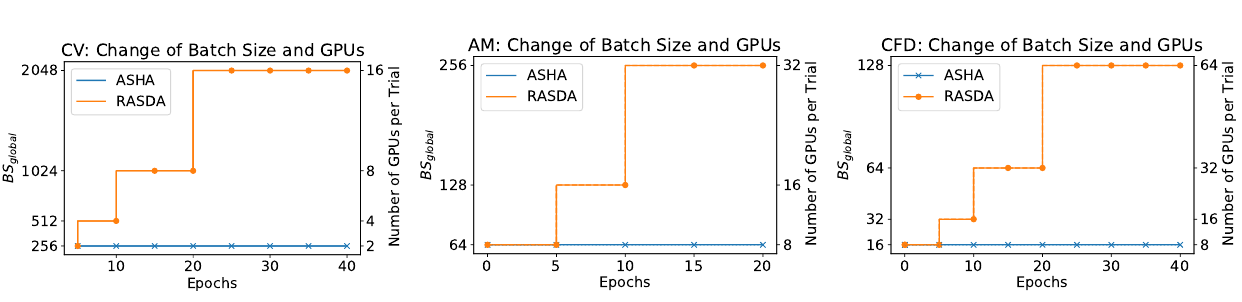
\includegraphics[width=\textwidth]{src/assets/trabalhos_relacionados/rasda_comparison.png}
\caption{Comparação entre o tamanho global do lote e o número de GPUs por \textit{trial} no ASHA e no RASDA, nos diferentes casos de aplicação}
\caption*{Fonte: \citefigure{Aach2025}}
\label{fig:rasda_comparison}
\end{figure}

\subsection{Comparative Analysis of TensorFlow and PyTorch for Image Classification using CNN with Parallelism Strategies}

\citeonline{Nandan10910577} investigou como o paralelismo de dados afeta o tempo de treinamento e a acurácia de CNNs de classificação de imagens em dois \textit{frameworks}, comparando a MirroredStrategy do TensorFlow com a DataParallel do PyTorch nos conjuntos CIFAR-10 e CIFAR-100. O modelo tem três camadas convolucionais seguidas por duas camadas densas. Cada \textit{framework} foi testado em modo sequencial e com paralelismo de dados, e foram coletados a acurácia de teste, o tempo de treinamento e as curvas de aprendizado.

No CIFAR-10, o paralelismo aumentou o tempo de treinamento, o que o autor atribui à sobrecarga de comunicação: o TensorFlow passou de 84,53 s para 144,6 s, e o PyTorch, de 210,42 s para 253,2 s. Com paralelismo, o PyTorch obteve acurácia maior (0,717, contra 0,680 do TensorFlow). As curvas das Figuras \ref{fig:tensorflow_results} e \ref{fig:pytorch_results} mostram, nos dois \textit{frameworks}, a acurácia de treino subindo ao longo das dez épocas enquanto a de validação se estabiliza perto de 0,70, com distância crescente entre as duas; as curvas do PyTorch com e sem paralelismo são quase iguais, e as do TensorFlow diferem mais entre si. No CIFAR-100, o paralelismo reduziu os tempos de treinamento: o do TensorFlow de 224,23 s para 202,84 s, e o do PyTorch de 373,45 s para 341,4 s. A acurácia do PyTorch subiu de 0,43 para 0,45, e a do TensorFlow caiu de 0,46 para 0,42.

O autor associa o TensorFlow à prototipagem rápida e o PyTorch a aplicações em que a acurácia é prioritária, mas os experimentos medem apenas tempo de treinamento e acurácia no CIFAR; nada neles avalia prototipagem ou uso em produção. Do mesmo modo, o paralelismo aumentou o tempo no CIFAR-10 e o reduziu no CIFAR-100, mas os dois conjuntos têm o mesmo número e o mesmo tamanho de imagens e diferem apenas no número de classes, de modo que esses resultados não bastam para atribuir a diferença à escala do problema. O que eles mostram, e que interessa a este trabalho, é que a sobrecarga de coordenar a execução paralela pode superar o ganho.

\begin{figure}[H]
    \centering
    \captionsetup{justification=centering}
    \caption{Curvas de acurácia de treino e de validação do TensorFlow com as estratégias sequencial e de paralelismo de dados no CIFAR-10}
    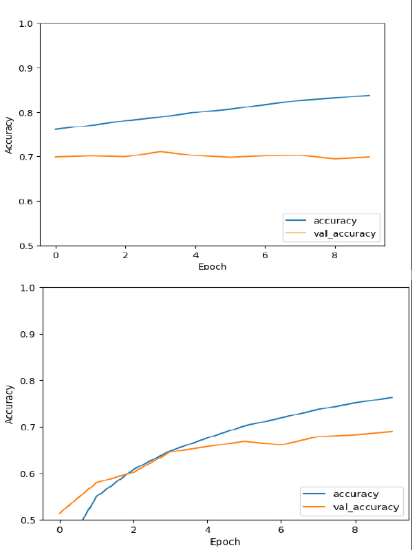
\includegraphics[width=0.33\textwidth]{src/assets/trabalhos_relacionados/comparative_analysis_of_tensorflow_and_pytorch_for_image_classification_using_cnn_with_parallelism_strategies_1.png}\\
    \captionsetup{justification=raggedright}
    \caption*{Fonte: \citefigure{Nandan10910577}}
    \label{fig:tensorflow_results}
\end{figure}

\begin{figure}[H]
    \centering
    \captionsetup{justification=centering}
    \caption{Curvas de acurácia de treino e de validação do PyTorch com as estratégias sequencial e de paralelismo de dados no CIFAR-10}
    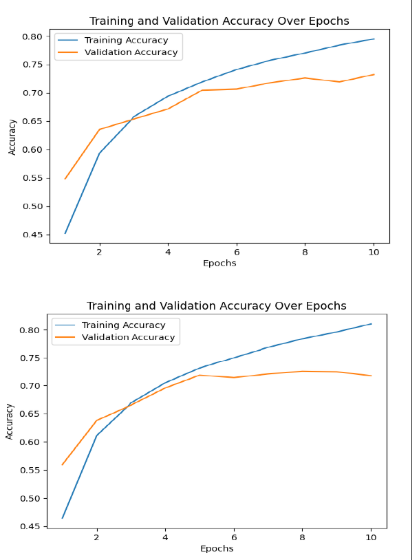
\includegraphics[width=0.33\textwidth]{src/assets/trabalhos_relacionados/comparative_analysis_of_tensorflow_and_pytorch_for_image_classification_using_cnn_with_parallelism_strategies_2.png}\\
    \captionsetup{justification=raggedright}
    \caption*{Fonte: \citefigure{Nandan10910577}}
    \label{fig:pytorch_results}
\end{figure}

\subsection{Avaliação de Fusão de Dados Espaciais com Espectrais para Classificação de Imagens Hiperespectrais}

O trabalho de \citeonline{Souza2023} é o ponto de partida deste estudo. O autor aborda a classificação de HSIs, em que há um compromisso entre complexidade computacional e acurácia, e observa que os métodos tradicionais se concentram nas características espectrais e subutilizam o contexto espacial, que pode melhorar a distinção entre classes. Os objetivos são avaliar o impacto do pré-processamento espacial na classificação por aprendizado de máquina, integrar a segmentação SEEDS a uma CNN 1D por concatenação, comparar o resultado com modelos de base e com o estado da arte, e quantificar o custo computacional da abordagem.

A metodologia propõe uma arquitetura híbrida que combina uma CNN 1D, para a classificação espectral, com o SEEDS, para a segmentação espacial. A Figura \ref{fig:metodologia_souza} mostra o fluxo completo, da separação dos conjuntos de dados à extração das métricas de avaliação. O processamento tem dois ramos independentes, executados em sequência: o ramo superior realiza PCA, definição de parâmetros, segmentação e concatenação das características espaciais; o ramo inferior executa PCA e vetorização, divisão dos dados de treino e classificação pela CNN 1D. Na implementação original, a CNN 1D tem quatro camadas convolucionais, com 16, 32, 64 e 64 filtros, seguidas por duas camadas densas, de 128 e 64 neurônios, e pela camada de saída (\autoref{tab:camadas}). A fusão é feita por uma camada de concatenação, que junta às características extraídas pelas convoluções o identificador do superpixel do pixel. Os hiperparâmetros da rede e do SEEDS foram ajustados manualmente: o autor relata ter alterado, por conjunto de dados, a paciência da parada antecipada e outros parâmetros de treino ao buscar o melhor resultado \cite{Souza2023}.

\begin{figure}[H]
    \centering
    \captionsetup{justification=centering}
    \caption{Fluxograma da metodologia proposta, com os ramos espacial e espectral, a fusão via concatenação, a classificação e a validação iterativa do modelo}
    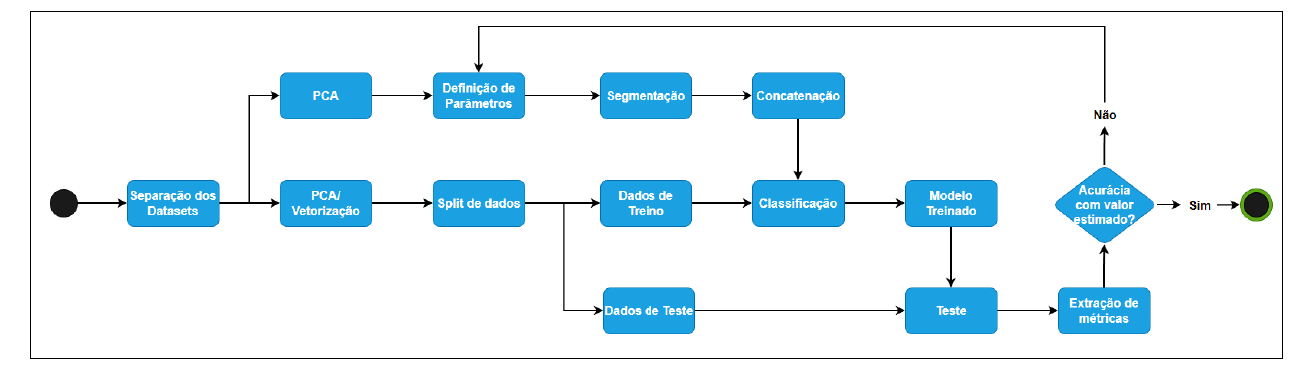
\includegraphics[width=\textwidth]{src/assets/trabalhos_relacionados/metodologia_souza.png}
    \captionsetup{justification=raggedright}
    \caption*{Fonte: \citefigure{Souza2023}}
    \label{fig:metodologia_souza}
\end{figure}

A validação experimental foi conduzida em três cenas: Indian Pines (21.025 pixels, 10.249 rotulados, 16 classes), Salinas Valley (111.104 pixels, 54.129 rotulados, 16 classes) e University of Pavia (207.400 pixels, 42.776 rotulados, 9 classes). As métricas avaliadas incluem Acurácia Geral (OA), Acurácia Média (AA), coeficiente Kappa, tempo de inferência e uso de memória. Com a fusão SEEDS, o autor reporta OA de 0,9142, AA de 0,8956 e Kappa de 0,9019 em Indian Pines, OA de 0,9928 em University of Pavia e OA de 0,9965 em Salinas Valley (\autoref{tab:linhaBase}); em Indian Pines, a fusão acrescentou 8,33, 8,79 e 9,47 pontos percentuais de OA, AA e Kappa à mesma rede sem a informação espacial. Essa configuração, com a fusão, é a referência contra a qual os ganhos deste trabalho são medidos. O fluxograma da Figura \ref{fig:metodologia_souza} mostra ainda o processo iterativo de treinamento, teste e extração de métricas, com validação baseada em um valor estimado de acurácia.

\subsection{Análise Comparativa dos Trabalhos Relacionados}

O \autoref{tab:trabRel} compara os três trabalhos com este. Os de \citeonline{Aach2025} e \citeonline{Nandan10910577} tratam de otimização, de hiperparâmetros em escala e de paralelismo no treinamento, respectivamente, mas em problemas de visão computacional, fluidodinâmica e manufatura aditiva, sem HSIs nem segmentação. O de \citeonline{Souza2023} trata de HSIs com fusão espectral-espacial, mas executa as etapas em sequência, ajusta os hiperparâmetros à mão e usa um único segmentador. Nenhum dos três combina, no mesmo fluxo de classificação de HSIs, a busca automática de hiperparâmetros da rede e do segmentador, a comparação de segmentadores sob a mesma otimização e o paralelismo entre as etapas; é essa a lacuna que este trabalho ocupa.

\begin{quadro}[H]
    \centering
    \caption{Comparação dos trabalhos relacionados}
    \resizebox{\textwidth}{!}{%
    \begin{tabular}{|p{0.20\textwidth}|p{0.19\textwidth}|p{0.19\textwidth}|p{0.19\textwidth}|p{0.19\textwidth}|}
        \hline
        \rowcolor[HTML]{EFEFEF}
        \textbf{Característica} & \textbf{\cite{Aach2025}} & \textbf{\cite{Nandan10910577}} & \textbf{\cite{Souza2023}} & \textbf{Este Trabalho} \\
        \hline
        \textbf{Arquitetura de IA} & 
        ResNet50 (ImageNet), autoencoder convolucional (CFD) e SwinTransformer (AM) &
        CNN customizada&
        CNN 1D& 
        CNN 1D otimizada com fusão espectral-espacial \\
        \hline
        \textbf{Processamento Paralelo} & 
        Sim. RASDA&
        Sim. Paralelismo de dados (MirroredStrategy e DataParallel) &
        Não. Ramos independentes, executados em sequência &
        Sim. Threads e processos: entre os ramos do pré-processamento, por partição da cena e na fusão concorrente\\
        \hline
        \textbf{Segmentação} & 
        Não aplicado & 
        Não aplicado & 
        Sim. SEEDS ajustado manualmente & 
        Sim. SEEDS, SLIC, LSC e Watershed sob otimização conjunta \\
        \hline
        \textbf{HPO} & 
        Sim. ASHA e RASDA &
        Não abordada &
        Não. Ajuste manual por conjunto de dados &
        Sim. Busca aleatória, TPE e algoritmo genético para CNN e segmentação \\
        \hline
        \textbf{Métricas} & 
        Val MSE, Test MSE, Runtime, Relative Error & 
        Test Accuracy, Training Time, Val Accuracy & 
        OA, AA, Kappa, Tempo, Memória & 
        OA, AA, Kappa, Tempo, Memória, \textit{Speedup} \\
        \hline
        \textbf{Datasets} & 
        ImageNet, CFD, RAISE-LPBF& 
        CIFAR-10, CIFAR-100& 
        Indian Pines, Salinas, Pavia& 
        Indian Pines, Salinas Valley, University of Pavia \\
        \hline
        \textbf{Tecnologias} & 
        Python, PyTorch, Horovod, DeepSpeed, Ray Tune, CUDA 11.5, NVIDIA DALI& 
        Python, TensorFlow, PyTorch, Keras, CUDA& 
        Python, TensorFlow, Keras, scikit-learn, OpenCV, Google Colab&
        Python, PyTorch, scikit-learn, OpenCV, Optuna\\
        \hline
    \end{tabular}%
    }
    \captionsetup{justification=raggedright}
    \caption*{Fonte: Elaborado pelo autor}
    \label{tab:trabRel}
\end{quadro} \clearpage
\chapter{Projeto}
\label{cap:proj}

Neste trabalho será proposta a implementação de estratégias de otimização de classificação de imagens hiperespectrais utilizando CNNs 1D combinadas com técnicas de segmentação espacial. A partir de arquiteturas e algoritmos encontrados na literatura, procura-se fazer uma análise com base nas métricas elencadas neste projeto. O capítulo está organizado da seguinte forma: inicialmente é apresentada a visão geral do sistema proposto. Na sequência, são dispostas as premissas que norteiam o desenvolvimento. Posteriormente, são descritos os materiais e métodos utilizados e os requisitos levantados, seguidos do detalhamento da arquitetura do sistema e dos algoritmos. Ao fim, são apresentados o plano de verificação, a análise de riscos e o cronograma de atividades.

\section{Visão Geral}

O projeto visa paralelizar o processamento da arquitetura de \citeonline{Souza2023} e automatizar o ajuste de hiperparâmetros tanto do modelo de classificação quanto dos algoritmos de segmentação. As técnicas específicas são detalhadas na \autoref{subsec:algoritmos}.

Para a avaliação da eficácia e do custo computacional das otimizações propostas, serão utilizados três datasets de referência na área: Indian Pines, Salinas Valley e University of Pavia. Os detalhes da campanha de experimentos são abordados na \autoref{subsec:campanhaExperimental}.

A \autoref{fig:visaoGeral} sumariza a relação entre os principais componentes do sistema proposto. A arquitetura híbrida processa simultaneamente as características espectrais via CNN 1D e as características espaciais via algoritmos de segmentação, realizando a fusão dos dados através de uma camada de concatenação. O processo de otimização de hiperparâmetros é controlado por algoritmos automatizados que ajustam tanto os parâmetros da rede neural quanto os parâmetros de segmentação.

\begin{figure}[H]
    \centering
    \captionsetup{justification=centering}
    \caption{Principais componentes do projeto}
     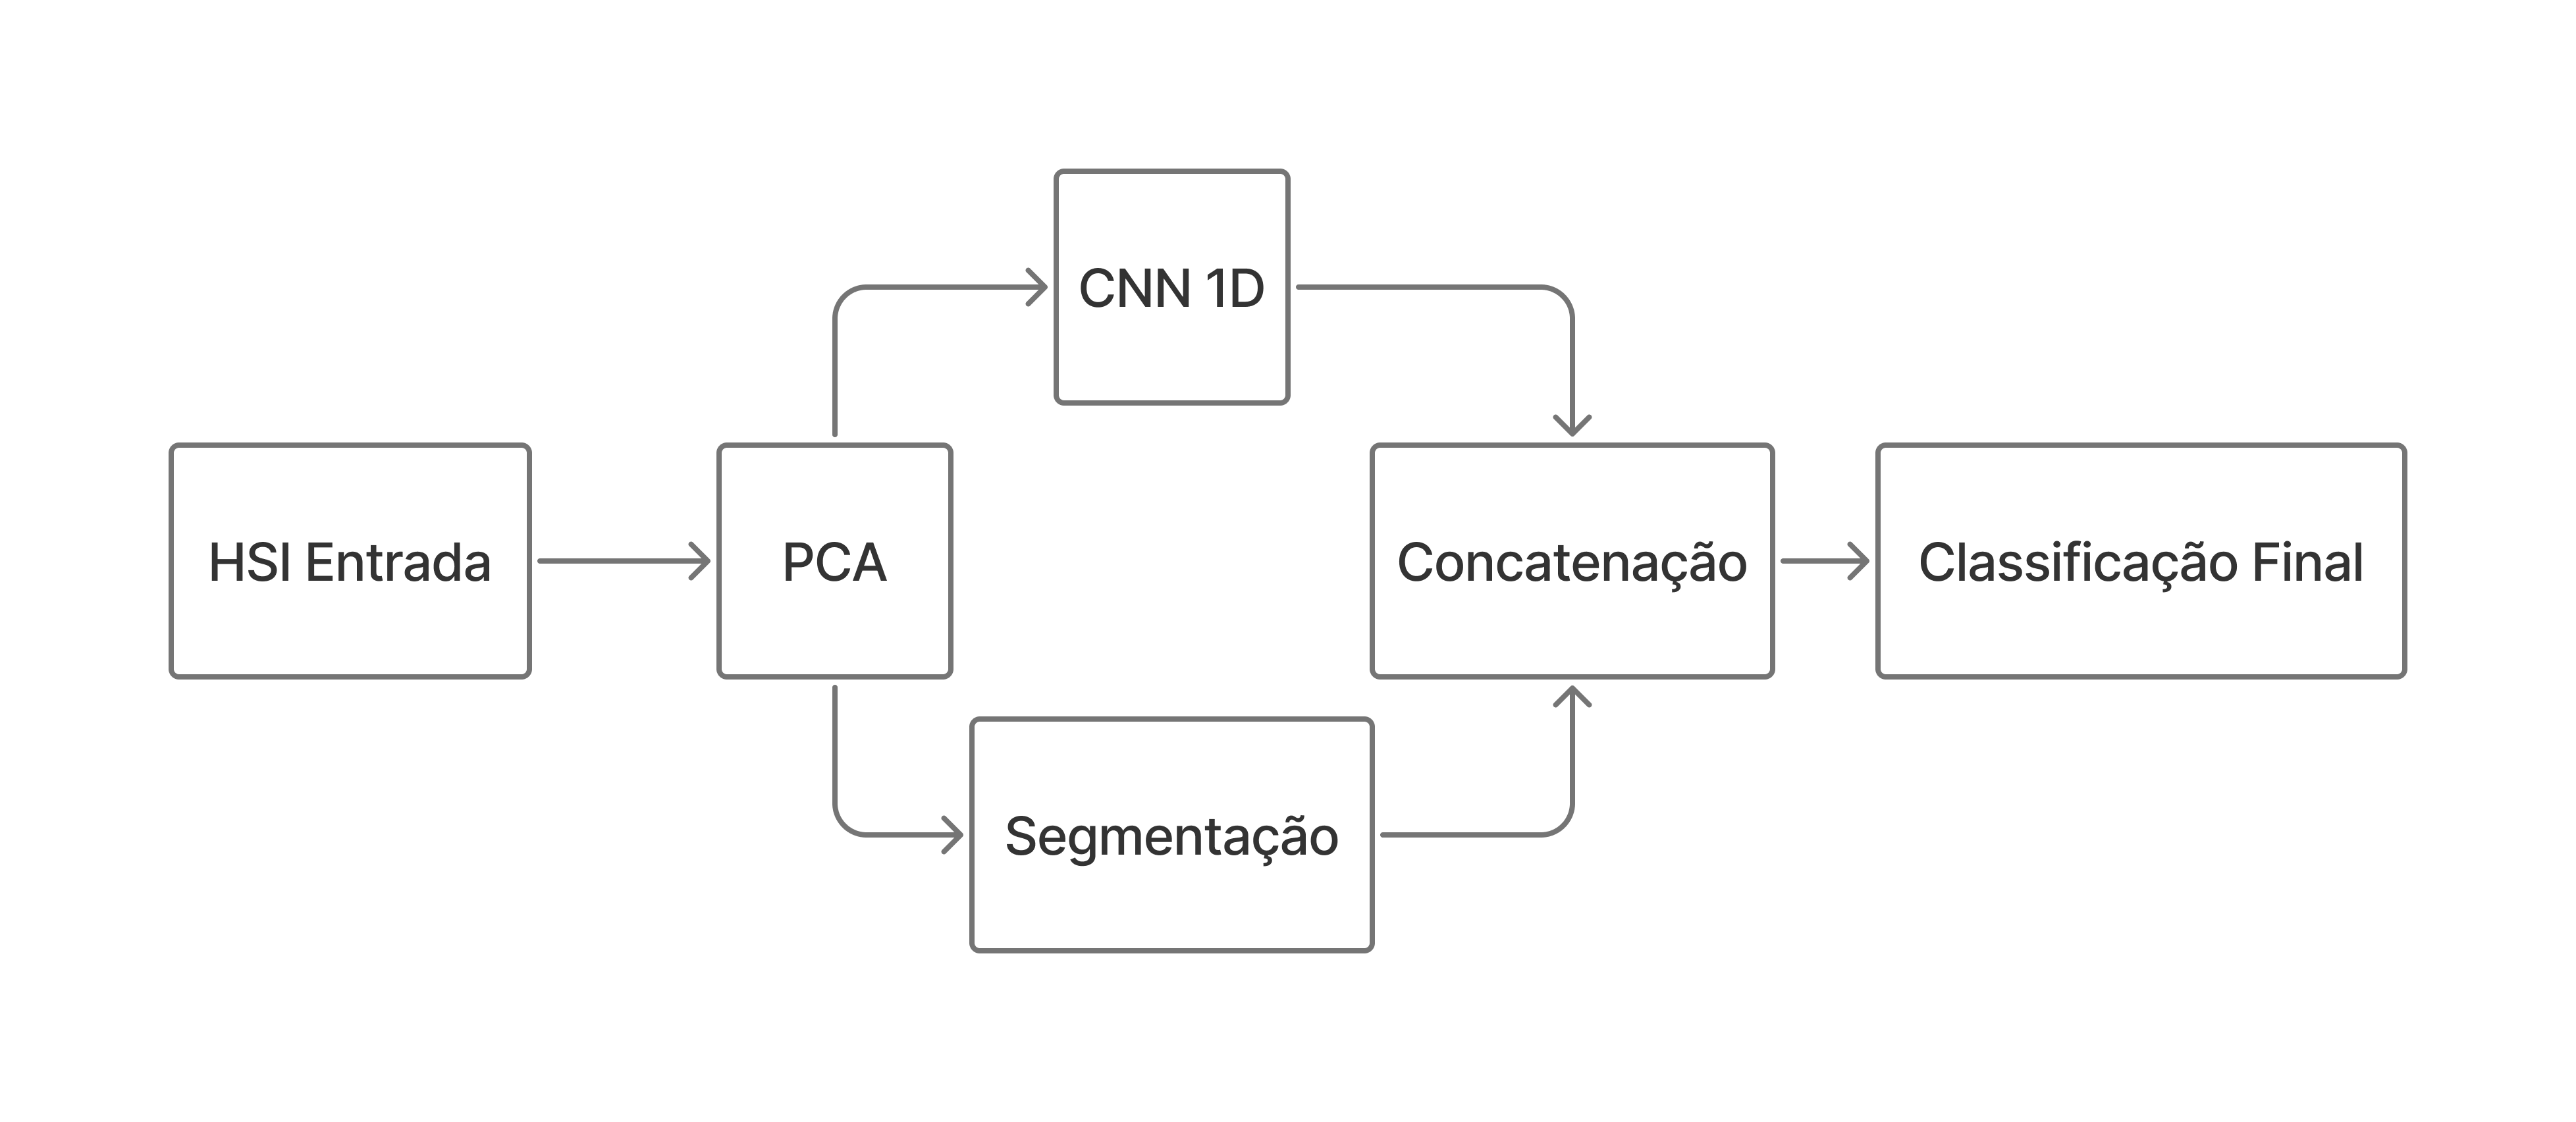
\includegraphics[width=0.8\textwidth]{src/assets/projeto/visaoGeral.png}\\
    \captionsetup{justification=raggedright}
    \caption*{Fonte: Elaborada pelo autor}
    \label{fig:visaoGeral}
\end{figure}

\section{Premissas}

O trabalho parte do pressuposto de que a arquitetura base proposta por \citeonline{Souza2023}, que combina CNN 1D com segmentação SEEDS, apresenta gargalos de processamento que podem ser mitigados por técnicas de paralelização e otimização automática de hiperparâmetros. Especificamente, assume-se que o processamento sequencial das etapas de segmentação e classificação pode ser acelerado executando-as de forma concorrente; a fração do tempo de execução ocupada por cada etapa será medida na campanha experimental.

Será considerado que os três datasets selecionados (Indian Pines, com 16 classes e 10.249 pixels rotulados de um total de 21.025; Salinas Valley, com 16 classes e 54.129 rotulados de 111.104; e University of Pavia, com 9 classes e 42.776 rotulados de 207.400) são representativos o suficiente para validar as melhorias propostas e permitir a comparação direta com \citeonline{Souza2023}, que utilizou as mesmas cenas.

Presume-se que a separação de 85\% das amostras para treinamento e 15\% para validação e teste, divididos igualmente entre os dois, conforme adotado por \citeonline{Souza2023} e \citeonline{Viel10064297}, é adequada para avaliar o desempenho dos modelos.

Quanto à otimização de hiperparâmetros, será assumido que técnicas de busca automatizada como Grid Search e Otimização Bayesiana são capazes de encontrar configurações próximas ao ótimo global dentro de um espaço de busca adequadamente definido.

Em relação ao processamento paralelo, presume-se que a paralelização das etapas de segmentação e classificação espectral pode reduzir significativamente o tempo total de processamento, dado que essas operações apresentam independência de dados durante parte do fluxo de execução.

Sob essas premissas, os experimentos controlados medirão os ganhos relativos de cada otimização proposta sobre a configuração de \citeonline{Souza2023}.

\section{Metodologia}

\subsection{Materiais}

\subsubsection{Ambiente Computacional e Ferramentas}

O desenvolvimento e experimentação serão realizados utilizando a linguagem Python com as seguintes bibliotecas principais: TensorFlow/Keras ou PyTorch para implementação da CNN 1D, Scikit-Learn para pré-processamento (PCA) e métricas, OpenCV para manipulação de imagens, e Ray Tune para otimização de hiperparâmetros.

Os experimentos computacionalmente intensivos serão executados em ambiente de computação de alto desempenho (HPC) ou Google Colab Pro com acesso a GPUs. Para experimentos preliminares e desenvolvimento, será utilizado ambiente local com CPU de múltiplos núcleos.

\subsubsection{Datasets Hiperespectrais}

Serão utilizados três datasets públicos de imagens hiperespectrais, os mesmos avaliados por \citeonline{Souza2023} (\autoref{tab:trabRel}), ilustrados nas Figuras \ref{fig:indian_pines}, \ref{fig:salinas_valley} e \ref{fig:pavia_university}.

O dataset Indian Pines (\autoref{fig:indian_pines}) representa uma área agrícola capturada em 1992 pelo sensor AVIRIS no noroeste de Indiana. A imagem possui 145×145 pixels, com resolução espacial de 20 metros por pixel; dos seus 21.025 pixels, 10.249 são rotulados em 16 classes de cobertura do solo. Das 224 bandas originais capturadas pelo sensor, foram utilizadas 200 bandas espectrais na faixa de 400 a 2500 nanômetros com intervalos de 10 nanômetros, após a remoção de 4 bandas nulas e 20 bandas comprometidas pela absorção atmosférica de água. A visualização apresenta a composição em falsa-cor à esquerda, o mapa de verdade terrestre ao centro e a legenda com as 16 classes, que incluem diferentes tipos de culturas agrícolas (alfafa, milho, soja, trigo), pastagens, matas e áreas construídas \cite{LabanReduced3D}.

\begin{figure}[H]
    \centering
    \captionsetup{justification=centering}
    \caption{Indian Pines: composição falsa-cor, mapa de verdade terrestre e legenda}
    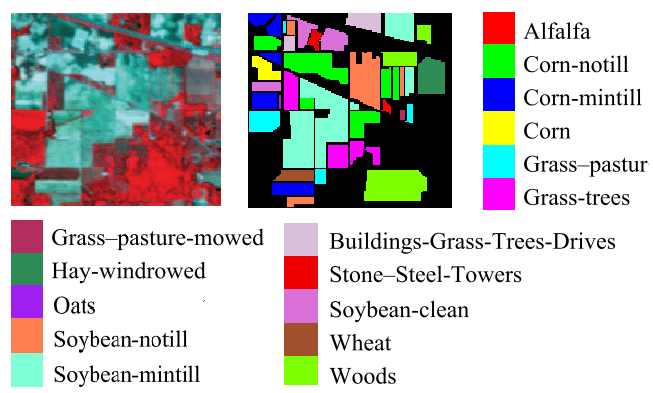
\includegraphics[width=0.8\textwidth]{src/assets/projeto/indian-pines_dataset_visualization.png}\\
    \captionsetup{justification=raggedright}
    \caption*{Fonte: \citefigure{LabanReduced3D}}
    \label{fig:indian_pines}
\end{figure}

O dataset Salinas Valley (\autoref{fig:salinas_valley}) foi capturado pelo sensor AVIRIS na região do Vale de Salinas, Califórnia, com resolução espacial de 3,7 metros por pixel. A imagem possui 512×217 pixels e originalmente continha 224 bandas espectrais; após a remoção de 20 bandas afetadas pela absorção de água, restaram 204 bandas utilizáveis para análise. Dos 111.104 pixels da imagem, 54.129 são rotulados em 16 classes, predominantemente culturas agrícolas e tipos de cobertura do solo. A imagem (a) mostra a composição falsa-cor da área agrícola, (b) apresenta o mapa de verdade terrestre e (c) exibe a legenda com as 16 classes, que incluem duas classes de brócolis, alface romana em diferentes estágios, vinhedos, solo em pousio e outras culturas \cite{Li2022Directionally}.

\begin{figure}[H]
    \centering
    \captionsetup{justification=centering}
    \caption{Salinas Valley: (a) falsa-cor, (b) verdade terrestre, (c) legenda}
    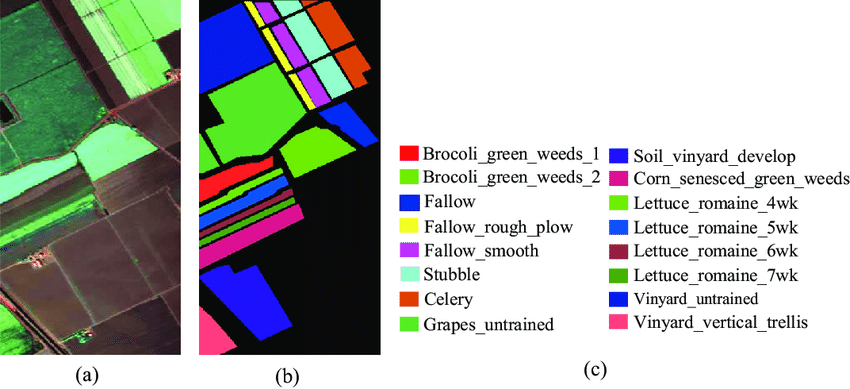
\includegraphics[width=0.85\textwidth]{src/assets/projeto/salinas_valley_dataset_visualization.png}\\
    \captionsetup{justification=raggedright}
    \caption*{Fonte: \citefigure{Li2022Directionally}}
    \label{fig:salinas_valley}
\end{figure}

Por fim, o dataset University of Pavia (\autoref{fig:pavia_university}) representa uma área urbana da Universidade de Pavia, Itália, capturada em 2003 pelo sensor ROSIS. A imagem possui 610×340 pixels, com resolução espacial de 1,3 metro por pixel. Das 115 bandas espectrais originais, capturadas na faixa de comprimento de onda entre 0,43 e 0,86 micrômetro (430 a 860 nanômetros), foram utilizadas 103 bandas, após a remoção de 12 bandas contaminadas por ruído. Dos 207.400 pixels da imagem, 42.776 são rotulados em 9 classes de cobertura urbana. A visualização mostra em (a) a composição falsa-cor da área universitária, em (b) o mapa de verdade terrestre das estruturas urbanas e a legenda com as 9 classes que incluem asfalto, prados, cascalho, árvores, chapas metálicas pintadas, solo exposto, betume, tijolos autoblocantes e sombras \cite{Qi2019Spectral}.

\begin{figure}[H]
    \centering
    \captionsetup{justification=centering}
    \caption{University of Pavia: (a) falsa-cor, (b) verdade terrestre e legenda}
    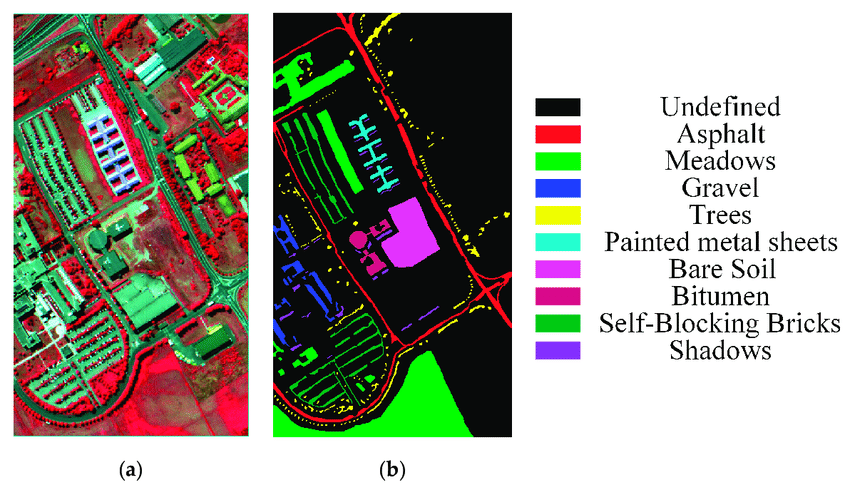
\includegraphics[width=0.7\textwidth]{src/assets/projeto/university_of_pavia_dataset_visualization.png}\\
    \captionsetup{justification=raggedright}
    \caption*{Fonte: \citefigure{Qi2019Spectral}}
    \label{fig:pavia_university}
\end{figure}

Para versionamento de código será utilizado Git, e para documentação e reprodutibilidade dos experimentos será mantido registro detalhado de todas as configurações utilizadas através de arquivos de configuração e notebooks Jupyter.

\subsection{Métodos}

Serão utilizadas as seguintes técnicas e estratégias de otimização: paralelização do processamento espacial e espectral, otimização automática de hiperparâmetros (Grid Search e Otimização Bayesiana), comparação de diferentes algoritmos de segmentação como SEEDS, LSC e Watershed, e redução dimensional via PCA. Cada técnica é detalhada na \autoref{subsec:algoritmos}.

A coleta de métricas será realizada utilizando as ferramentas nativas do TensorFlow/Keras ou do PyTorch para monitoramento do treinamento, bibliotecas de \textit{profiling} do Python para medição do tempo de execução e utilitários do sistema para medição do uso de memória. As métricas principais são a Acurácia Geral (OA) e a Acurácia Média (AA) \cite{Congalton1991}, o coeficiente Kappa \cite{Cohen1960}, os tempos de treinamento e de inferência, o uso de memória e o \textit{speedup} obtido com a paralelização.

A fim de promover a reutilização de código e facilitar a reprodução dos experimentos, será implementado um \textit{framework} modular que abstrai os componentes principais do sistema: módulo de pré-processamento, módulo de segmentação, módulo de classificação CNN, módulo de fusão e módulo de avaliação. A interação entre esses módulos é detalhada na \autoref{subsec:arquitetura}.

\section{Análise de Requisitos}
\label{sec:req}

\begin{quadro}[H]
    \centering
    \caption{Requisitos funcionais}
    \begin{tabular}{|p{0.125\textwidth}|p{0.8\textwidth}|}
        \hline
        \rowcolor[HTML]{C0C0C0}
        \textbf{Requisito} & \textbf{Descrição}  \\
        \hline
        
        \textbf{RF01} & A arquitetura deve classificar HSIs utilizando CNN 1D para extração de características espectrais \\ 
        \hline

        \textbf{RF02} & A arquitetura deve implementar algoritmos de segmentação espacial \\
        \hline

        \textbf{RF03} & A arquitetura deve realizar fusão de dados espectrais e espaciais \\
        \hline
        
        \textbf{RF04} & O sistema deve implementar otimização automática de hiperparâmetros \\
        \hline

        \textbf{RF05} & O sistema deve produzir métricas de desempenho e custo computacional \\
        \hline
        
        \textbf{RF06} & O sistema deve implementar paralelização do processamento espacial e espectral \\
        \hline
    \end{tabular}
    \label{tab:rf}
\end{quadro}

\begin{quadro}[H]
    \centering
    \caption{Requisitos não funcionais}
    \begin{tabular}{|p{0.125\textwidth}|p{0.8\textwidth}|}
       \hline
        \rowcolor[HTML]{C0C0C0}
        \textbf{Requisito} & \textbf{Descrição}  \\
        \hline
        
        \textbf{RNF01} & O classificador espectral deve ser uma CNN 1D baseada no modelo de \citeonline{Souza2023} e \citeonline{Viel10064297} \\
        \hline
        
        \textbf{RNF02} & Toda a arquitetura deve ser desenvolvida na linguagem de programação Python \\
        \hline

        \textbf{RNF03} & Para treinar, testar e validar o modelo deve ser utilizada a plataforma Google Colab ou ambiente HPC com GPU \\
        \hline

        \textbf{RNF04} & A fusão de dados deve ser realizada por concatenação dos segmentos espaciais com as características espectrais na CNN \\
        \hline

        \textbf{RNF05} & A otimização automática de hiperparâmetros deve melhorar as métricas de acurácia (OA, AA, Kappa) em comparação ao ajuste manual \\
        \hline

        \textbf{RNF06} & O sistema deve produzir resultados reprodutíveis através de registro detalhado de configurações \\
        \hline
        
        \textbf{RNF07} & A paralelização deve alcançar redução mensurável no tempo de processamento em relação à implementação sequencial \\
        \hline
    \end{tabular}
    \label{tab:rnf}
\end{quadro}

\subsection{Arquitetura do Sistema} 
\label{subsec:arquitetura}

A arquitetura proposta segue uma organização modular que permite experimentação com diferentes configurações. A \autoref{fig:arquiteturaSistema} apresenta o diagrama de blocos detalhado do sistema completo.

\begin{figure}[H]
    \centering
    \captionsetup{justification=centering}
    \caption{Arquitetura modular do sistema}
     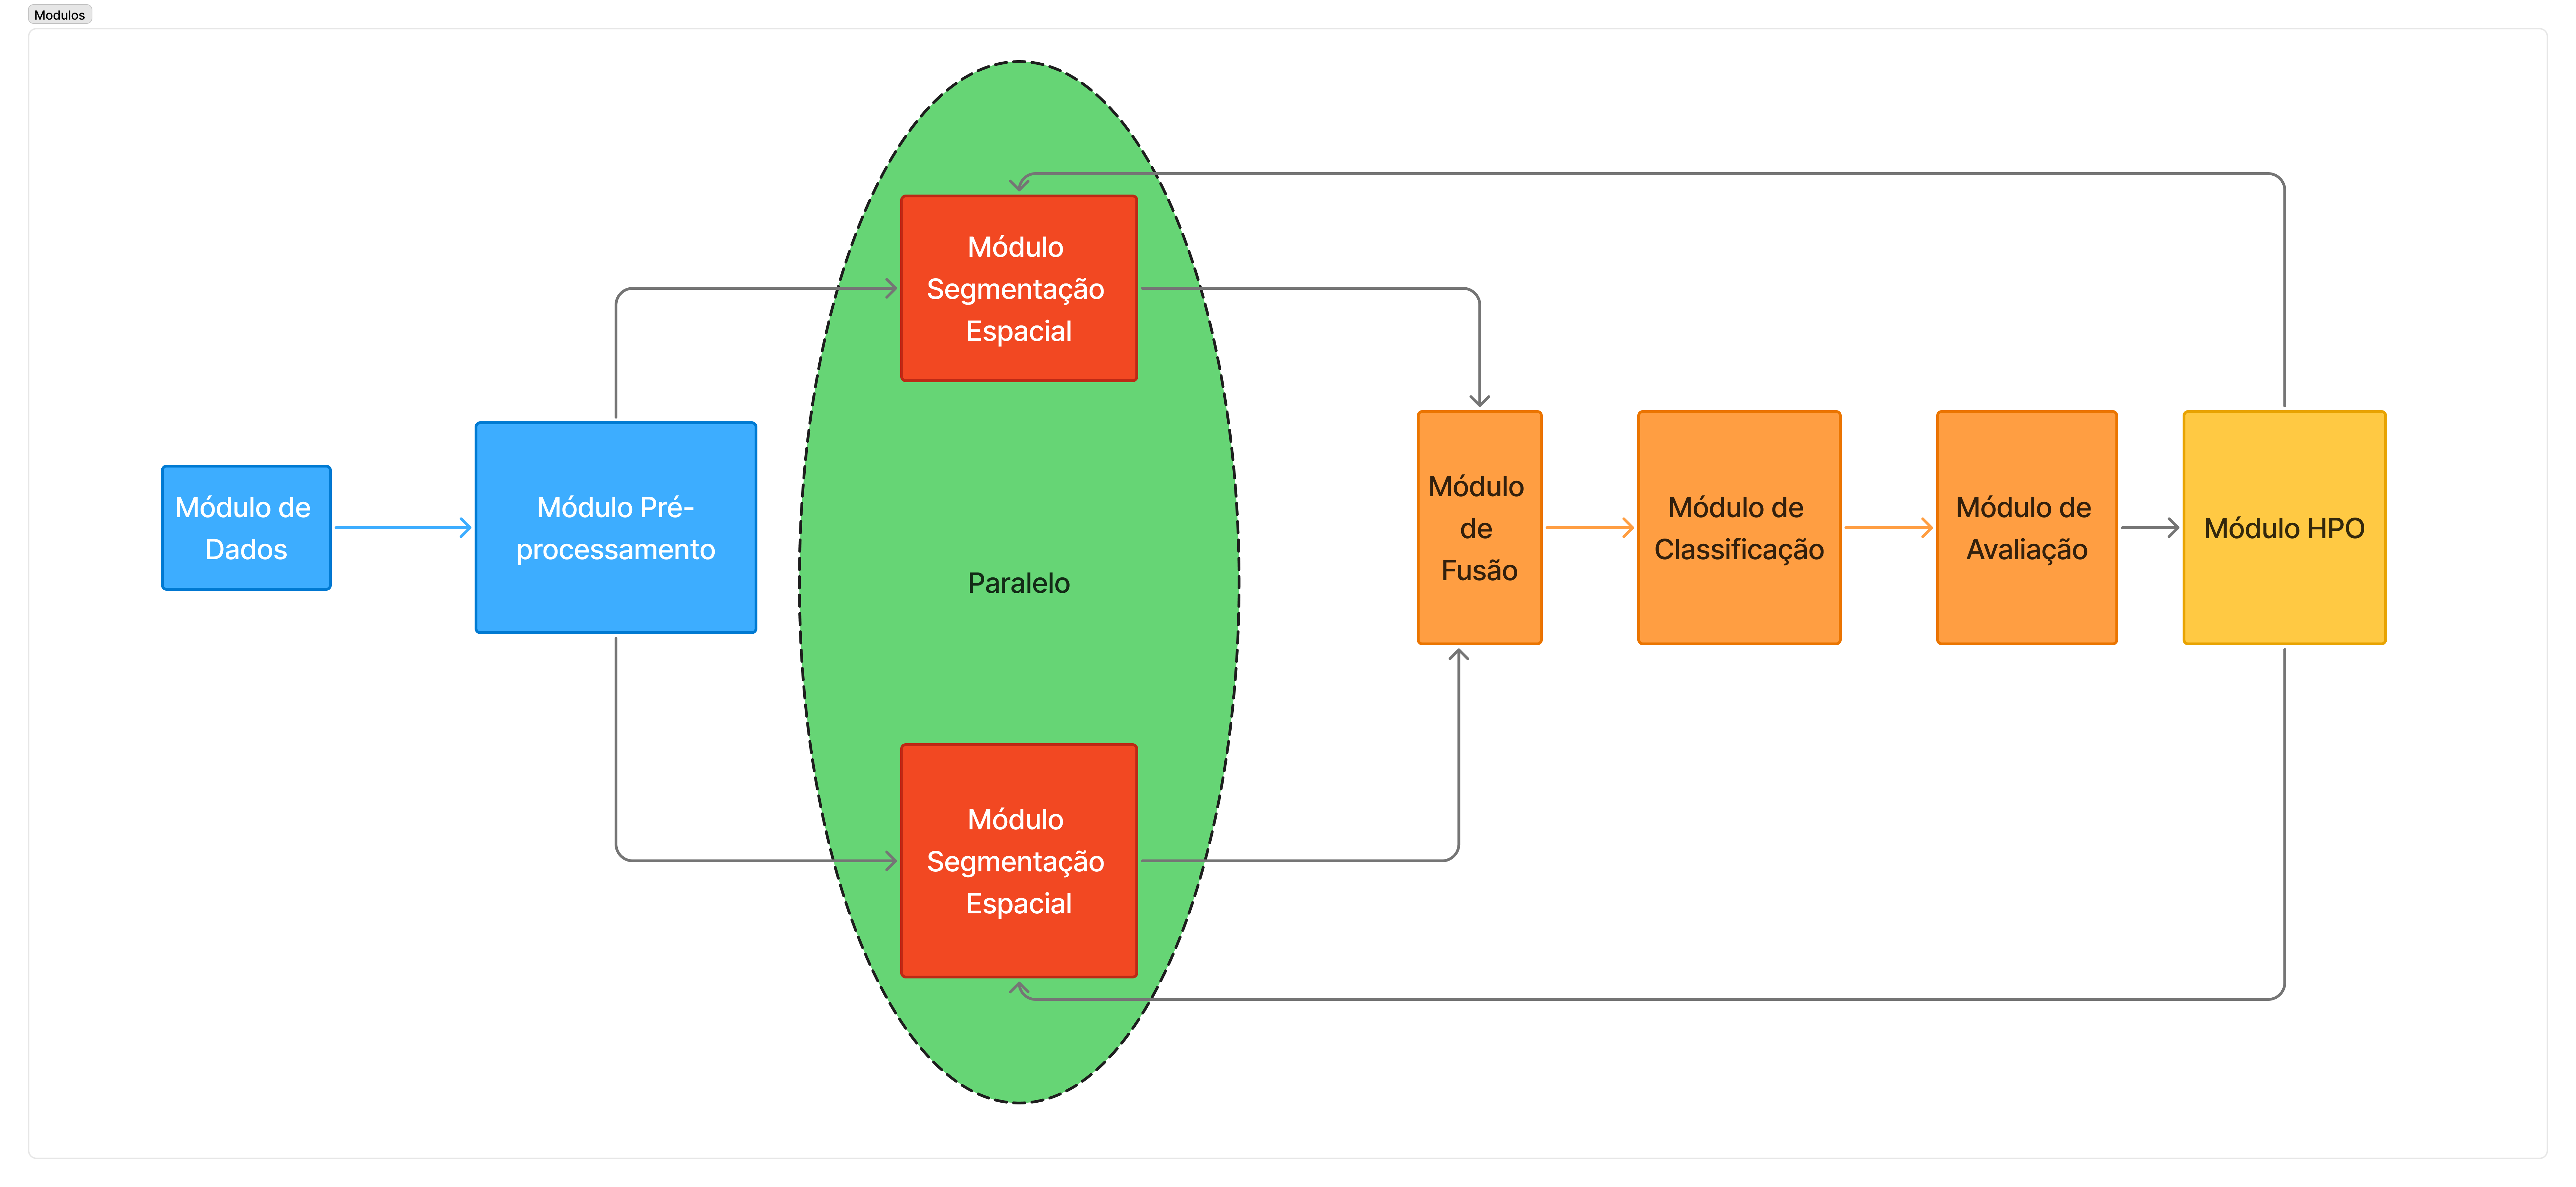
\includegraphics[width=0.9\textwidth]{src/assets/projeto/arquiteturaSistema.png}\\
    \captionsetup{justification=raggedright}
    \caption*{Fonte: Elaborada pelo autor}
    \label{fig:arquiteturaSistema}
\end{figure}

A arquitetura proposta organiza-se em módulos funcionais que operam de forma integrada. O Módulo de Dados é responsável pelo carregamento e preparação dos datasets, abstraindo as diferenças entre formatos distintos e fornecendo uma interface unificada para o sistema, além de realizar a separação dos conjuntos de treino, validação e teste com base em \citeonline{Souza2023} e \citeonline{Viel10064297}.

O processamento dos dados ocorre em duas frentes paralelas. De um lado, o Módulo de Pré-processamento aplica a técnica de PCA para redução dimensional, transformando o hipercubo espectral original em um conjunto reduzido de componentes principais cujo número pode ser configurado conforme necessário. Do outro, o Módulo de Segmentação Espacial implementa os algoritmos SEEDS, LSC e Watershed de forma intercambiável, produzindo mapas de superpixels que capturam a estrutura espacial das imagens.

As características espectrais resultantes do pré-processamento são então alimentadas ao Módulo CNN 1D, que implementa uma rede neural convolucional unidimensional com arquitetura configurável, composta por camadas de convolução 1D seguidas de camadas densas totalmente conectadas. Este módulo extrai características discriminativas de cada pixel a partir de sua assinatura espectral.

O Módulo de Fusão realiza a concatenação entre as características espectrais extraídas pela CNN 1D e os rótulos de superpixels provenientes da segmentação espacial, unindo as informações complementares em um único vetor de características. Essas características fusionadas são então processadas pelo Módulo de Classificação, que realiza a predição final das classes para cada pixel da imagem.

O Módulo de Avaliação quantifica o desempenho do sistema através de métricas de acurácia e custo computacional. Por fim, o Módulo de Otimização de Hiperparâmetros coordena a busca automática dos melhores parâmetros tanto para os algoritmos de segmentação quanto para a arquitetura da CNN, utilizando técnicas como Grid Search ou Otimização Bayesiana para maximizar o desempenho global do sistema.

\subsection{Algoritmos e Técnicas} 
\label{subsec:algoritmos}

A otimização e a classificação de imagens hiperespectrais combinarão técnicas de aprendizado profundo, processamento de imagens e otimização automática, descritas a seguir.

\subsubsection{Redução Dimensional via PCA}

A técnica de Análise de Componentes Principais (PCA) será aplicada para reduzir a dimensionalidade espectral das imagens hiperespectrais. Dado um conjunto de dados com $n$ bandas espectrais, o PCA identifica as $k$ componentes principais (onde $k < n$) que capturam a maior variância dos dados \cite{Jolliffe2002}.

\subsubsection{Rede Neural Convolucional 1D (CNN 1D)}

A arquitetura da CNN 1D é projetada para processar as características espectrais unidimensionais de cada pixel. A arquitetura base consiste em:

\begin{itemize}
    \item 4 camadas convolucionais 1D com 16, 32, 64 e 128 filtros respectivamente
    \item Função de ativação ReLU após cada camada convolucional
    \item Operações de \textit{max-pooling} para redução dimensional
    \item 3 camadas densas (totalmente conectadas) com \textit{dropout} para regularização \cite{Dropout:asimplewaytopreventneuralnetworksfromoverfitting}
    \item Camada de saída com ativação \textit{softmax} para classificação multiclasse
\end{itemize}

\begin{figure}[H]
    \centering
    \captionsetup{justification=centering}
    \caption{Arquitetura detalhada da CNN 1D}
    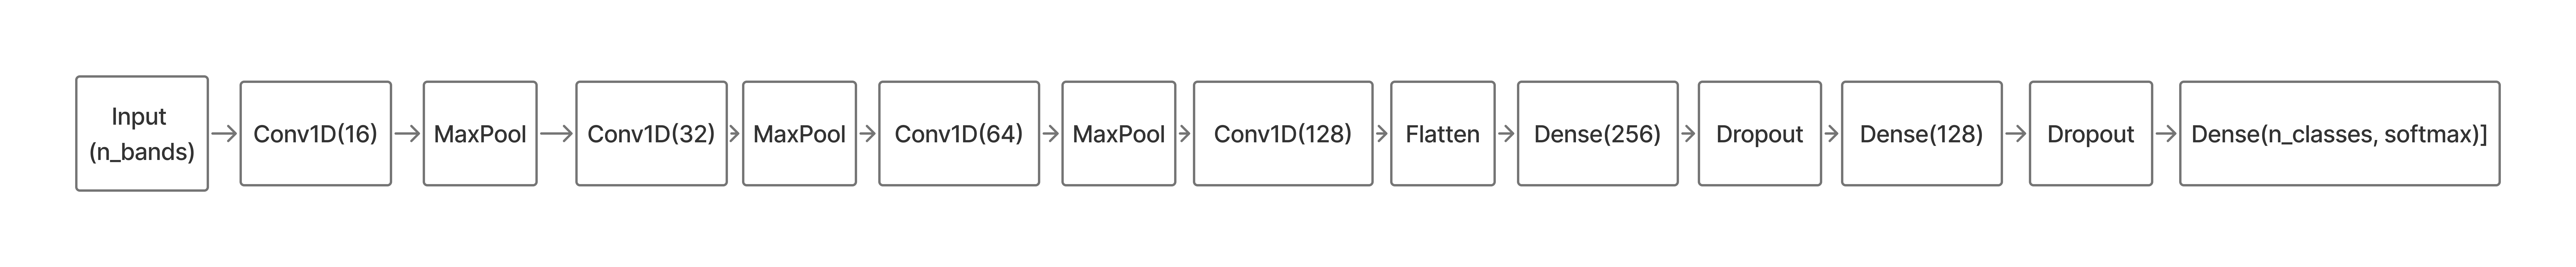
\includegraphics[width=0.9\textwidth]{src/assets/projeto/arquiteturaCNN.png}\\
    \captionsetup{justification=raggedright}
    \caption*{Fonte: Elaborada pelo autor}
    \label{fig:arquiteturaCNN}
\end{figure}

Os hiperparâmetros da rede (número de filtros, tamanho dos \textit{kernels}, taxa de \textit{dropout}, taxa de aprendizado, otimizador) serão otimizados automaticamente pelo módulo de HPO.

\subsubsection{Algoritmos de Segmentação Espacial}

Três algoritmos de segmentação serão implementados e comparados:

\begin{itemize}
    \item \textbf{SEEDS} (\textit{Superpixels Extracted via Energy-Driven Sampling}): parte de uma grade regular de superpixels e refina as fronteiras por \textit{hill-climbing}, transferindo blocos de pixels e, depois, pixels individuais entre superpixels vizinhos sempre que a troca aumenta uma função de energia que favorece a homogeneidade de cor de cada superpixel e fronteiras regulares. Os principais parâmetros ajustáveis são o número desejado de superpixels, o número de iterações e o número de níveis de blocos usados no refinamento \cite{bergh2013seedssuperpixelsextractedenergydriven}.
    \item \textbf{LSC} (\textit{Linear Spectral Clustering}): realiza agrupamento espectral considerando tanto a cor quanto a posição espacial dos pixels. Os principais parâmetros são o número de superpixels, o peso da regularização espacial e o número de iterações \cite{Zhengqin7298741}.
    \item \textbf{Watershed}: algoritmo clássico de segmentação baseado em morfologia matemática, que trata a imagem como uma superfície topográfica. Os parâmetros são o método de marcação das sementes e o nível de compactação \cite{Najman546254}.
\end{itemize}

Cada algoritmo será executado sobre as três primeiras componentes principais obtidas via PCA, gerando um mapa de superpixels que identifica regiões espacialmente coerentes na imagem.

\subsubsection{Fusão de Características por Concatenação}

A fusão das características espectrais (extraídas pela CNN 1D) com as características espaciais (rótulos de superpixels) é realizada por uma camada de concatenação, como em \citeonline{Souza2023}, que concatena o identificador do superpixel como um único valor numérico. Neste projeto, está prevista a codificação do identificador em um vetor \textit{one-hot}. Para cada pixel:

\begin{enumerate}
    \item A CNN 1D extrai um vetor de características espectrais $\mathbf{f}_{\text{esp}} \in \mathbb{R}^{d}$;
    \item O algoritmo de segmentação atribui um rótulo de superpixel $l \in \{1, 2, \ldots, S\}$, em que $S$ é o número de superpixels;
    \item O rótulo é codificado como vetor \textit{one-hot} $\mathbf{f}_{\text{sp}} \in \mathbb{R}^{S}$;
    \item As características são concatenadas: $\mathbf{f} = [\mathbf{f}_{\text{esp}}, \mathbf{f}_{\text{sp}}]$.
\end{enumerate}

\begin{figure}[H]
    \centering
    \captionsetup{justification=centering}
    \caption{Processo de fusão por concatenação}
    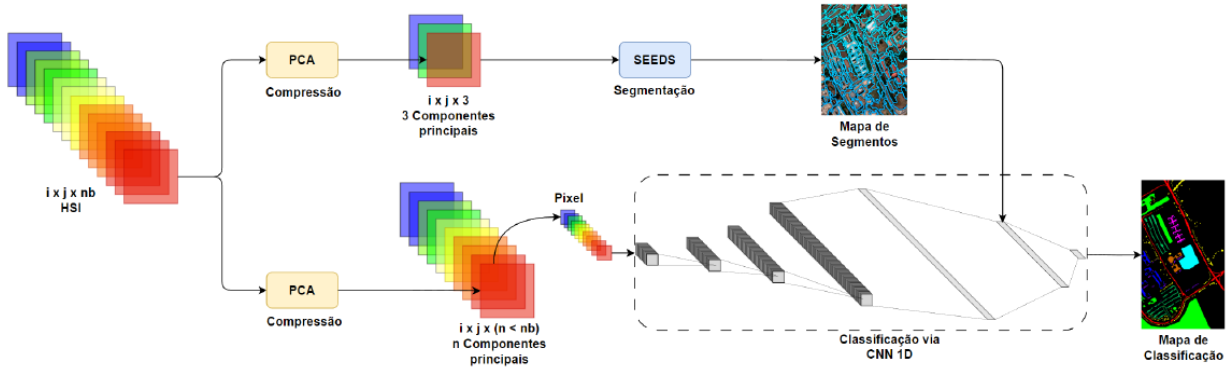
\includegraphics[width=0.9\textwidth]{src/assets/projeto/fusaoConcatenacao.png}\\
    \captionsetup{justification=raggedright}
    \caption*{Fonte: \citefigure{Souza2023}}
    \label{fig:fusaoConcatenacao}
\end{figure}

O vetor de características fusionadas é então alimentado a camadas densas adicionais que realizam a classificação final.

\subsubsection{Paralelização do Processamento}

Para acelerar o fluxo de processamento, a seguinte estratégia de paralelização será implementada, explorando a independência de dados entre as etapas de segmentação e classificação:

\textbf{Paralelização Inter-Etapas}: A segmentação espacial e a extração de características espectrais pela CNN são processos independentes que podem ser executados simultaneamente. Esta independência existe porque:
\begin{itemize}
    \item A segmentação opera sobre as componentes principais do PCA para gerar o mapa de superpixels, sem necessitar das características extraídas pela CNN.
    \item A CNN 1D processa os vetores espectrais de cada pixel de forma independente da segmentação.
\end{itemize}

Utilizando a biblioteca \texttt{multiprocessing} do Python para a segmentação (operação CPU-bound) e execução em GPU para a CNN (via CUDA cores), estas etapas são executadas em paralelo. A sincronização ocorre apenas no ponto de fusão, onde os resultados de ambas as operações são necessários.

\textbf{Paralelização Intra-Etapas}: Dentro da CNN 1D, o processamento em lotes permite aproveitar o paralelismo da GPU. As operações de convolução são intrinsecamente paralelizáveis porque cada elemento do mapa de características de saída pode ser calculado de forma independente dos demais, sem dependência de dados dentro da mesma camada. Esta propriedade permite que os CUDA cores da GPU calculem simultaneamente diferentes elementos de saída. Para a segmentação, algumas implementações do OpenCV, como a do LSC, dividem o cálculo entre múltiplas threads.

\begin{figure}[H]
    \centering
    \captionsetup{justification=centering}
    \caption{Estratégia de paralelização: fluxo sequencial versus fluxo paralelo}
    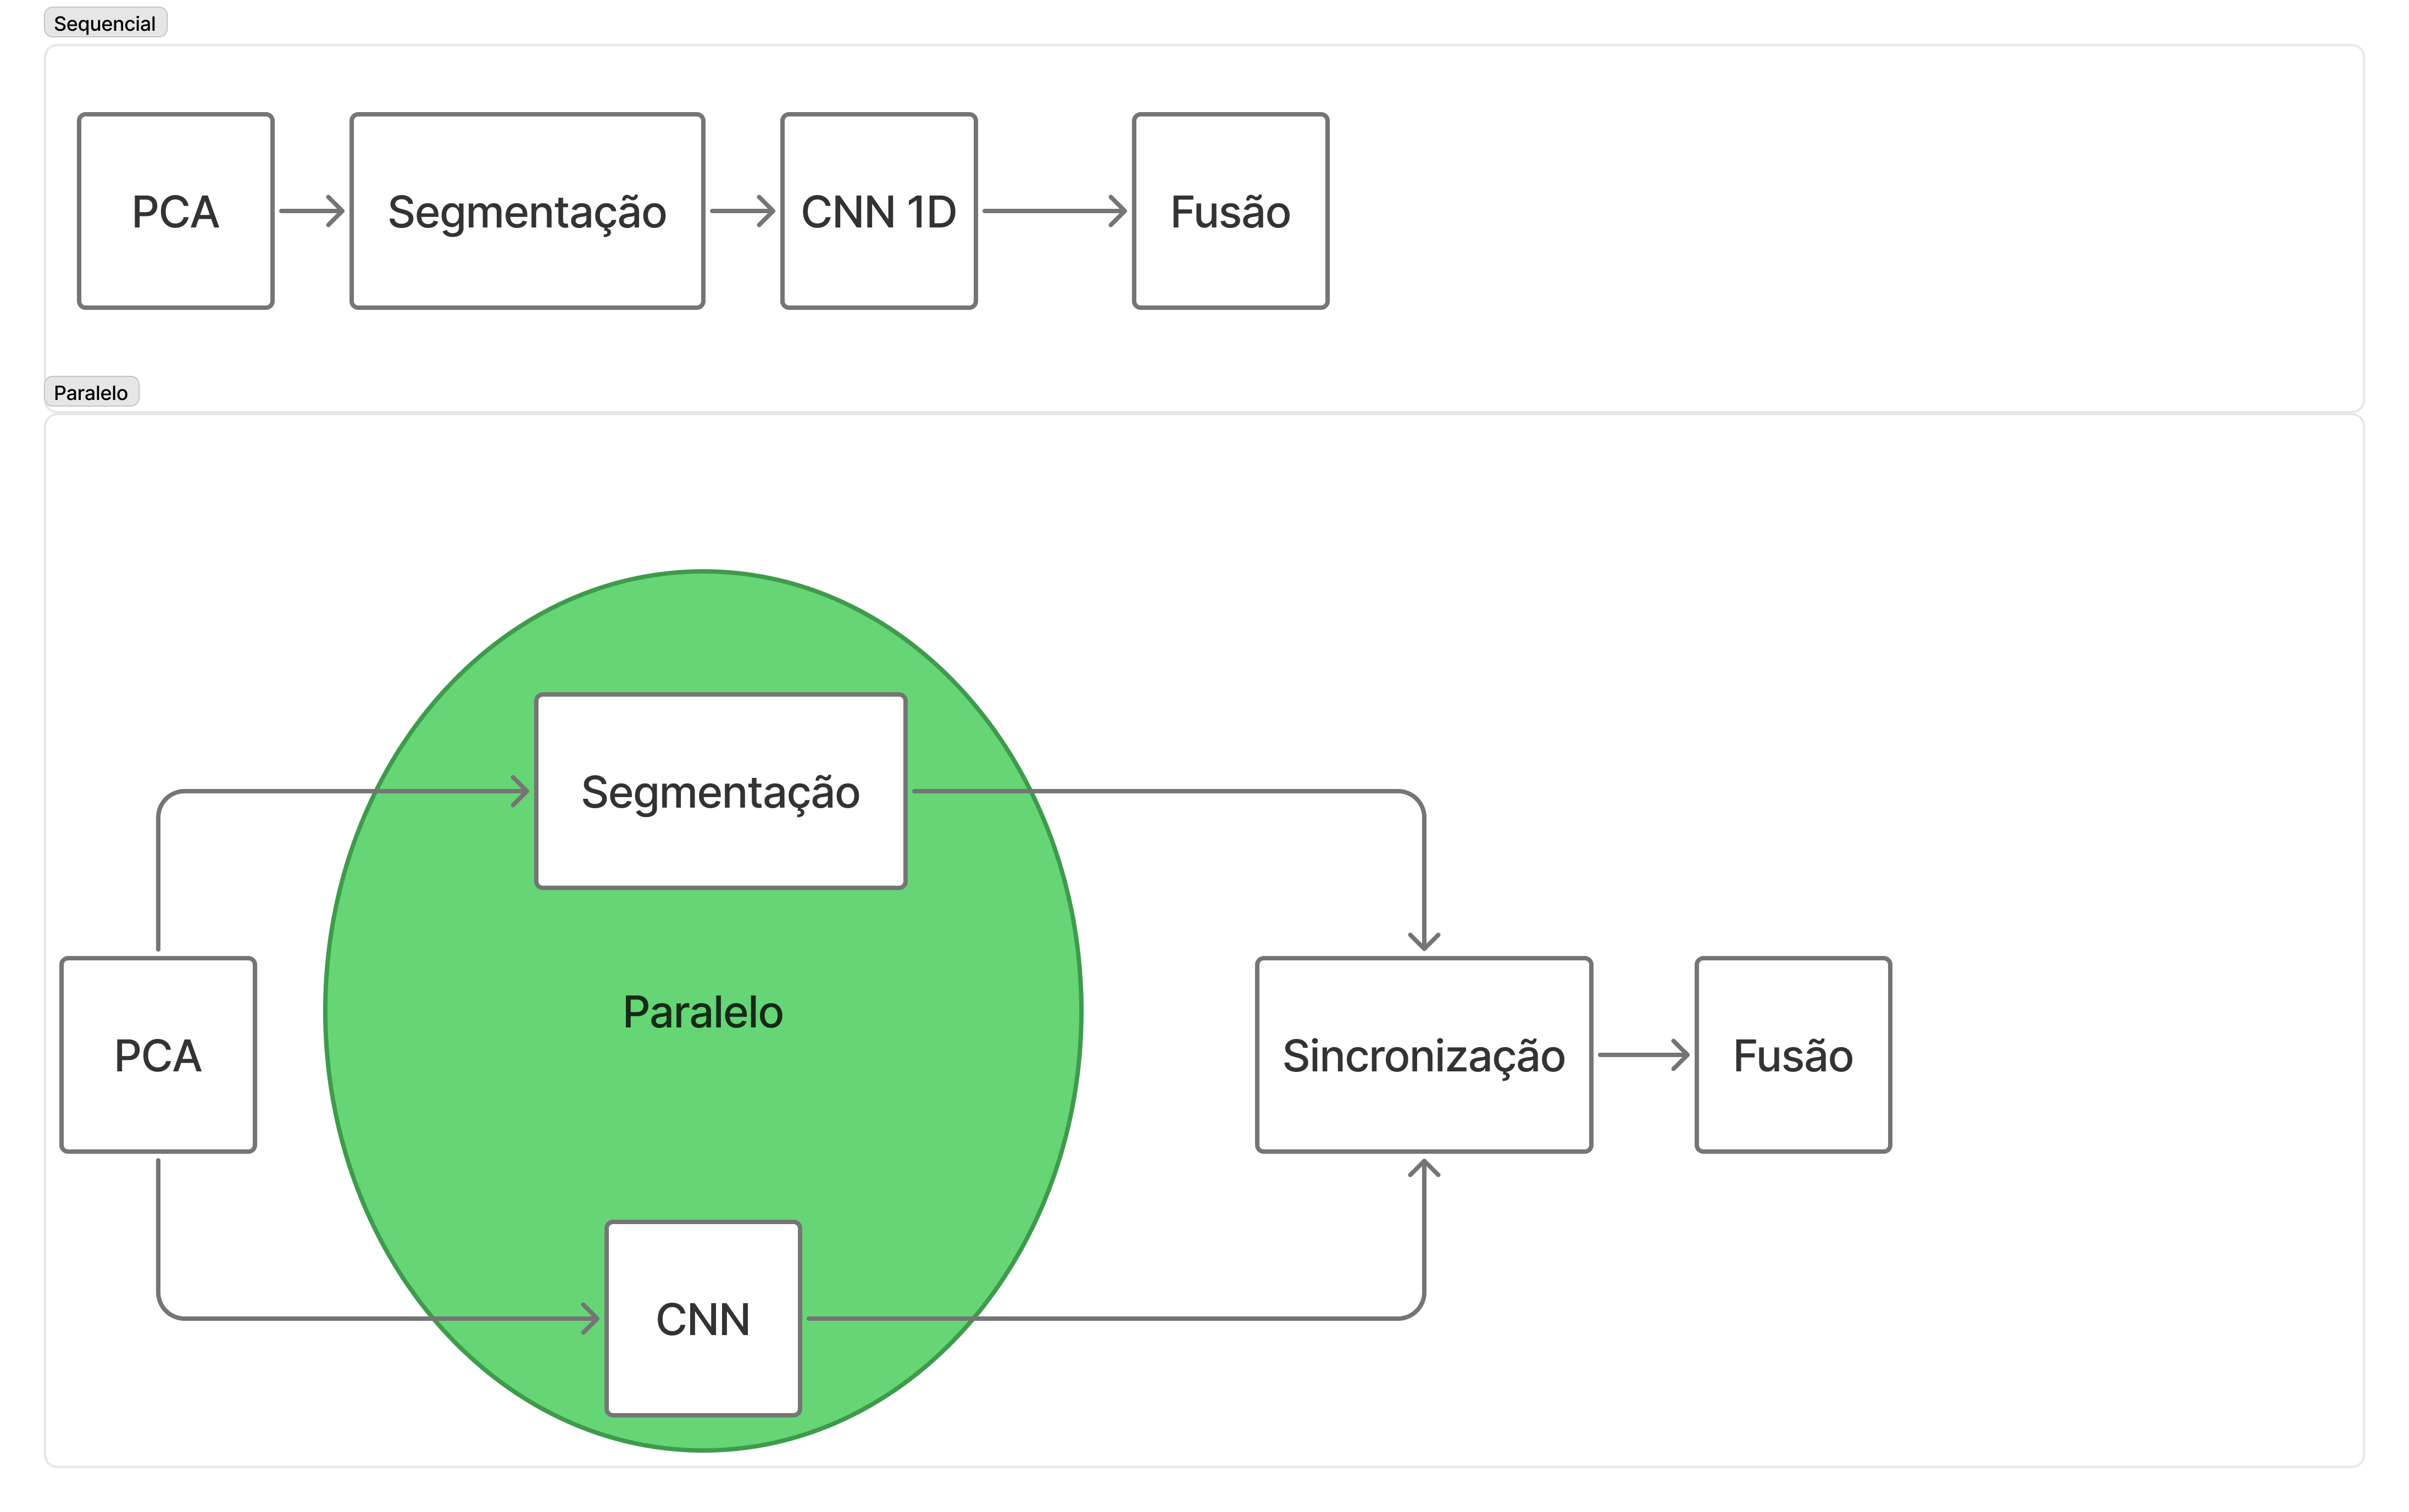
\includegraphics[width=0.7\textwidth]{src/assets/projeto/paralelizacao.png}\\
    \captionsetup{justification=raggedright}
    \caption*{Fonte: Elaborada pelo autor}
    \label{fig:paralelizacao}
\end{figure}

A Figura \ref{fig:paralelizacao} ilustra a diferença entre os dois fluxos de execução. No fluxo sequencial, após o PCA, a segmentação é executada primeiro, seguida pela CNN 1D, e então a fusão. No fluxo paralelo proposto, após o PCA, dois fluxos de execução são iniciados concorrentemente: um executa a segmentação espacial enquanto o outro executa a CNN 1D. O tempo esperado do fluxo paralelo é o maior entre os tempos das duas operações, acrescido da sobrecarga de coordenação (\autoref{sec:paralelismo}), de modo que o \textit{speedup} esperado é $(T_{seg} + T_{cnn}) / [\max(T_{seg}, T_{cnn}) + T_{overhead}]$, limitado pelo teto apresentado na \autoref{sec:concorrencia}. Por exemplo, se a segmentação levar 1 s e a CNN 3 s, o \textit{speedup} não passará de $4/3 \approx 1{,}33$; ele só se aproxima de 2 quando as duas etapas têm durações semelhantes.

\subsubsection{Otimização Automática de Hiperparâmetros}

Duas abordagens de otimização serão implementadas:

\textbf{Grid Search}: Busca exaustiva em um espaço discreto de hiperparâmetros. Para cada combinação possível de parâmetros, um modelo é treinado e avaliado. Apesar de custoso computacionalmente, garante exploração completa do espaço de busca definido \cite{liashchynskyi2019gridsearchrandomsearch}.

\textbf{Otimização Bayesiana}: Abordagem mais eficiente que modela a função objetivo (acurácia de validação) como um processo Gaussiano e utiliza uma função de aquisição para decidir quais configurações testar a seguir, balanceando exploração e explotação \cite{WU201926}.

Os hiperparâmetros a serem otimizados incluem:

\begin{itemize}
    \item \textbf{Para a CNN 1D}: taxa de aprendizado, tamanho do lote, número de épocas, taxa de \textit{dropout}, número de filtros por camada, tamanho dos \textit{kernels} e otimizador (Adam, SGD, RMSprop);
    \item \textbf{Para a segmentação}: número de superpixels, número de iterações e parâmetros específicos de cada algoritmo;
    \item \textbf{Para o PCA}: número de componentes principais.
\end{itemize}

\begin{figure}[H]
    \centering
    \captionsetup{justification=centering}
    \caption{Fluxo da otimização de hiperparâmetros}
    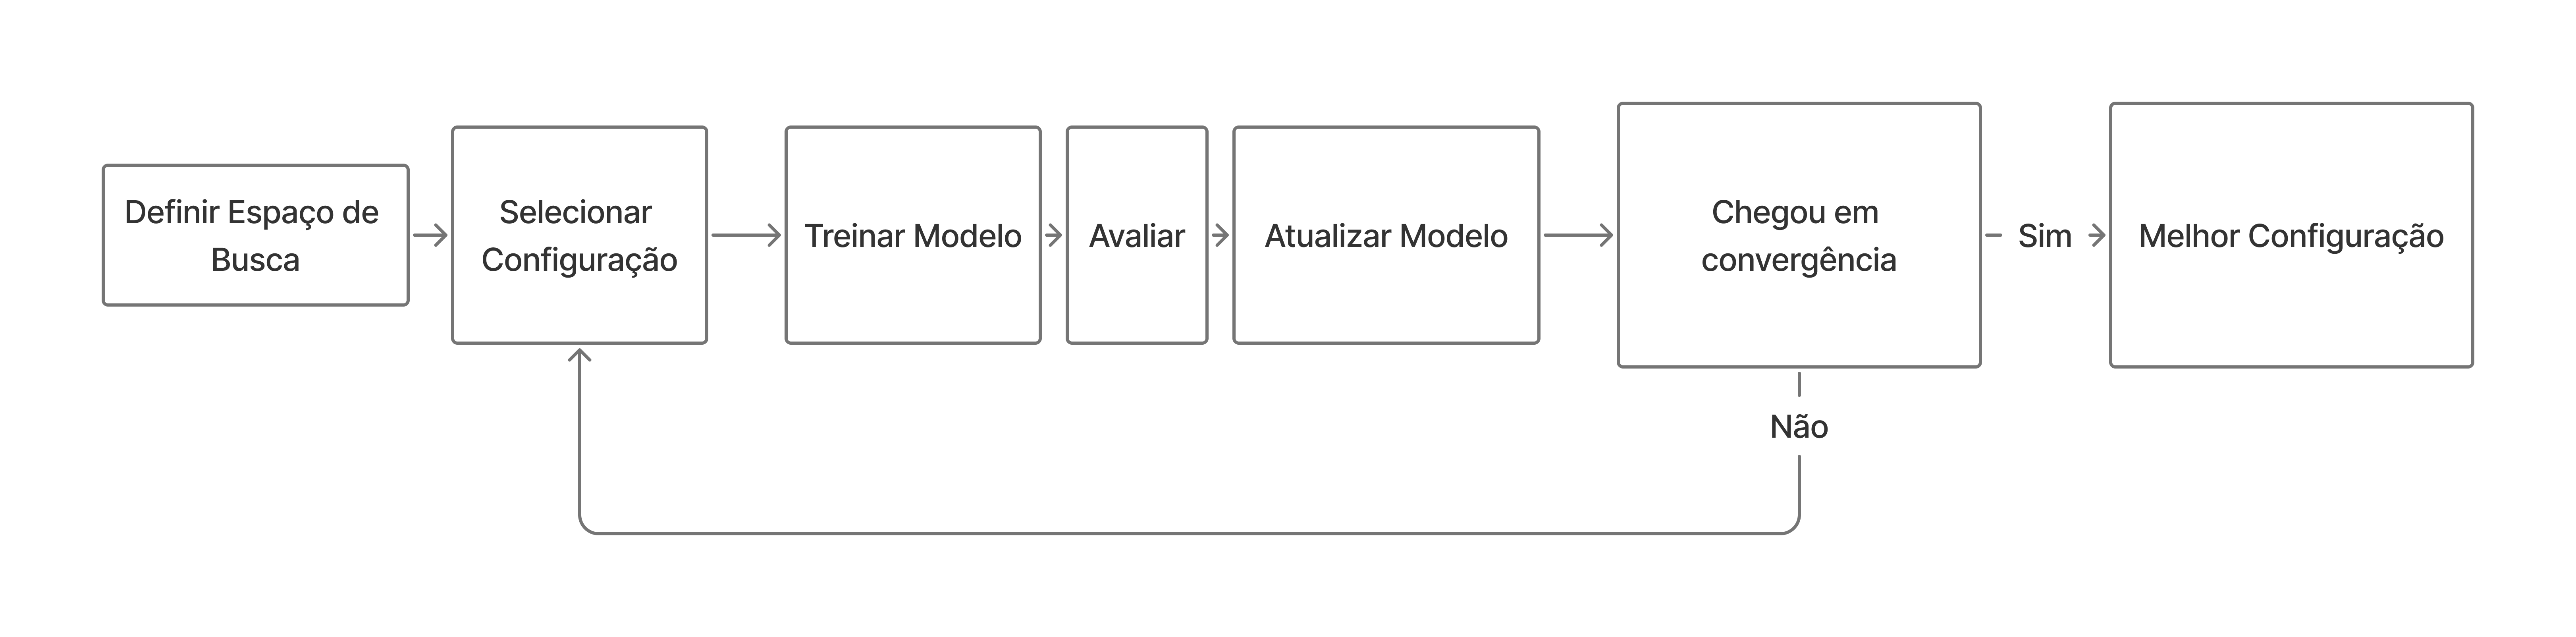
\includegraphics[width=0.7\textwidth]{src/assets/projeto/fluxoHPO.png}\\
    \captionsetup{justification=raggedright}
    \caption*{Fonte: Elaborada pelo autor}
    \label{fig:fluxoHPO}
\end{figure}

\section{Plano de Verificação}
\label{sec:planoVerificacao}

O plano de verificação estabelece um protocolo para validar o cumprimento dos requisitos estabelecidos e avaliar a eficácia das técnicas implementadas. A validação será conduzida através de uma campanha experimental, seguida de análise dos resultados obtidos. 

\subsection{Campanha Experimental}
\label{subsec:campanhaExperimental}

A campanha experimental será organizada de modo a garantir a comparabilidade dos resultados e permitir a análise incremental dos ganhos obtidos em cada etapa de otimização. A estratégia segue uma abordagem progressiva, em que cada experimento parte dos resultados do anterior, permitindo isolar e quantificar o impacto individual de cada técnica implementada.

Para cada dataset (Indian Pines, Salinas Valley e University of Pavia), serão realizados cinco experimentos principais, conforme detalhado no \autoref{tab:descricaoExperimentos}, o primeiro dos quais estabelece a linha de base.


\begin{quadro}[H]
    \centering
    \caption{Descrição detalhada dos experimentos}
    \begin{tabular}{|p{0.18\textwidth}|p{0.72\textwidth}|}
        \hline
        \rowcolor[HTML]{C0C0C0}
        \textbf{Experimento} & \textbf{Descrição} \\
        \hline
        
        \textbf{Exp. 1 - Baseline} & Reprodução da arquitetura original sem otimizações (CNN 1D + SEEDS com parâmetros fixos, processamento sequencial) para estabelecer linha de base \\
        \hline
        
        \textbf{Exp. 2 - Otimização de Segmentação} & Teste dos três algoritmos de segmentação (SEEDS, LSC, Watershed) com otimização automática de seus parâmetros, mantendo CNN fixa \\
        \hline
        
        \textbf{Exp. 3 - Otimização de CNN} & Otimização dos hiperparâmetros da CNN 1D mantendo segmentação fixa \\
        \hline
        
        \textbf{Exp. 4 - Otimização Conjunta} & Otimização simultânea dos hiperparâmetros de segmentação e CNN \\
        \hline
        
        \textbf{Exp. 5 - Paralelização} & Aplicação da estratégia de paralelização sobre a melhor configuração identificada \\
        \hline
    \end{tabular}
    \label{tab:descricaoExperimentos}
\end{quadro}

Para cada experimento, serão realizadas 5 execuções independentes com diferentes sementes aleatórias para avaliar a variabilidade dos resultados. As métricas coletadas serão:

\begin{itemize}
    \item Acurácia Geral (OA), Acurácia Média (AA), coeficiente Kappa
    \item Tempo de pré-processamento (PCA + Segmentação)
    \item Tempo de treinamento da CNN
    \item Tempo de inferência (total e por pixel)
    \item Uso de memória (pico durante treinamento e inferência)
    \item Número de parâmetros do modelo
    \item \textit{Speedup} obtido com paralelização
\end{itemize}

Os resultados serão organizados conforme \autoref{tab:planejamentoExperimentos}.

\begin{quadro}[H]
    \centering
    \caption{Planejamento de experimentos}
    \begin{tabular}{|p{0.20\textwidth}|p{0.12\textwidth}|p{0.15\textwidth}|p{0.12\textwidth}|p{0.12\textwidth}|p{0.12\textwidth}|}
        \hline
        \rowcolor[HTML]{C0C0C0}
        \textbf{Experimento} & \textbf{Dataset} & \textbf{Segmentação} & \textbf{HPO CNN} & \textbf{HPO Seg.} & \textbf{Paralelo} \\
        \hline
        
        Exp1 - Baseline & IP, SV, UP & SEEDS & - & - & - \\
        \hline
        
        Exp2 - Otim. Seg. & IP, SV, UP & SEEDS, LSC, WS & - & X & - \\
        \hline
        
        Exp3 - Otim. CNN & IP, SV, UP & SEEDS & X & - & - \\
        \hline
        
        Exp4 - Otim. Conjunta & IP, SV, UP & Melhor & X & X & - \\
        \hline
        
        Exp5 - Paralelização & IP, SV, UP & Melhor & X & X & X \\
        \hline
    \end{tabular}
    \label{tab:planejamentoExperimentos}
\end{quadro}

\subsection{Análise Estatística dos Resultados}

Para cada configuração, serão calculados a média e o desvio padrão de cada métrica entre as execuções com sementes diferentes, e a comparação entre configurações utilizará testes de significância estatística. O critério efetivamente adotado na execução, que substitui os testes por uma comparação com o desvio entre sementes, está registrado no \autoref{qua:desviosExperimentos}.

\subsection{Validação dos Requisitos}

A validação dos requisitos funcionais e não funcionais estabelecidos na \autoref{sec:req} será conduzida através de procedimentos específicos para cada requisito, conforme detalhado no \autoref{tab:planoVerificacaoRF} e no \autoref{tab:planoVerificacaoRNF}. Para cada requisito, são especificados os aspectos a serem validados, os métodos de validação a serem empregados e os critérios objetivos de sucesso.

\begin{quadro}[H]
    \centering
    \caption{Plano de verificação dos requisitos funcionais}
    \begin{tabular}{|p{0.08\textwidth}|p{0.25\textwidth}|p{0.35\textwidth}|p{0.22\textwidth}|}
        \hline
        \rowcolor[HTML]{C0C0C0}
        \textbf{Req.} & \textbf{Aspecto a Validar} & \textbf{Método de Validação} & \textbf{Critério de Sucesso} \\
        \hline
        
        \textbf{RF01} & Implementação correta da CNN 1D para extração de características espectrais & Testes verificando dimensões dos tensores em cada camada & Dimensões de saída de cada camada iguais às previstas na arquitetura \\
        \hline
        
        \textbf{RF02} & Implementação correta dos algoritmos de segmentação espacial & Testes verificando geração de mapas de superpixels & Mapas de segmentação gerados corretamente para os três algoritmos \\
        \hline
        
        \textbf{RF03} & Sistema de fusão por concatenação funcionando & Verificação das dimensões das características fusionadas correspondendo à soma das dimensões espectrais e espaciais & Fusão executada corretamente e classificação com fusão superior à classificação puramente espectral \\
        \hline
        
        \textbf{RF04} & Sistema de otimização automática de hiperparâmetros & Comparação entre algoritmos, verificando convergência e qualidade das configurações encontradas & OA da melhor configuração encontrada superior à da configuração de \citeonline{Souza2023}, nas mesmas condições de treino \\
        \hline
        
        \textbf{RF05} & Produção de métricas de desempenho e custo computacional & Coleta e registro de todas as métricas especificadas & Todas as métricas coletadas e registradas para análise comparativa \\
        \hline
        
        \textbf{RF06} & Eficácia da paralelização do processamento & Medição do tempo de execução com e sem paralelização, cálculo do \textit{speedup} obtido & \textit{Speedup} maior que 1 em relação ao fluxo sequencial, na mesma máquina \\
        \hline
    \end{tabular}
    \label{tab:planoVerificacaoRF}
\end{quadro}

\begin{quadro}[H]
    \centering
    \caption{Plano de verificação dos requisitos não funcionais}
    \begin{tabular}{|p{0.08\textwidth}|p{0.25\textwidth}|p{0.35\textwidth}|p{0.22\textwidth}|}
        \hline
        \rowcolor[HTML]{C0C0C0}
        \textbf{Req.} & \textbf{Aspecto a Validar} & \textbf{Método de Validação} & \textbf{Critério de Sucesso} \\
        \hline
        
        \textbf{RNF01} & Conformidade da arquitetura CNN 1D com o modelo base & Comparação estrutural com a arquitetura proposta por \cite{Souza2023} e \cite{Viel10064297} & Arquitetura implementada segue o modelo base especificado \\
        \hline
        
        \textbf{RNF02} & Desenvolvimento em Python & Verificação de que todos os módulos foram desenvolvidos em Python & Todos os módulos implementados em Python \\
        \hline
        
        \textbf{RNF03} & Utilização de plataforma adequada para treinamento & Confirmação de uso de Google Colab ou ambiente HPC com GPU & Experimentos executados em ambiente com aceleração por GPU \\
        \hline
        
        \textbf{RNF04} & Fusão por concatenação implementada corretamente & Verificação de que características espectrais e espaciais são concatenadas & Fusão realizada por concatenação de vetores \\
        \hline
        
        \textbf{RNF05} & Melhoria das métricas com otimização automática & Comparação das métricas OA, AA e Kappa entre configurações otimizadas automaticamente e ajuste manual & Métricas de acurácia superiores com otimização automática \\
        \hline
        
        \textbf{RNF06} & Reprodutibilidade dos resultados & Execução de múltiplas rodadas com mesmas configurações e análise de variabilidade & Desvio padrão das métricas inferior a 2\% entre execuções independentes \\
        \hline
        
        \textbf{RNF07} & Ganho de desempenho com paralelização & Medição quantitativa do \textit{speedup} obtido & \textit{Speedup} maior que 1 em relação à implementação sequencial, na mesma máquina \\
        \hline
    \end{tabular}
    \label{tab:planoVerificacaoRNF}
\end{quadro}

O \autoref{tab:validacaoDatasets} estabelece, para cada dataset, as metas de acurácia que o sistema otimizado deve atingir ou superar para ser considerado bem-sucedido. As metas são definidas neste projeto, e a comparação de referência é com os valores reportados por \citeonline{Souza2023} nas mesmas cenas: OA de 0,9142 em Indian Pines, 0,9965 em Salinas Valley e 0,9928 em University of Pavia. A meta de OA de Indian Pines fica, portanto, acima do valor reportado, e as de Salinas Valley e University of Pavia, abaixo.


\begin{quadro}[H]
    \centering
    \caption{Validação de desempenho nos datasets de referência}
    \resizebox{\textwidth}{!}{%
    \begin{tabular}{|p{0.18\textwidth}|p{0.28\textwidth}|p{0.28\textwidth}|p{0.20\textwidth}|}
        \hline
        \rowcolor[HTML]{C0C0C0}
        \textbf{Dataset} & \textbf{Aspecto a Validar} & \textbf{Método de Validação} & \textbf{Meta} \\
        \hline

        \textbf{Indian Pines} &
        Métricas OA, AA e Kappa iguais ou superiores às metas &
        Comparação com as metas e com os valores reportados por \citeonline{Souza2023} &
        $OA \geq 95\%$, $AA \geq 93\%$, $Kappa \geq 0{,}94$ \\
        \hline

        \textbf{Salinas Valley} &
        Métricas OA, AA e Kappa iguais ou superiores às metas &
        Comparação com as metas e com os valores reportados por \citeonline{Souza2023} &
        $OA \geq 97\%$, $AA \geq 96\%$, $Kappa \geq 0{,}96$ \\
        \hline

        \textbf{University of Pavia} &
        Métricas OA, AA e Kappa iguais ou superiores às metas &
        Comparação com as metas e com os valores reportados por \citeonline{Souza2023} &
        $OA \geq 98\%$, $AA \geq 97\%$, $Kappa \geq 0{,}97$ \\
        \hline
    \end{tabular}%
    }
    \label{tab:validacaoDatasets}
\end{quadro}

\section{Análise de Riscos} 
\label{sec:analiseRiscos}

A análise de riscos identifica potenciais problemas que podem impactar o desenvolvimento e execução do projeto, estabelecendo estratégias de mitigação para cada cenário.

O \autoref{tab:riscos} apresenta os principais riscos identificados, classificados quanto à probabilidade de ocorrência e ao impacto potencial no projeto. Nenhum risco foi classificado com probabilidade alta; o de maior impacto é o de o tempo de HPO exceder o cronograma, de probabilidade média e impacto alto.

\begin{quadro}[H]
    \centering
    \caption{Análise de riscos}
    \begin{tabular}{|p{0.22\textwidth}|p{0.12\textwidth}|p{0.10\textwidth}|p{0.46\textwidth}|}
        \hline
        \rowcolor[HTML]{C0C0C0}
        \textbf{Risco} & \textbf{Probab.} & \textbf{Impacto} & \textbf{Mitigação} \\
        \hline

        Tempo de HPO excede cronograma & Média & Alto & Reduzir espaço de busca e limitar número máximo de avaliações \\
        \hline

        Recursos computacionais insuficientes & Baixa & Médio & Utilizar Google Colab Pro e reduzir o tamanho do lote \\
        \hline

        Dificuldade de reproduzir baseline & Média & Médio & Contatar autores originais, ajustar hiperparâmetros cuidadosamente \\
        \hline

        Variabilidade alta nos resultados & Média & Médio & Aumentar o número de execuções e fixar as sementes aleatórias \\
        \hline
    \end{tabular}
    \label{tab:riscos}
\end{quadro}

\section{Cronograma}

O cronograma apresentado no \autoref{tab:cronograma} distribui as atividades do TCC ao longo do primeiro semestre de 2026. A escrita da monografia é uma atividade contínua. As implementações seguem ordem de dependências. Os experimentos são concentrados na segunda metade do período.

\begin{quadro}[H]
    \centering
    \caption{Cronograma de atividades do TCC}
    \begin{tabular}{|p{0.40\textwidth}|c|c|c|c|c|c|}
    \hline
    \rowcolor[HTML]{C0C0C0}
    \textbf{Atividade} & \textbf{Jan} & \textbf{Fev} & \textbf{Mar} & \textbf{Abr} & \textbf{Mai} & \textbf{Jun} \\
    \hline
    Escrita da Monografia & X & X & X & X & X & - \\
    \hline
    Implementação (CNN 1D, Segmentação, Fusão) & X & X & - & - & - & - \\
    \hline
    Implementação do Sistema de HPO & - & X & X & - & - & - \\
    \hline
    Implementação da Paralelização & - & - & X & - & - & - \\
    \hline
    Experimentos e Coleta de Métricas & - & - & X & X & X & - \\
    \hline
    Análise dos Resultados & - & - & - & - & X & X \\
    \hline
    Revisão Textual e Apresentação & - & - & - & X & X & X \\
    \hline
    \end{tabular}
    \label{tab:cronograma}
\end{quadro} \clearpage
\chapter{Desenvolvimento}
\label{cap:desenvolvimento}

Este capítulo descreve a implementação realizada a partir do projeto do \autoref{cap:proj}. Inicialmente são apresentados o ambiente e a organização do código, incluindo a reprodução da implementação original de \citeonline{Souza2023}, que é pré-requisito de todas as comparações. Na sequência, é descrito o fluxo de execução, do carregamento da cena às métricas. Em seguida, são apresentados os outros três eixos de otimização --- paralelismo, automação de hiperparâmetros e segmentadores ---, com destaque para a estratégia de fusão concorrente proposta pelo orientador. O capítulo termina com a organização dos experimentos e os desvios em relação ao projeto.

\section{Ambiente e Organização do Código}
\label{sec:ambiente}

\subsection{Ambiente de Execução}

A implementação foi desenvolvida em Python 3.12, com PyTorch 2.13 (CUDA 13.0) para a rede neural \cite{Paszke2019PyTorch}, scikit-learn para o PCA e as métricas, OpenCV para os algoritmos de segmentação e Optuna para a Otimização Bayesiana \cite{Akiba2019Optuna}. Os experimentos foram executados em um computador pessoal com GPU NVIDIA RTX 5070 Laptop, processador com 32 núcleos lógicos e 15,8 GB de memória RAM, sob WSL2. O ambiente virtual foi criado com o gerenciador \texttt{uv}, e as versões exatas de todas as bibliotecas ficam fixadas em um arquivo de requisitos versionado junto ao código e são conferidas ao iniciar o notebook.

\subsection{Organização em Pacote}

O trabalho de referência foi entregue como um notebook Jupyter, com estado global compartilhado entre células e configurações espalhadas pelo código. Para que cada resultado deste trabalho fosse atribuível a uma configuração conhecida, a implementação foi reorganizada em um pacote Python, com um módulo por responsabilidade e cada definição em um único lugar. O \autoref{qua:pacote} resume a organização. O notebook foi mantido, mas apenas importa o pacote e guarda a narrativa e as células de execução; os experimentos também integram o pacote, de modo que a implementação e as medições compartilham exatamente o mesmo código.

\begin{quadro}[H]
    \centering
    \caption{Organização do pacote da implementação}
    \begin{tabular}{|p{0.22\textwidth}|p{0.70\textwidth}|}
        \hline
        \rowcolor[HTML]{C0C0C0}
        \textbf{Módulo} & \textbf{Responsabilidade} \\
        \hline
        Configuração e ambiente & Parâmetros de uma execução em um único objeto imutável; seleção de dispositivo, sementes e modo determinístico \\
        \hline
        Dados & Carregamento das cenas, tabela de pixels, PCA, composição RGB, os quatro segmentadores e a divisão em treino, validação e teste \\
        \hline
        Modelo, treino e avaliação & CNN 1D com a fusão, laço de treino com parada antecipada e cálculo de OA, AA e Kappa \\
        \hline
        Pipeline & A única peça que conhece a ordem das etapas, chamada pelo notebook, pela busca de hiperparâmetros e pelos experimentos \\
        \hline
        Paralelismo & Execução concorrente dos ramos do pré-processamento, partição da cena e fusão concorrente \\
        \hline
        Hiperparâmetros & Espaço de busca, as três estratégias de busca, seleção dos vencedores e campanha final \\
        \hline
        MLOps & Registro imutável de cada execução, campanhas e relatórios \\
        \hline
        Visualização & Diagnósticos, explicabilidade e as figuras deste trabalho \\
        \hline
        Experimentos & Um módulo por experimento, com retomada a partir dos resultados já gravados \\
        \hline
    \end{tabular}
    \captionsetup{justification=raggedright}
    \caption*{Fonte: Elaborado pelo autor}
    \label{qua:pacote}
\end{quadro}

\subsection{Reprodução da Implementação Original}
\label{subsec:reproducao}

O notebook original foi escrito em TensorFlow/Keras, e a reimplementação foi feita em PyTorch. Antes de qualquer otimização, foi necessário garantir que a reimplementação fosse fiel ao original e que suas execuções se repetissem; sem isso, nenhuma diferença medida depois poderia ser atribuída à otimização. A reimplementação preserva a arquitetura do notebook --- 37.577 parâmetros em University of Pavia, idênticos aos do resumo do modelo Keras ---, o PCA com branqueamento, a divisão dos dados com as mesmas sementes do notebook (semente 42, com as mesmas 3.208 amostras de teste em University of Pavia) e os hiperparâmetros de treino: taxa de aprendizado 0,001, \textit{dropout} 0,5, lote 32 e teto de 60 épocas. A regra de parada antecipada foi trocada, como descrito na \autoref{subsec:desTreino}. Dois padrões do Keras precisaram ser replicados explicitamente, porque os do PyTorch são outros: a inicialização Xavier uniforme com viés nulo nas convoluções e nas camadas densas e o $\epsilon = 10^{-7}$ do otimizador Adam. O notebook original não fixa a semente da inicialização e do treino da rede, e a execução registrada nele obteve OA 0,9819, AA 0,9735 e Kappa 0,9760 em University of Pavia. Como os dois frameworks não partem dos mesmos pesos, a igualdade numérica com o Keras não é esperada: a equivalência é de arquitetura, de dados e de hiperparâmetros. A reimplementação, por sua vez, é determinística: com a configuração do notebook, execuções repetidas produzem o mesmo histórico de perda por época, os mesmos pesos finais e as mesmas métricas (OA 0,976309, AA 0,957918 e Kappa 0,968545).

A reprodutibilidade das execuções seguintes depende de três mecanismos. O primeiro é a configuração explícita: todos os parâmetros de uma execução ficam em um único objeto, que é gravado junto ao resultado e permite reconstruí-la. O segundo é o modo determinístico, que fixa as sementes do NumPy e do PyTorch, desativa a escolha automática de algoritmos do cuDNN e a precisão reduzida TF32, e restringe o OpenCV a uma única thread. Esta última restrição foi necessária porque o LSC paralelo do OpenCV devolvia rótulos diferentes a cada chamada, como discutido na \autoref{sec:resOrganizacao}. O terceiro é um contrato de dados verificado antes de cada treino: os conjuntos de treino, validação e teste precisam ser disjuntos, os espectros não podem conter valores inválidos, as classes precisam estar numeradas de forma contígua e as duas entradas da rede precisam ter uma linha por amostra.

Duas práticas de engenharia completam o eixo de organização. Cada \textit{trial} da busca de hiperparâmetros mantinha sua própria cópia dos dados preparados, embora dele só interessassem as métricas: 2,5 MB por \textit{trial} em Indian Pines, ou cerca de 450 MB em uma campanha de 180 \textit{trials}. Adotou-se, então, o ciclo de instanciar, treinar, extrair as métricas e liberar os recursos de cada \textit{trial}, de modo que apenas o melhor resultado corrente permanece em memória; com ele, a memória do processo cresceu 16 MB ao longo de uma campanha desse tamanho (\autoref{sec:resOrganizacao}). Além disso, toda execução longa tornou-se retomável: os resultados são gravados a cada configuração concluída de um experimento, e uma execução interrompida continua de onde parou, relendo o que já foi medido.

\section{Fluxo de Execução}
\label{sec:fluxo}

Uma execução completa percorre as etapas a seguir, sempre na mesma ordem:

\begin{enumerate}
    \item \textbf{Carregamento da cena}: o cubo hiperespectral $(H, W, B)$ e o mapa de verdade terrestre $(H, W)$ são lidos e achatados em uma tabela de $H \cdot W$ pixels;
    \item \textbf{Ramo espectral}: os pixels sem rótulo (\textit{background}) são removidos e o PCA com branqueamento (\textit{whitening}) reduz as $B$ bandas a $K_b$ componentes (30 em Indian Pines e 15 em University of Pavia e Salinas Valley, como no original);
    \item \textbf{Ramo espacial}: um PCA de 3 componentes sobre a cena inteira, incluindo o \textit{background}, gera uma composição RGB de 8 bits, que o segmentador divide em superpixels; o identificador da região de cada pixel rotulado é a segunda entrada da rede;
    \item \textbf{Divisão dos dados}: as amostras são divididas em treino, validação e teste e, opcionalmente, o treino é subamostrado;
    \item \textbf{Treino}: a CNN 1D é construída e treinada com parada antecipada;
    \item \textbf{Avaliação}: o modelo treinado classifica o conjunto de teste, e OA, AA, Kappa e a matriz de confusão são calculados.
\end{enumerate}

Os dois ramos são independentes até o ponto de fusão. É essa independência que as estratégias de paralelismo da \autoref{sec:desParalelismo} exploram.

\subsection{Segmentadores}
\label{subsec:desSegmentadores}

Os quatro segmentadores --- SEEDS, SLIC (no modo SLICO), LSC e Watershed --- são implementados sobre o OpenCV e devolvem saídas no mesmo formato: o mapa de rótulos $(H, W)$ e a máscara de contornos. Por isso, trocar o segmentador não altera nenhuma outra etapa. O Watershed do OpenCV não fornece a máscara de contornos, que é então derivada do mapa de rótulos, e recebe marcadores dispostos em uma grade regular; as linhas que ele marca entre bacias foram mantidas como uma região própria.

Os parâmetros de cada algoritmo são definidos por cena (\autoref{qua:paramSeg}). Indian Pines usa regiões menores, porque tem apenas 145 $\times$ 145 pixels e classes agrícolas em faixas estreitas (\autoref{fig:indian_pines}). O número de superpixels pedido ao SEEDS é um alvo, não uma garantia: em Indian Pines, 350 superpixels pedidos resultam em 81 regiões; em University of Pavia, 150 resultam em 45.

\begin{quadro}[H]
    \centering
    \caption{Parâmetros padrão dos segmentadores por cena}
    \begin{tabular}{|p{0.16\textwidth}|p{0.38\textwidth}|p{0.36\textwidth}|}
        \hline
        \rowcolor[HTML]{C0C0C0}
        \textbf{Algoritmo} & \textbf{Indian Pines} & \textbf{University of Pavia e}\newline\textbf{Salinas Valley} \\
        \hline
        SEEDS & 350 superpixels, 200 iterações, \textit{prior} 2, 10 níveis, 5 \textit{bins} de histograma & 150 superpixels, 150 iterações, \textit{prior} 1, 8 níveis, 15 \textit{bins} \\
        \hline
        SLIC & região de 8 px, 10 iterações & região de 12 px, 10 iterações \\
        \hline
        LSC & região de 8 px, razão 0,075, 10 iterações & região de 12 px, razão 0,075, 10 iterações \\
        \hline
        Watershed & 350 marcadores & 500 marcadores \\
        \hline
    \end{tabular}
    \captionsetup{justification=raggedright}
    \caption*{Fonte: Elaborado pelo autor. Os valores do SEEDS são os do notebook original de \citeonline{Souza2023}; o texto daquele trabalho relata 150 superpixels em Indian Pines e, em University of Pavia e Salinas Valley, \textit{prior} 2 e 3 níveis}
    \label{qua:paramSeg}
\end{quadro}

\subsection{Modelo e Fusão}
\label{subsec:desModelo}

A CNN 1D segue o notebook original e está detalhada no \autoref{qua:camadas} para Indian Pines. As quatro convoluções não usam preenchimento (\textit{padding}), e cada uma encurta a sequência em $k - 1$ posições, consumindo 14 posições no total; por isso a rede exige pelo menos 15 componentes espectrais. Em University of Pavia e Salinas Valley, com 15 componentes, a última convolução produz uma única posição, e o achatamento resulta em 64 características.

\begin{quadro}[H]
    \centering
    \caption{Camadas da CNN 1D com fusão, em Indian Pines ($K_b = 30$)}
    \begin{tabular}{|p{0.36\textwidth}|p{0.30\textwidth}|p{0.18\textwidth}|}
        \hline
        \rowcolor[HTML]{C0C0C0}
        \textbf{Camada} & \textbf{Saída}\newline\textbf{(canais, comprimento)} & \textbf{Parâmetros} \\
        \hline
        Entrada: espectro após PCA & (1, 30) & --- \\
        \hline
        Conv1D 16 filtros, $k = 9$, ReLU & (16, 22) & 160 \\
        \hline
        Conv1D 32 filtros, $k = 3$, ReLU & (32, 20) & 1.568 \\
        \hline
        Conv1D 64 filtros, $k = 3$, ReLU & (64, 18) & 6.208 \\
        \hline
        Conv1D 64 filtros, $k = 3$, ReLU & (64, 16) & 12.352 \\
        \hline
        Achatamento & 1.024 & --- \\
        \hline
        Fusão: concatenação do identificador do superpixel & 1.025 & --- \\
        \hline
        Densa 128, ReLU, \textit{dropout} & 128 & 131.328 \\
        \hline
        Densa 64, ReLU, \textit{dropout} & 64 & 8.256 \\
        \hline
        Densa de saída (\textit{logits}) & 16 & 1.040 \\
        \hline
        \textbf{Total} & & \textbf{160.912} \\
        \hline
    \end{tabular}
    \captionsetup{justification=raggedright}
    \caption*{Fonte: Elaborado pelo autor}
    \label{qua:camadas}
\end{quadro}

A fusão é tardia: as convoluções nunca veem o identificador do superpixel, que só é concatenado ao vetor de características depois do achatamento, como um número a mais. A cabeça densa é a única parte da rede que enxerga as duas informações juntas. Na implementação, a concatenação foi separada da cabeça densa em um passo próprio, o que permite à fusão concorrente da \autoref{subsec:fusaoConcorrente} proteger apenas esse passo com uma trava. Como alternativa à concatenação do identificador numérico, também foi implementada uma tabela de vetores aprendidos por região (\textit{embedding}), usada apenas para entender como o identificador é aproveitado pela rede; a configuração herdada, com o identificador numérico, é a referência de todas as comparações.

\subsection{Treino, Parada Antecipada e Divisão dos Dados}
\label{subsec:desTreino}

O treino usa a perda de entropia cruzada e o otimizador Adam. A parada antecipada segue uma política explícita: o treino é interrompido após 10 épocas sem que a acurácia de validação melhore em pelo menos 0,001, e os pesos da melhor época são restaurados. Nos experimentos de segmentadores e de hiperparâmetros (05, 06, 08 e 10; \autoref{qua:experimentos}), há ainda uma meta: o treino é interrompido quando a acurácia de validação atinge 0,95, com os pesos da melhor época igualmente restaurados, e o teto é de 200 épocas (no experimento 08, orçamentos de 10, 40 e 200 épocas por \textit{trial}). Nos experimentos de partição (11 e 13) e na fusão concorrente (14), vale apenas a paciência, com teto de 25 e de 60 épocas, respectivamente; o teto de 60 épocas é o do notebook original. O original, porém, parava pela perda de validação, com paciência de 5 épocas; a troca para a acurácia de validação foi feita para que a mesma métrica governe a parada e a seleção de hiperparâmetros. Em todos os casos, a escolha de modelos e de hiperparâmetros usa exclusivamente o conjunto de validação, e as métricas de teste são apenas relatadas.

A divisão dos dados reproduz a do original: um sorteio estratificado por classe separa 85\% das amostras para treino e divide os 15\% restantes igualmente entre validação e teste. Opcionalmente, apenas uma fração do treino é usada, com amostragem estratificada; validação e teste permanecem intactos, para que as métricas continuem comparáveis entre frações. Os experimentos de segmentadores e de hiperparâmetros (05, 06, 08 e 10) usam 10\% do treino, tanto na busca quanto no retreino do vencedor; os demais usam o treino completo.

\section{Paralelismo}
\label{sec:desParalelismo}

Três estratégias de paralelismo foram implementadas, em níveis diferentes do fluxo. A primeira executa concorrentemente os dois ramos do pré-processamento; a segunda divide a cena em partes processadas ao mesmo tempo; a terceira sobrepõe a segmentação à extração de características da rede. O paralelismo muda quando cada passo é executado, e não o que ele calcula, e os experimentos de partição e de fusão concorrente conferem isso: na partição da cena, a OA das execuções em processos foi igual à da execução sequencial das mesmas partições em todos os valores de $N$ medidos; na fusão concorrente, as 723 execuções do experimento 14 previram as mesmas classes que a inferência em um único lote (\autoref{subsec:resFusao}). A exceção é o treino independente das partições em threads: as partições compartilham o gerador de números aleatórios do PyTorch, consumido em ordem imprevisível na inicialização dos pesos e nas máscaras de \textit{dropout}, e execuções idênticas variaram até 3,51 pontos de OA (\autoref{sec:resOrganizacao}). Com processos, cada partição tem o seu gerador, e o resultado se repete.

\subsection{Entre os Ramos do Pré-processamento}

A preparação dos dados pode executar os ramos espectral e espacial de três formas: em sequência, que é a linha de base; em duas threads, que compartilham os \textit{arrays} de entrada sem cópia; ou com o ramo espacial em um processo filho, que exige serializar a tabela de pixels e os resultados. A versão com threads funciona apesar do GIL porque a maior parte do processamento dos dois ramos ocorre em código nativo que libera o GIL: a álgebra linear do PCA e a iteração do segmentador no OpenCV. Pelo segundo corolário da \autoref{sec:concorrencia}, o ganho máximo é dado pelos tempos dos dois ramos, e o ramo espacial, que contém a segmentação, é o mais longo, com 78\% a 93\% do tempo sequencial do pré-processamento (\autoref{qua:ramos}).

\subsection{Por Partição da Cena}

Para paralelizar a etapa mais custosa do fluxo, o treino, a cena é dividida em $N$ partições com número semelhante de pixels rotulados, de modo que o teto teórico do \textit{speedup} se aproxime de $N$. A segmentação é executada uma única vez sobre a cena inteira, antes da partição: segmentar cada parte separadamente produziria superpixels diferentes nas fronteiras, e os identificadores deixariam de ser comparáveis entre partições. As partições são faixas horizontais contíguas, e dois modos de uso foram implementados: o \textit{replicado}, em que um único modelo é treinado com a cena inteira e apenas a inferência é paralelizada, e o \textit{independente}, em que cada partição treina seu próprio modelo com as amostras dela. Nos experimentos de partição, o treino usa lote 64, em vez dos 32 da receita herdada, e o \textit{speedup} é medido contra a execução sequencial das mesmas partições, no mesmo dispositivo. Como o lote é o mesmo nos dois lados da comparação, o \textit{speedup} compara executores sob a mesma carga, mas as acurácias desses experimentos não são comparáveis às da linha de base.

As partições podem ser executadas em sequência, em threads ou em processos. Os processos são criados pelo método \textit{spawn}, que inicia um novo interpretador, sem herdar o estado do processo pai, porque o PyTorch interrompe com erro a cópia de processo (\textit{fork}) feita depois que o cálculo de gradientes foi executado em threads \cite{PyTorchMultiprocessing}. O custo do \textit{spawn} é alto, porque cada processo reimporta o PyTorch: com 16 partições, a partida chega a 78\% do tempo de uma execução com o pool criado dentro da medição (\autoref{qua:poolQuente}). Por isso, foi implementado um pool reutilizável: os processos são criados e aquecidos uma única vez, fora da medição, e atendem às execuções seguintes. Cada processo é configurado para usar uma única thread do PyTorch, pois, do contrário, $N$ processos com 16 threads cada disputariam os mesmos núcleos. Antes de criar um pool, a memória necessária é estimada a partir da memória ocupada por processo, cerca de 481 MB, e um pool que não caberia na RAM é recusado em vez de levar o sistema a usar a área de troca.

\subsection{Fusão Concorrente}
\label{subsec:fusaoConcorrente}

O projeto previa que a segmentação e a CNN 1D fossem executadas ao mesmo tempo, com sincronização apenas no ponto de fusão (\autoref{fig:paralelizacao}). A estratégia de paralelismo entre os ramos, porém, executou concorrentemente à segmentação apenas o PCA espectral; a CNN só era executada depois. O orientador deste trabalho detalhou, então, um esquema que cumpre a proposta original, representado na \autoref{fig:fusaoConcorrente}:

\begin{itemize}
    \item uma thread T0 executa o ramo espacial --- PCA de 3 componentes, composição RGB e SEEDS --- e publica o mapa de segmentação (MS) em uma estrutura compartilhada;
    \item um pool de threads T1 a TN recebe as posições do mapa: cada tarefa passa o espectro dos pixels daquelas posições apenas pelas convoluções da rede, lê o identificador do segmento de cada posição no mapa e faz a concatenação, e a cabeça densa produz o vetor de classes;
    \item a segmentação e a concatenação são protegidas por um mutex.
\end{itemize}

\begin{figure}[H]
    \centering
    \captionsetup{justification=centering}
    \caption{Fusão concorrente: T0 segmenta enquanto o pool T1 a TN extrai as características e realiza a fusão}
    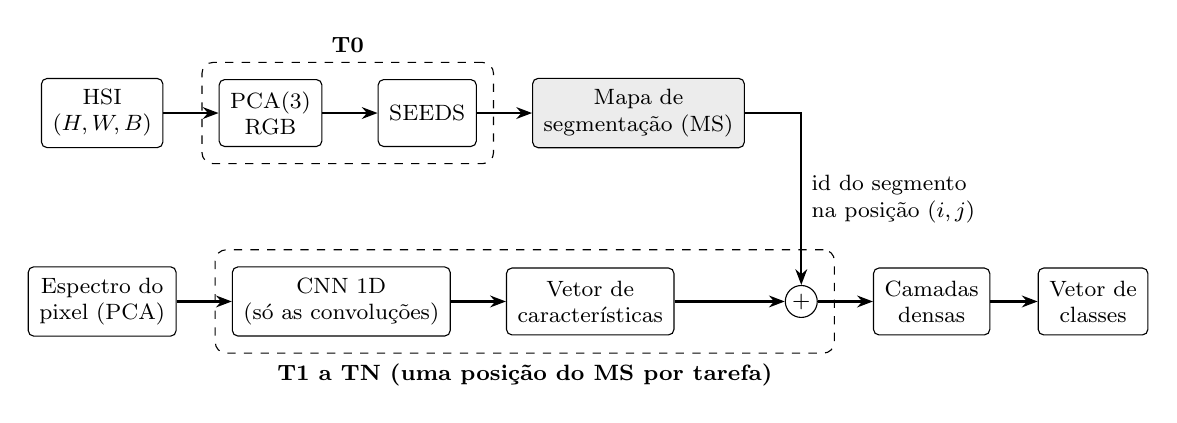
\begin{tikzpicture}[
        font=\footnotesize,
        caixa/.style={draw, rounded corners=2pt, minimum height=0.85cm, align=center, inner sep=4pt},
        thread/.style={draw, dashed, rounded corners=4pt, inner sep=6pt},
        seta/.style={-{Stealth[length=2mm]}, thick}
    ]
        \node[caixa] (hsi) {HSI\\$(H, W, B)$};
        \node[caixa, right=0.7cm of hsi] (pca3) {PCA(3)\\RGB};
        \node[caixa, right=0.7cm of pca3] (seeds) {SEEDS};
        \node[caixa, right=0.7cm of seeds, fill=gray!15] (ms) {Mapa de\\segmentação (MS)};
        \node[thread, fit=(pca3)(seeds), label={[font=\footnotesize\bfseries]above:T0}] (t0) {};

        \node[caixa, below=1.5cm of hsi] (pix) {Espectro do\\pixel (PCA)};
        \node[caixa, right=0.7cm of pix] (conv) {CNN 1D\\(só as convoluções)};
        \node[caixa, right=0.7cm of conv] (vet) {Vetor de\\características};
        \node[circle, draw, right=1.4cm of vet, inner sep=1pt] (cat) {$+$};
        \node[caixa, right=0.7cm of cat] (dens) {Camadas\\densas};
        \node[caixa, right=0.6cm of dens] (cls) {Vetor de\\classes};
        \node[thread, fit=(conv)(vet)(cat), label={[font=\footnotesize\bfseries]below:T1 a TN (uma posição do MS por tarefa)}] (tn) {};

        \draw[seta] (hsi) -- (pca3);
        \draw[seta] (pca3) -- (seeds);
        \draw[seta] (seeds) -- (ms);
        \draw[seta] (pix) -- (conv);
        \draw[seta] (conv) -- (vet);
        \draw[seta] (vet) -- (cat);
        \draw[seta] (ms.east) -| node[pos=0.75, right, align=left]{id do segmento\\na posição $(i, j)$} (cat.north);
        \draw[seta] (cat) -- (dens);
        \draw[seta] (dens) -- (cls);
    \end{tikzpicture}
    \captionsetup{justification=raggedright}
    \caption*{Fonte: Elaborada pelo autor, a partir do esquema proposto pelo orientador}
    \label{fig:fusaoConcorrente}
\end{figure}

As convoluções não dependem do mapa de segmentação, e é isso que permite às threads de trabalho avançar enquanto T0 ainda segmenta: só a concatenação precisa esperar. Duas decisões de implementação foram necessárias para transformar o esquema em um programa correto.

A primeira diz respeito à ordem. Um mutex garante que T0 e as threads de trabalho não acessem o mapa ao mesmo tempo, mas não garante que T0 o acesse primeiro: se uma thread de trabalho adquirir a trava antes de T0, lerá um mapa ainda vazio. Por isso, a trava do esquema foi implementada como a de uma variável de condição (\autoref{sec:concorrencia}), cujo predicado é um indicador de que o mapa já foi publicado. Uma thread que chega antes da publicação aguarda, liberando a trava durante a espera, e T0, ao publicar o mapa, notifica todas as threads bloqueadas. Para tornar visível qualquer leitura indevida, o mapa começa preenchido com um valor que nenhum segmentador produz.

A segunda diz respeito à extensão da seção crítica. Foram implementadas duas versões, comparáveis porque todo o resto é idêntico:

\begin{itemize}
    \item \textbf{como no esquema}: T0 detém a trava durante toda a segmentação, e cada tarefa a detém durante a concatenação;
    \item \textbf{mínima}: T0 adquire a trava apenas para publicar o mapa pronto, e cada tarefa, apenas para ler os identificadores. Depois de publicado, o mapa passa a ser somente lido, e leituras concorrentes de um dado imutável não produzem condição de corrida; manter a concatenação dentro da trava serializa as threads sem proteger nada.
\end{itemize}

A granularidade das tarefas também é um parâmetro, medido com blocos de 1, 64 e 1.024 posições. Com um bloco de uma posição, cada tarefa recebe um único pixel, exatamente como no esquema; com blocos maiores, cada tarefa recebe um conjunto contíguo de posições, o que dilui o custo fixo de despachar uma tarefa e de chamar a rede. Esse custo pesa: em Indian Pines, chamar a rede pixel a pixel, mesmo sem threads, já torna a inferência 3,12 vezes mais lenta que a de todos os pixels em um único lote, e com uma posição por tarefa o esquema fica de 7 a 35 vezes mais lento (\autoref{subsec:resFusao}).

Na implementação do esquema, cada tarefa faz as convoluções e a fusão em sequência; é a forma chamada de \textit{como no esquema} no \autoref{qua:fusao}, na \autoref{fig:fusaoSpeedup} e na \autoref{fig:fusaoLinhaTempo}. Isso tem uma consequência estrutural: uma thread que termina as convoluções antes de T0 publicar o mapa fica bloqueada à espera dele e, enquanto isso, não atende nenhuma outra tarefa da fila. Enquanto T0 segmenta, portanto, no máximo $N$ tarefas avançam, e a sobreposição pretendida fica limitada a $N$ vezes o tamanho do bloco. Para medir o teto do esquema, foi implementada também uma \textit{variante desacoplada}, em que convolução e fusão são tarefas separadas e todas as convoluções entram na fila antes de qualquer fusão. Como a fila do pool é atendida em ordem de chegada, quando uma fusão é retirada da fila, a convolução correspondente já foi iniciada, e nenhuma thread fica ociosa enquanto ainda há convolução a fazer. As duas extensões da seção crítica foram medidas nas duas formas.

Três cuidados completam a implementação. O modo de cálculo de gradientes do PyTorch é definido por thread; por isso, a inferência sem gradientes precisa ser ativada dentro de cada tarefa, e não apenas na thread principal. Pelo mesmo motivo, o número de threads internas do PyTorch, que nas medições de paralelismo é restrito a uma, precisa ser fixado em cada thread do pool: a configuração feita na thread principal não se propaga, e as threads do pool usariam as 32 threads padrão do OpenMP, o que fazia a convolução de um bloco de 64 pixels levar cerca de 100 ms em vez de 0,2 ms. Por fim, as threads do pool são criadas sob demanda e inicializam estado interno do PyTorch na primeira operação; o pool é, então, aquecido antes das medições com uma barreira que obriga a criação de todas as threads, separando o custo de partida do custo do paralelismo, como no pool de processos.

O esquema se aplica à propagação direta (\textit{forward pass}) de um modelo já treinado, isto é, à inferência. No treino, a perda de cada lote depende do identificador do segmento desde o primeiro lote, e o gradiente atravessa as convoluções; além disso, a segmentação é executada uma única vez. Não há, portanto, trabalho de treino que possa ser sobreposto à segmentação.

\section{Automação de Hiperparâmetros}
\label{sec:desHPO}

O espaço de busca combina os hiperparâmetros de treino, o número de componentes do PCA, o segmentador e três receitas de parâmetros de cada segmentador (\autoref{qua:espaco}). Os valores de cada hiperparâmetro incluem o da receita herdada, de modo que a configuração original é um dos candidatos possíveis. Em Indian Pines o espaço tem $4 \times 3 \times 3^4 \times 3 = 2.916$ combinações. Com o tempo médio de treino de um \textit{trial} do experimento 08 com teto de 200 épocas (3,2 s, com 10\% do treino), percorrê-las levaria cerca de 2,6 h de treino por semente, 146 vezes o custo de uma busca de 20 \textit{trials}, e a comparação das estratégias repete cada busca com 3 sementes. Por isso, a busca em grade prevista no projeto foi substituída pela busca aleatória, que, assim como a grade, não usa os resultados anteriores para escolher o próximo candidato e é a referência usual para avaliar estratégias adaptativas \cite{Bergstra2012Random}.

\begin{quadro}[!htbp]
    \centering
    \caption{Espaço de busca de hiperparâmetros}
    \begin{tabular}{|p{0.28\textwidth}|>{\RaggedRight\arraybackslash}p{0.40\textwidth}|>{\RaggedRight\arraybackslash}p{0.20\textwidth}|}
        \hline
        \rowcolor[HTML]{C0C0C0}
        \textbf{Hiperparâmetro} & \textbf{Valores} & \textbf{Herdado} \\
        \hline
        Taxa de aprendizado & 0,0003; 0,001; 0,003 & 0,001 \\
        \hline
        \textit{Dropout} & 0,20; 0,35; 0,50 & 0,50 \\
        \hline
        \textit{Weight decay} & 0; $10^{-5}$; $10^{-4}$ & 0 \\
        \hline
        Tamanho do lote & 32; 64; 128 & 32 \\
        \hline
        Componentes do PCA & 0,5$\times$, 1$\times$ e 1,5$\times$ o valor da cena, com mínimo de 15 (Indian Pines: 15, 30, 45; University of Pavia e Salinas Valley: 15, 22) & 30 (Indian Pines), 15 (University of Pavia e Salinas Valley) \\
        \hline
        Segmentador & SEEDS, SLIC, LSC, Watershed & SEEDS \\
        \hline
        Receita do segmentador & a padrão e duas variações em torno dela: no SEEDS, 0,7$\times$ e 1,35$\times$ o número de superpixels, com 120 e 250 iterações e \textit{prior} 1 e 3; no SLIC, o tamanho da região $\pm$3 px; no LSC, o tamanho da região $\pm$3 px, com razão 0,04 e 0,12; no Watershed, 0,7$\times$ e 1,35$\times$ o número de marcadores & a padrão \\
        \hline
    \end{tabular}
    \captionsetup{justification=raggedright}
    \caption*{Fonte: Elaborado pelo autor}
    \label{qua:espaco}
\end{quadro}

Todo candidato é representado da mesma forma: uma lista de índices, um por hiperparâmetro. Essa representação é comum às três estratégias implementadas, o que garante que elas difiram apenas na forma de escolher o próximo candidato:

\begin{itemize}
    \item \textbf{busca aleatória}: sorteia os índices de forma uniforme, sem repetir candidatos;
    \item \textbf{TPE}: usa o amostrador da biblioteca Optuna, tratando segmentador e receita como hiperparâmetros categóricos e os demais como inteiros ordenados \cite{Bergstra2011TPE, Akiba2019Optuna};
    \item \textbf{algoritmo genético}: população de 6 candidatos no experimento de comparação das estratégias, seleção por torneio entre 3, cruzamento uniforme, mutação de cada gene com probabilidade de 0,25 e elitismo dos 2 melhores, que passam à geração seguinte sem novo treino \cite{Holland1975}.
\end{itemize}

As três estratégias começam com a mesma cobertura: os quatro primeiros \textit{trials} são obrigados a usar segmentadores distintos, para que nenhum fique de fora da busca por acaso. Cada \textit{trial} é avaliado pela maior acurácia de validação de seu histórico. Na busca de baixa fidelidade, a paciência da parada antecipada passa a ser um terço do orçamento de épocas quando esse valor é menor que 10, para que ainda possa ser acionada: com 10 épocas por \textit{trial}, ela cai para 3; com 40 e com 200 épocas, permanece 10. Ao final da busca, apenas o vencedor é retreinado, com teto de 200 épocas e 5 sementes (experimentos 06 e 10), e a decisão --- o que foi buscado, o que venceu e o plano final --- é gravada em arquivos com \textit{hash}, de modo que seja possível justificar posteriormente a promoção de cada receita.

\section{Segmentadores sob Otimização Conjunta}
\label{sec:desSegmentadores}

O plano de verificação previa testar os segmentadores mantendo a CNN fixa. Esse desenho foi implementado e descartado (\autoref{cap:resultados}): a configuração da CNN que serve a um segmentador não serve a outro, e a comparação com a CNN fixa mede quanto uma receita arbitrária combina com cada algoritmo, e não a qualidade do algoritmo. No uso real, a CNN e o segmentador são ajustados juntos, e a comparação foi refeita dessa forma: para cada segmentador, uma busca TPE de 16 \textit{trials}, restrita a ele, cujo vencedor, escolhido pela acurácia de validação, é retreinado com 5 sementes. O SEEDS passa pelo mesmo tratamento e é a referência.

\section{Organização dos Experimentos}
\label{sec:desExperimentos}

A campanha planejada no \autoref{tab:descricaoExperimentos} foi desdobrada em experimentos menores, cada um com um objetivo específico, conforme o \autoref{qua:experimentos}. A numeração segue a ordem em que foram criados; os números ausentes correspondem a experimentos absorvidos por outros, descartados quando o escopo foi restrito à CNN 1D, ou não abordados nesta monografia. Cada experimento é executável a partir de um lançador de linha de comando, grava seus resultados em arquivos tabulares versionados e confere, quando aplicável, a repetibilidade das próprias medições.

\begin{quadro}[H]
    \centering
    \caption{Experimentos realizados e correspondência com o plano de verificação}
    \begin{tabular}{|p{0.07\textwidth}|p{0.46\textwidth}|p{0.19\textwidth}|p{0.16\textwidth}|}
        \hline
        \rowcolor[HTML]{C0C0C0}
        \textbf{Exp.} & \textbf{Objetivo} & \textbf{Eixo} & \textbf{Plano} \\
        \hline
        05 & Comparação dos segmentadores com a CNN fixa & Segmentadores & Exp. 2 (contraexemplo) \\
        \hline
        06 & Comparação dos segmentadores, cada um com hiperparâmetros otimizados & Segmentadores & Exp. 2 e 4 \\
        \hline
        08 & Comparação entre busca aleatória, TPE e algoritmo genético; efeito do orçamento de épocas; importância de cada hiperparâmetro & Hiperparâmetros & Exp. 3 e 4 \\
        \hline
        10 & Receita otimizada em comparação com a herdada & Hiperparâmetros & Exp. 1, 3 e 4 \\
        \hline
        11 & Escalabilidade da partição da cena, nos modos replicado e independente & Paralelismo & Exp. 5 \\
        \hline
        13 & Pool frio em comparação com pool quente & Paralelismo & Exp. 5 \\
        \hline
        14 & Fusão concorrente & Paralelismo & Exp. 5 \\
        \hline
    \end{tabular}
    \captionsetup{justification=raggedright}
    \caption*{Fonte: Elaborado pelo autor}
    \label{qua:experimentos}
\end{quadro}

\section{Desvios em Relação ao Projeto}
\label{sec:desvios}

A implementação manteve os requisitos do projeto, mas algumas escolhas mudaram ao longo do desenvolvimento. O \autoref{qua:desvios} reúne as que dizem respeito à implementação, e o \autoref{qua:desviosExperimentos}, as que dizem respeito à campanha experimental, cada uma com o seu motivo.

\begin{quadro}[H]
    \centering
    \caption{Desvios em relação ao projeto: implementação}
    \begin{tabular}{|>{\RaggedRight\arraybackslash}p{0.27\textwidth}|>{\RaggedRight\arraybackslash}p{0.27\textwidth}|>{\RaggedRight\arraybackslash}p{0.36\textwidth}|}
        \hline
        \rowcolor[HTML]{C0C0C0}
        \textbf{Previsto} & \textbf{Realizado} & \textbf{Motivo} \\
        \hline
        TensorFlow/Keras ou PyTorch & PyTorch & Arquitetura, PCA, divisão dos dados e hiperparâmetros de treino do original preservados em PyTorch, com execução determinística; a regra de parada antecipada foi trocada (última linha deste quadro) \\
        \hline
        CNN com 16, 32, 64 e 128 filtros, \textit{max-pooling} e \textit{softmax} & 16, 32, 64 e 64 filtros, sem \textit{pooling}, saída em \textit{logits} & A arquitetura do notebook original, que é a referência; o \textit{softmax} é aplicado pela função de perda \\
        \hline
        Rótulo do superpixel codificado em \textit{one-hot} & Identificador numérico concatenado, como no original & A configuração herdada é a referência; o \textit{embedding} foi implementado para análise \\
        \hline
        Critério do RF03: classificação com fusão superior à puramente espectral & Fusão verificada pela concatenação e pela dimensão da entrada da cabeça densa (1.025 em Indian Pines); a vantagem sobre a rede puramente espectral é a reportada por \citeonline{Souza2023} & A fusão faz parte da configuração de referência e não é variável de estudo; nenhuma configuração sem fusão é treinada \\
        \hline
        SEEDS, LSC e Watershed & SEEDS, SLIC, LSC e Watershed & O SLIC é uma referência frequente nas avaliações de algoritmos de superpixels \cite{Stutz2018} e uma comparação natural \\
        \hline
        Busca em grade e Otimização Bayesiana com Ray Tune & Busca aleatória, TPE (Optuna) e algoritmo genético & As 2.916 combinações custariam 146 vezes uma busca de 20 \textit{trials} (\autoref{sec:desHPO}); o genético acrescenta uma estratégia populacional \\
        \hline
        Épocas, filtros, tamanho dos \textit{kernels} e otimizador entre os hiperparâmetros da CNN & Taxa de aprendizado, \textit{dropout}, \textit{weight decay} e lote; arquitetura e otimizador Adam fixos & A arquitetura e o otimizador são os do original, que é a referência; o orçamento de épocas foi estudado à parte, no experimento 08 \\
        \hline
        Google Colab ou HPC & GPU local (RTX 5070 Laptop) & Suficiente para as três cenas, com controle total do ambiente; os 15,8 GB de RAM impediram o pool de 32 processos (\autoref{sec:resParalelismo}) \\
        \hline
        Parada do notebook original: perda de validação, paciência 5 & Acurácia de validação, paciência 10, melhores pesos restaurados; meta de 0,95 nos experimentos de segmentadores e de hiperparâmetros & A mesma métrica governa a parada e a seleção \\
        \hline
    \end{tabular}
    \captionsetup{justification=raggedright}
    \caption*{Fonte: Elaborado pelo autor}
    \label{qua:desvios}
\end{quadro}

\begin{quadro}[H]
    \centering
    \caption{Desvios em relação ao projeto: campanha experimental}
    \begin{tabular}{|>{\RaggedRight\arraybackslash}p{0.27\textwidth}|>{\RaggedRight\arraybackslash}p{0.27\textwidth}|>{\RaggedRight\arraybackslash}p{0.36\textwidth}|}
        \hline
        \rowcolor[HTML]{C0C0C0}
        \textbf{Previsto} & \textbf{Realizado} & \textbf{Motivo} \\
        \hline
        Segmentadores com CNN fixa & Segmentadores sob otimização conjunta & O desenho com CNN fixa se mostrou inválido (\autoref{cap:resultados}) \\
        \hline
        85\% das amostras para treino & 10\% desse treino nos experimentos de segmentadores e de hiperparâmetros & Cada execução fica cerca de 5,7 vezes mais barata em Indian Pines (\autoref{qua:fracaoTreino}), o que viabilizou os 540 \textit{trials} do experimento 08; validação e teste permanecem inteiros \\
        \hline
        Todos os experimentos nas três cenas & CNN fixa (05) em Indian Pines e University of Pavia; segmentadores (06) e fusão concorrente (14) nas três; busca (08), ganho da busca de hiperparâmetros (10) e partição (11 e 13) em Indian Pines & Custo de tempo; Indian Pines é a cena de menor acurácia na linha de base (OA 0,9051; \autoref{qua:linhaBase}) \\
        \hline
        Testes de significância estatística & Diferença afirmável quando excede duas vezes o desvio combinado das duas condições entre sementes & Com 3 a 5 sementes por condição, um critério simples e explícito; por usar o desvio das execuções, e não o erro padrão da média, é mais exigente que o mesmo limiar aplicado ao erro padrão; o pareamento por semente não foi explorado \\
        \hline
        Segmentação em processo e CNN na GPU, em paralelo & Threads e processos em CPU, em três níveis & Em Indian Pines, o pré-processamento é 0,9\% de uma execução e a inferência, 0,4\% (\autoref{sec:resParalelismo}); o tempo concentra-se no treino, e a comparação entre executores exige o mesmo dispositivo \\
        \hline
        Paralelização sobre a melhor configuração identificada & Fusão concorrente sobre a configuração herdada; partição com lote 64 e 25 épocas & Interessa o tempo entre executores, com a mesma configuração dos dois lados \\
        \hline
    \end{tabular}
    \captionsetup{justification=raggedright}
    \caption*{Fonte: Elaborado pelo autor}
    \label{qua:desviosExperimentos}
\end{quadro}
 \clearpage
\chapter{Resultados}
\label{cap:resultados}

Este capítulo descreve primeiro o protocolo de execução e a linha de base, obtida com a configuração do trabalho de \citeonline{Souza2023}. Em seguida, os resultados da campanha experimental são organizados pelos quatro eixos de otimização: organização do código, paralelismo, automação de hiperparâmetros e segmentadores. O capítulo termina com a verificação dos requisitos e a discussão dos resultados.

\section{Protocolo de Execução}
\label{sec:resProtocolo}

Todos os experimentos foram executados no ambiente descrito na \autoref{sec:ambiente}, em modo determinístico. Salvo a comparação com o trabalho original (\autoref{qua:linhaBase}) e as acurácias citadas nas medições de paralelismo, obtidas com uma única semente (42), os resultados de acurácia são médias de execuções com sementes distintas (5 sementes nos retreinos finais e 3 nas comparações de estratégias de busca, na fração do treino e na análise do identificador) e, onde o desvio foi registrado, são apresentados com o desvio padrão populacional entre elas. Os tempos são médias de repetições da mesma configuração; nas medições de paralelismo em CPU, o PyTorch foi restrito a uma thread interna, salvo onde indicado, para que $N$ threads ou processos de trabalho correspondessem a $N$ núcleos, e os pools foram criados e aquecidos fora do intervalo medido, com o custo de partida registrado à parte.

Os experimentos de hiperparâmetros e de segmentadores treinam com 10\% do conjunto de treino (871 amostras em Indian Pines), com teto de 200 épocas, parada por estagnação de 10 épocas e meta de acurácia de validação de 0,95; a validação e o teste permanecem inteiros. Treinar com essa fração torna cada \textit{trial} 5,7 vezes mais barato (6,0 s contra 34,3 s por execução em Indian Pines; \autoref{qua:fracaoTreino}); o ganho da busca com o treino completo não foi medido. O custo dessa redução em acurácia, medido com a configuração herdada, está na \autoref{sec:resLinhaBase}. Os demais experimentos usam o treino completo.

\section{Linha de Base}
\label{sec:resLinhaBase}

Com a configuração do próprio notebook, a reimplementação obtém em University of Pavia OA 0,9763, AA 0,9579 e Kappa 0,9685, e repete esses valores, o histórico de perda por época e os pesos finais em execuções sucessivas. A execução registrada no notebook original, que não fixa a semente da inicialização e do treino da rede, obteve OA 0,9819, AA 0,9735 e Kappa 0,9760. Os dois frameworks não partem dos mesmos pesos, de modo que a igualdade numérica não é esperada, e uma diferença de 0,56 ponto na OA entre uma execução de cada lado não permite separar o efeito da implementação do efeito da inicialização. O que sustenta as comparações seguintes é que a reimplementação preserva a arquitetura (37.577 parâmetros nessa cena, os mesmos do modelo Keras), o PCA, a divisão dos dados, com as mesmas sementes e as mesmas 3.208 amostras de teste, e os hiperparâmetros de treino, e que cada configuração produz sempre o mesmo resultado; nas comparações seguintes, só a regra de parada antecipada difere da do original (\autoref{subsec:desTreino}).

O \autoref{qua:linhaBase} compara a configuração herdada, executada pela reimplementação com a política de parada da \autoref{subsec:desTreino} e o treino completo, com os valores reportados por \citeonline{Souza2023}. Os valores do trabalho original são superiores --- por menos de 1 ponto de OA em Indian Pines e Salinas Valley, 1,6 ponto em University of Pavia e 7,2 pontos de AA em Indian Pines, onde as classes raras pesam mais ---, o que é coerente com o modo como foram obtidos: o autor relata ter ajustado, por conjunto de dados, a paciência da parada antecipada e outros parâmetros de treino ao buscar o melhor resultado \cite{Souza2023}, enquanto aqui a mesma política vale para as três cenas. A comparação é entre uma execução de cada lado, com a semente 42 na reimplementação.

\begin{quadro}[H]
    \centering
    \caption{Configuração herdada: valores reportados no trabalho original e obtidos pela reimplementação}
    \begin{tabular}{|p{0.20\textwidth}|c|c|c|c|c|c|}
        \hline
        \rowcolor[HTML]{C0C0C0}
        & \multicolumn{3}{c|}{\textbf{Reportado}} & \multicolumn{3}{c|}{\textbf{Reimplementação}} \\
        \hline
        \rowcolor[HTML]{C0C0C0}
        \textbf{Cena} & \textbf{OA} & \textbf{AA} & \textbf{Kappa} & \textbf{OA} & \textbf{AA} & \textbf{Kappa} \\
        \hline
        Indian Pines & 0,9142 & 0,8956 & 0,9019 & 0,9051 & 0,8237 & 0,8914 \\
        \hline
        University of Pavia & 0,9928 & 0,9866 & 0,9905 & 0,9772 & 0,9644 & 0,9698 \\
        \hline
        Salinas Valley & 0,9965 & 0,9970 & 0,9962 & 0,9938 & 0,9956 & 0,9931 \\
        \hline
    \end{tabular}
    \captionsetup{justification=raggedright}
    \caption*{Fonte: Elaborado pelo autor, com os valores reportados por \citeonline{Souza2023}. Reimplementação: semente 42, treino completo}
    \label{qua:linhaBase}
\end{quadro}

O \autoref{qua:fracaoTreino} mostra o custo de treinar com menos amostras, medido em Indian Pines com a configuração herdada. Com 10\% do treino, a OA cai 14,3 pontos percentuais e a AA, 23,0, enquanto o tempo por execução cai de 34,3 s para 6,0 s. Os resultados com 10\% do treino, portanto, não são comparáveis em valor absoluto aos do \autoref{qua:linhaBase}; são comparáveis entre si, porque todas as condições comparadas em cada experimento usam a mesma fração.

\begin{quadro}[H]
    \centering
    \caption{Custo de treinar com uma fração do conjunto de treino (Indian Pines, 3 sementes, teto de 60 épocas)}
    \begin{tabular}{|c|c|c|c|c|c|}
        \hline
        \rowcolor[HTML]{C0C0C0}
        \textbf{Fração} & \textbf{Amostras} & \textbf{OA} & \textbf{AA} & \textbf{Kappa} & \textbf{Tempo (s)} \\
        \hline
        100\% & 8.711 & 0,9016 $\pm$ 0,0016 & 0,8308 & 0,8877 & 34,3 \\
        \hline
        50\% & 4.356 & 0,8643 $\pm$ 0,0140 & 0,7310 & 0,8448 & 18,8 \\
        \hline
        25\% & 2.179 & 0,8270 $\pm$ 0,0105 & 0,6755 & 0,8021 & 11,4 \\
        \hline
        10\% & 871 & 0,7586 $\pm$ 0,0109 & 0,6006 & 0,7227 & 6,0 \\
        \hline
        5\% & 435 & 0,6810 $\pm$ 0,0131 & 0,5322 & 0,6334 & 4,0 \\
        \hline
    \end{tabular}
    \captionsetup{justification=raggedright}
    \caption*{Fonte: Elaborado pelo autor}
    \label{qua:fracaoTreino}
\end{quadro}

\section{Organização do Código}
\label{sec:resOrganizacao}

O principal resultado deste eixo é qualitativo: a reimplementação fiel à arquitetura, ao PCA, à divisão dos dados e aos hiperparâmetros de treino do original, com a regra de parada antecipada trocada (\autoref{subsec:desTreino}), e a reprodutibilidade das execuções, em que a mesma configuração produz sempre o mesmo resultado. A organização, porém, também tornou visíveis três defeitos: dois que teriam contaminado resultados em silêncio e um que interrompia a campanha com um erro que não apontava a causa.

\textbf{Não determinismo do LSC.} A implementação paralela do LSC no OpenCV desempata pela ordem das threads, e duas chamadas com a mesma imagem e os mesmos parâmetros devolviam rótulos diferentes em 388 pixels de Indian Pines; SEEDS, SLIC e Watershed não tinham o problema. Com o LSC no espaço de busca, a pontuação de um mesmo \textit{trial} variava entre execuções, e as estratégias adaptativas amplificavam a variação até trocarem de vencedor: a mesma campanha de TPE chegou a 0,8713 de validação em uma execução e a 0,7711 em outra, na qual, com 200 épocas por \textit{trial}, ficou atrás da busca aleatória (0,8075) e do algoritmo genético (0,8309). O defeito foi isolado por eliminação --- treino com configuração fixa determinístico, amostradores determinísticos com pontuações fixas e, por fim, a comparação direta das saídas dos segmentadores --- e corrigido restringindo o OpenCV a uma thread, com custo nulo (38,6 ms por segmentação, contra 39,1 ms com 32 threads). As medições anteriores à correção que envolviam o LSC foram descartadas, exceto três, assinaladas: o LSC sob otimização conjunta (\autoref{qua:segmentadores}), o LSC com a CNN fixa em University of Pavia e as métricas estruturais do LSC no \autoref{qua:estruturaSeg}.

\textbf{Gerador aleatório compartilhado entre threads.} Quando as partições da cena treinam em threads de um mesmo processo, todas consomem o mesmo gerador aleatório global do PyTorch, na inicialização dos pesos e nas máscaras de \textit{dropout}, em ordem imprevisível. Execuções que deveriam ser idênticas variaram até 3,51 pontos de OA, enquanto as execuções sequenciais e em processos repetiram o valor exatamente. Não há semente que corrija isso sem dar um gerador a cada partição, que é o que processos fazem por construção; por isso, toda acurácia de partição reportada vem de execuções sequenciais ou em processos.

\textbf{Número mínimo de componentes.} A geração das opções de PCA do espaço de busca usava um piso herdado da composição RGB (3 componentes), e não o da rede, que exige 15. Em University of Pavia e Salinas Valley, cuja receita é de 15 componentes, a busca gerava a opção de 8, e o primeiro \textit{trial} que a sorteava interrompia a campanha com um erro do PyTorch que apontava para a convolução, e não para a causa. O piso passou a ser derivado dos próprios \textit{kernels} da rede.

Quanto à memória, cada \textit{trial} da busca retinha 2,5 MB em Indian Pines, 5,1 MB em University of Pavia e 6,5 MB em Salinas Valley. Com a liberação dos resultados que não são o melhor corrente, a memória do processo cresceu 16 MB ao longo de uma campanha de 180 \textit{trials} (de 1.894 MB para 1.910 MB). Na CNN 1D, cujo conjunto de dados é pequeno, reter todos os resultados seria incômodo, mas não impeditivo (cerca de 450 MB em 180 \textit{trials} de Indian Pines); a liberação serve para manter constante a memória da campanha.

\section{Paralelismo}
\label{sec:resParalelismo}

\subsection{Entre os Ramos do Pré-processamento}

O \autoref{qua:ramos} e a \autoref{fig:ramos} mostram o tempo de cada ramo e o ganho de executá-los concorrentemente. A segmentação domina o pré-processamento (de 78\% a 93\% do tempo serial) e, pelo teto da \autoref{sec:concorrencia}, o ganho máximo fica entre 1,08$\times$ e 1,29$\times$. Com threads, Salinas Valley atinge 1,22$\times$ contra um teto de 1,21$\times$, ou seja, a implementação está no limite do que o desenho permite; em Indian Pines, o ganho fica em 1,05$\times$, contra um teto de 1,29$\times$, e em University of Pavia, onde o teto é 1,08$\times$, a sobrecarga de coordenação já basta para anular o ganho (0,95$\times$). Com processos, o custo de criar o processo filho e serializar de 8,4 MB a 45,3 MB de dados faz o pré-processamento ficar de 1,3 a 4,5 vezes mais lento.

\begin{quadro}[H]
    \centering
    \caption{Paralelismo entre os ramos do pré-processamento (5 repetições, tempos em segundos)}
    \begin{tabular}{|l|c|c|c|c|c|c|}
        \hline
        \rowcolor[HTML]{C0C0C0}
        \textbf{Cena} & \textbf{Espectral} & \textbf{Espacial} & \textbf{Sequencial} & \textbf{Threads} & \textbf{Processos} & \textbf{Teto} \\
        \hline
        Indian Pines & 0,037 & 0,129 & 0,166 & 1,05$\times$ & 0,22$\times$ & 1,29$\times$ \\
        \hline
        University of Pavia & 0,072 & 0,899 & 0,971 & 0,95$\times$ & 0,75$\times$ & 1,08$\times$ \\
        \hline
        Salinas Valley & 0,142 & 0,680 & 0,822 & 1,22$\times$ & 0,74$\times$ & 1,21$\times$ \\
        \hline
    \end{tabular}
    \captionsetup{justification=raggedright}
    \caption*{Fonte: Elaborado pelo autor. Teto: tempo sequencial dividido pelo tempo do ramo espacial. Como o teto é calculado com tempos médios, uma medição pode ficar ligeiramente acima dele, como em Salinas Valley}
    \label{qua:ramos}
\end{quadro}

\begin{figure}[H]
    \centering
    \captionsetup{justification=centering}
    \caption{Tempo de cada ramo do pré-processamento e \textit{speedup} medido contra o teto teórico}
    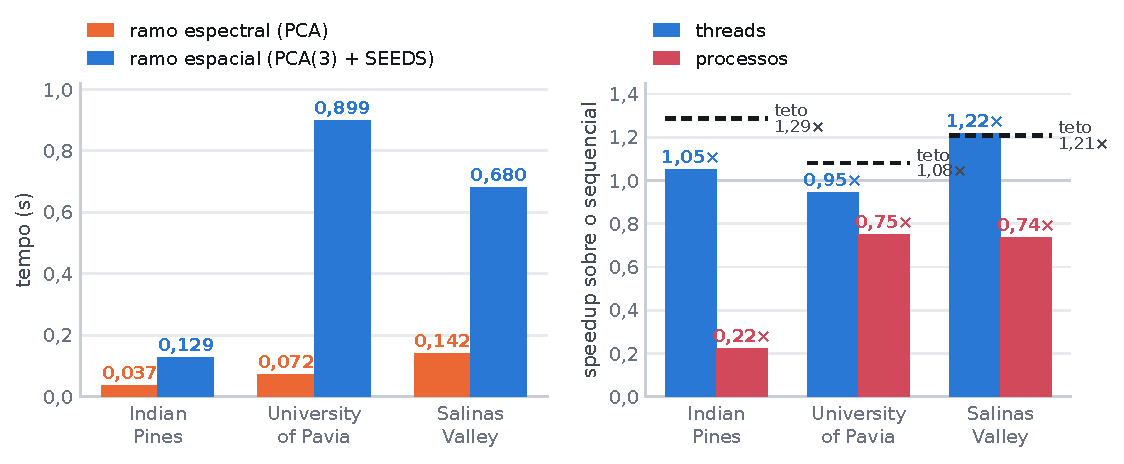
\includegraphics[width=\textwidth]{assets/resultados/ramos_preprocessamento.pdf}
    \captionsetup{justification=raggedright}
    \caption*{Fonte: Elaborada pelo autor}
    \label{fig:ramos}
\end{figure}

Há, porém, um limite mais forte que o teto dos ramos. Em Indian Pines, o pré-processamento inteiro leva 0,193~s, contra 20,13~s de treino, e representa 0,9\% do tempo de uma execução; pela lei de Amdahl, nenhuma otimização dele muda o tempo total em mais de 0,9\%. Esse resultado motivou a partição da cena, que paraleliza o treino, etapa que concentra o tempo de execução; a fusão concorrente, apresentada depois, atua sobre a segmentação e a inferência.

\subsection{Threads Internas do PyTorch}

Antes de paralelizar o treino entre partições, foi medido o paralelismo que o próprio PyTorch oferece dentro de cada operação. Em uma medição avulsa, fora dos experimentos do \autoref{qua:experimentos}, 25 épocas de treino em Indian Pines, em CPU, levaram 11,67 s com as 16 threads padrão, 7,81 s com 8, 7,90 s com 4, 8,45 s com 2 e 8,55 s com uma única thread. A rede é pequena demais para que dividir cada operação compense: com 16 threads, o treino fica 1,37 vez mais lento que com uma. O GIL impõe um limite de outra natureza, que pesa sobre o código Python executado em threads, e não sobre as threads internas do PyTorch, que executam código nativo: em outra medição avulsa, quatro threads executando um laço em Python puro levaram 0,91 s, contra 1,01 s em sequência, enquanto quatro multiplicações de matrizes em código nativo caíram de 0,80 s para 0,28 s.

\subsection{Por Partição da Cena}

O \autoref{qua:poolQuente} e a \autoref{fig:poolQuente} mostram o \textit{speedup} da partição da cena no modo independente, em que cada partição treina seu modelo, sempre contra a execução sequencial das mesmas partições no mesmo dispositivo, a CPU. Nessas medições, do experimento 13 (\autoref{qua:experimentos}), o treino usa lote 64 e teto de 25 épocas, com uma thread do PyTorch por partição.

\begin{quadro}[H]
    \centering
    \caption{\textit{Speedup} da partição da cena sobre a execução sequencial das mesmas partições (Indian Pines, 25 épocas)}
    \begin{tabular}{|p{0.32\textwidth}|c|c|c|c|}
        \hline
        \rowcolor[HTML]{C0C0C0}
        \textbf{Executor} & \textbf{N = 2} & \textbf{N = 4} & \textbf{N = 8} & \textbf{N = 16} \\
        \hline
        Threads & 1,61$\times$ & 0,61$\times$ & 0,23$\times$ & 0,23$\times$ \\
        \hline
        Processos, pool frio & 1,20$\times$ & 1,46$\times$ & 1,37$\times$ & 1,05$\times$ \\
        \hline
        Processos, pool quente & 1,86$\times$ & 2,87$\times$ & 3,68$\times$ & 4,47$\times$ \\
        \hline
    \end{tabular}
    \captionsetup{justification=raggedright}
    \caption*{Fonte: Elaborado pelo autor}
    \label{qua:poolQuente}
\end{quadro}

\begin{figure}[H]
    \centering
    \captionsetup{justification=centering}
    \caption{\textit{Speedup} da partição da cena por executor e número de partições}
    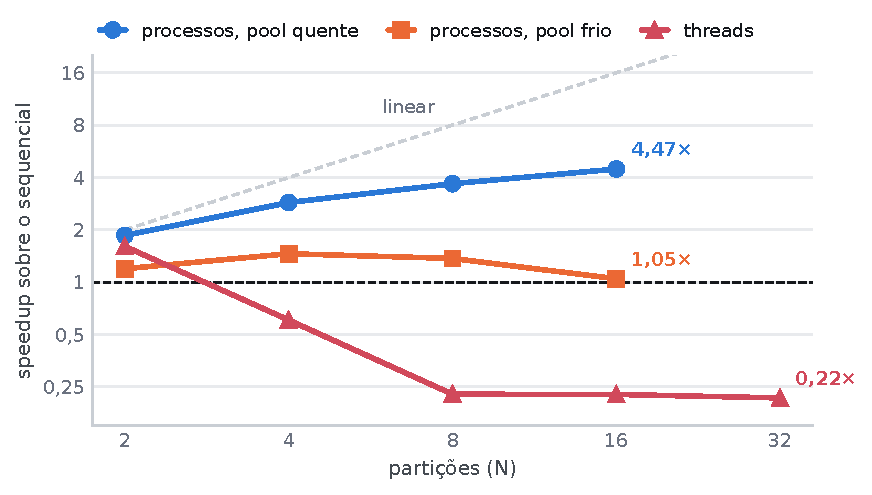
\includegraphics[width=0.85\textwidth]{assets/resultados/pool_quente.pdf}
    \captionsetup{justification=raggedright}
    \caption*{Fonte: Elaborada pelo autor}
    \label{fig:poolQuente}
\end{figure}

Três leituras se destacam. A primeira é que threads não escalam no treino: o laço de treino de uma rede pequena em CPU é dominado por código Python, que disputa o GIL, e a partir de 4 partições as threads ficam mais lentas que a execução sequencial. A segunda é que a forma de medir decide a conclusão: com o pool criado e destruído dentro da medição, como na primeira versão do experimento, cada medição inclui a inicialização de $N$ interpretadores, e o \textit{speedup} em $N = 16$ parece nulo (1,05$\times$); com o pool aquecido, o mesmo arranjo entrega 4,47$\times$. O custo de partida chega a 78\% do tempo do pool frio em $N = 16$ e foi registrado à parte, para que continue visível. A terceira é que o desenho escala, mas a máquina não acompanha: uma partição que leva 0,80 s sozinha leva 2,65 s com 16 executando juntas, 3,30 vezes mais lenta. A causa provável é a disputa de banda de memória e de \textit{cache} entre os processos, que não foi medida diretamente; outras causas, como a redução da frequência dos núcleos sob carga, não foram descartadas.

Em processos, a partição produz o mesmo resultado que a execução sequencial das mesmas partições: a OA é idêntica nas duas para $N = 2$, 4, 8 e 16. O paralelismo por processos, porém, esbarra em memória antes de esbarrar em núcleos. No experimento 13, cada processo criado por \textit{spawn} ocupa cerca de 481 MB de memória proporcional, e 32 processos exigiriam 15,4 GB em uma máquina de 15,8 GB; a configuração foi recusada antes de executar. Há também um limite de dados: com 32 partições restam cerca de 272 amostras de treino em cada uma, e a OA do modo independente cai para 0,850, contra 0,900 a 0,915 com 2 a 16 partições. Como cada partição treina e avalia um modelo próprio, com lote 64, 25 épocas e uma única semente, essas acurácias servem apenas para comparar números de partições entre si, e não são comparáveis à do modelo único. No modo replicado (experimento 11), em que um único modelo treinado com a cena inteira é usado para inferir as partições, a OA é idêntica à do modelo único (0,883), mas a inferência representa 0,4\% da execução, e não há o que ganhar.

\subsection{Fusão Concorrente}
\label{subsec:resFusao}

A fusão concorrente foi medida na inferência de todos os pixels rotulados de cada cena --- 10.249 em Indian Pines, 42.776 em University of Pavia e 54.129 em Salinas Valley ---, com o modelo da configuração herdada treinado com o treino completo. As referências são duas: o lote, que segmenta a cena e depois infere todos os pixels de uma vez, como faz o fluxo original, executado com uma e com 16 threads internas do PyTorch; e a execução sequencial por blocos, na mesma granularidade das tarefas concorrentes. O esquema foi medido nas duas formas da \autoref{subsec:fusaoConcorrente}, como no esquema e na variante desacoplada, com 1, 2, 4, 8 e 16 threads de trabalho, blocos de 1, 64 e 1.024 posições --- o bloco de uma posição apenas em Indian Pines, porque nas outras cenas seriam dezenas de milhares de tarefas por execução --- e as duas extensões da seção crítica, com 5 repetições por configuração (3 com bloco de uma posição). Em todas as 723 execuções, 660 delas da fusão concorrente, os identificadores lidos do mapa foram os mesmos usados no treino e as classes previstas foram idênticas às do lote.

O limite do esquema é dado pela segmentação: se toda a inferência fosse escondida atrás dela, o tempo de parede seria o próprio tempo do SEEDS, e o \textit{speedup} sobre o lote seria a razão entre o tempo do lote e o da segmentação. Esse teto, calculado com o tempo médio da segmentação nas execuções sequenciais por blocos, é de 2,98$\times$ em Indian Pines, onde a segmentação leva 0,111 s, mas de apenas 1,21$\times$ em University of Pavia e 1,49$\times$ em Salinas Valley, onde ela leva 0,869 s e 0,670 s e domina o tempo do lote. O \autoref{qua:fusao} e a \autoref{fig:fusaoSpeedup}, ambos com a seção crítica como no esquema, mostram o \textit{speedup} obtido sobre o lote com uma thread do PyTorch.

\begin{quadro}[!htbp]
    \centering
    \caption{\textit{Speedup} da fusão concorrente sobre o lote com uma thread do PyTorch, por número de threads de trabalho}
    \resizebox{\textwidth}{!}{%
    \begin{tabular}{|l|l|c|c|c|c|c|c|}
        \hline
        \rowcolor[HTML]{C0C0C0}
        \textbf{Cena} & \textbf{Configuração} & \textbf{N = 1} & \textbf{N = 2} & \textbf{N = 4} & \textbf{N = 8} & \textbf{N = 16} & \textbf{Teto} \\
        \hline
        Indian Pines & como no esquema, bloco 1 & 0,14$\times$ & 0,08$\times$ & 0,03$\times$ & 0,03$\times$ & 0,03$\times$ & \multirow{4}{*}{2,98$\times$} \\
                     & como no esquema, bloco 64 & 1,18$\times$ & 1,38$\times$ & 1,28$\times$ & 0,95$\times$ & 0,99$\times$ & \\
                     & como no esquema, bloco 1.024 & 1,20$\times$ & 1,64$\times$ & 0,96$\times$ & 2,01$\times$ & 1,93$\times$ & \\
                     & desacoplada, bloco 1.024 & 1,10$\times$ & 1,22$\times$ & 1,53$\times$ & 2,17$\times$ & 1,86$\times$ & \\
        \hline
        University of Pavia & como no esquema, bloco 64 & 0,82$\times$ & 0,81$\times$ & 0,71$\times$ & 0,68$\times$ & 0,63$\times$ & \multirow{3}{*}{1,21$\times$} \\
                            & como no esquema, bloco 1.024 & 1,04$\times$ & 1,19$\times$ & 1,21$\times$ & 1,11$\times$ & 1,07$\times$ & \\
                            & desacoplada, bloco 1.024 & 1,18$\times$ & 1,21$\times$ & 1,12$\times$ & 1,16$\times$ & 1,21$\times$ & \\
        \hline
        Salinas Valley & como no esquema, bloco 64 & 0,92$\times$ & 0,97$\times$ & 0,70$\times$ & 0,59$\times$ & 0,65$\times$ & \multirow{3}{*}{1,49$\times$} \\
                       & como no esquema, bloco 1.024 & 1,28$\times$ & 1,42$\times$ & 1,42$\times$ & 1,50$\times$ & 1,45$\times$ & \\
                       & desacoplada, bloco 1.024 & 1,43$\times$ & 1,54$\times$ & 1,43$\times$ & 1,57$\times$ & 1,43$\times$ & \\
        \hline
    \end{tabular}%
    }
    \captionsetup{justification=raggedright}
    \caption*{Fonte: Elaborado pelo autor. Seção crítica como no esquema; a versão mínima difere dentro da variação entre repetições. O lote leva 0,330 s, 1,050 s e 1,000 s nas três cenas. O teto usa o tempo médio da segmentação nas execuções sequenciais por blocos (0,111 s, 0,869 s e 0,670 s); como esse tempo varia entre execuções (de 0,61 s a 0,79 s nas execuções sequenciais de Salinas Valley), configurações isoladas podem ficar um pouco acima dele, como em Salinas Valley}
    \label{qua:fusao}
\end{quadro}

\begin{figure}[!htbp]
    \centering
    \captionsetup{justification=centering}
    \caption{\textit{Speedup} da fusão concorrente sobre o lote com uma thread do PyTorch, por número de threads de trabalho e granularidade}
    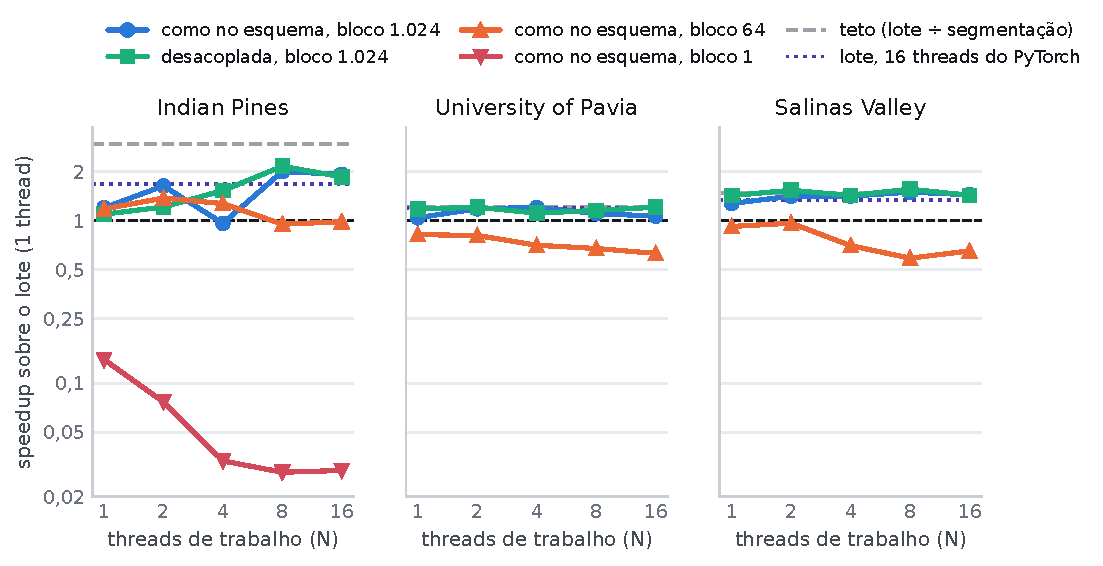
\includegraphics[width=\textwidth]{assets/resultados/fusao_speedup.pdf}
    \captionsetup{justification=raggedright}
    \caption*{Fonte: Elaborada pelo autor. Seção crítica como no esquema, a mesma do \autoref{qua:fusao}; as linhas de referência marcam o teto e o lote com 16 threads do PyTorch, e o eixo vertical está em escala logarítmica}
    \label{fig:fusaoSpeedup}
\end{figure}

Quatro leituras se destacam. A primeira é que, com a granularidade de uma posição por tarefa, o esquema fica de 7 a 35 vezes mais lento que o lote: em Indian Pines, a inferência que o lote faz em 0,33 s leva 2,35 s com uma thread de trabalho e de 9,9 s a 11,6 s com quatro ou mais. A maior parte desse custo vem de chamar a rede inteira para um único pixel, pois a execução sequencial com blocos de uma posição, sem threads, já leva 1,03 s, 3,12 vezes o tempo do lote. Com threads, a disputa pelo GIL agrava a perda, e a própria segmentação em T0, que disputa o mesmo GIL, fica duas a quatro vezes mais lenta.

A segunda é que, com blocos maiores, o esquema atinge o teto em University of Pavia e Salinas Valley. Com blocos de 1.024 posições, o tempo de parede nessas cenas fica a poucos centésimos de segundo do tempo da segmentação: toda a inferência acontece enquanto T0 segmenta ou logo depois, nas threads de trabalho, e o \textit{speedup} chega a 1,21$\times$ e 1,50$\times$, contra tetos de 1,21$\times$ e 1,49$\times$. Como o teto foi calculado com o tempo médio da segmentação, que varia entre execuções, distâncias de poucos por cento a ele, para cima ou para baixo, estão dentro dessa variação. Em Indian Pines, onde a segmentação é curta, as $N$ threads também dividem a inferência entre si, e o esquema chega a 2,01$\times$, ainda distante do teto de 2,98$\times$; a série dessa cena não é monotônica, e com 4 threads, em que a segmentação levou em média 0,27 s, mais que o dobro das demais configurações, o \textit{speedup} cai para 0,96$\times$. Com blocos de 64 posições, as 669 tarefas de University of Pavia e as 846 de Salinas Valley já tornam o esquema mais lento que o lote.

A terceira diz respeito à sobreposição. A \autoref{fig:fusaoLinhaTempo} mostra a linha do tempo de uma execução em University of Pavia, na forma como no esquema e na variante desacoplada. Na forma como no esquema, cada thread de trabalho faz as convoluções do primeiro bloco e fica bloqueada à espera do mapa; enquanto T0 segmenta, só $N$ blocos avançam. Em University of Pavia e Salinas Valley, a fração das convoluções terminadas antes da publicação do mapa vai de 0,1\%, em Salinas Valley com blocos de 64 posições e uma thread de trabalho, a 38\%, em University of Pavia com blocos de 1.024 posições e 16 threads; em Indian Pines, com 16 threads e blocos de 1.024 posições, os $N$ primeiros blocos já cobrem a cena inteira. Na variante desacoplada, em University of Pavia e Salinas Valley, todas as convoluções terminam durante a segmentação; em Indian Pines, onde a segmentação é curta, isso só ocorre com mais de uma thread de trabalho e blocos de 64 ou 1.024 posições (com uma thread, terminam em média 91\% e 94\% delas, e com blocos de uma posição, de 3\% a 13\%).

\begin{figure}[H]
    \centering
    \captionsetup{justification=centering}
    \caption{Linha do tempo de uma execução da fusão concorrente em University of Pavia, como no esquema e na variante desacoplada (4 threads de trabalho, blocos de 64 posições)}
    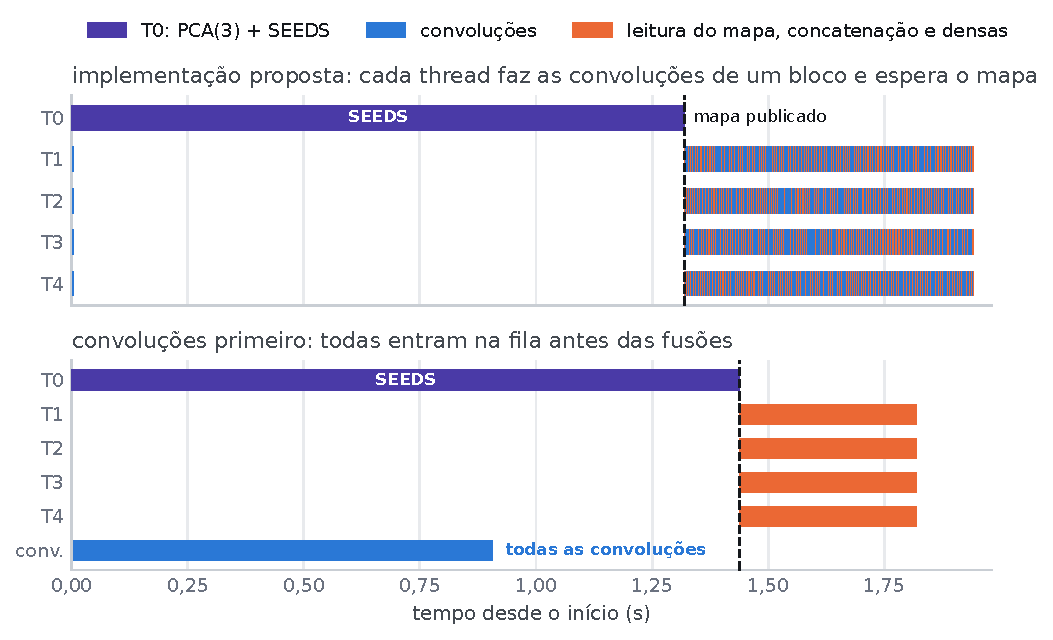
\includegraphics[width=\textwidth]{assets/resultados/fusao_linha_do_tempo.pdf}
    \captionsetup{justification=raggedright}
    \caption*{Fonte: Elaborada pelo autor. Execuções isoladas; a segmentação levou 1,10 s na forma como no esquema e 0,90 s na variante desacoplada}
    \label{fig:fusaoLinhaTempo}
\end{figure}

Na execução da figura, com blocos de 64 posições, o restante leva 0,62 s na forma como no esquema e 0,32 s na variante desacoplada depois da publicação do mapa; a diferença no tempo total (1,72 s contra 1,22 s) também reflete a segmentação, que levou 1,10 s e 0,90 s nessas duas execuções, e nas médias de 5 repetições a diferença é de 1,48 s contra 1,25 s. Com blocos de 1.024 posições, as duas formas ficam próximas em University of Pavia e Salinas Valley (\autoref{qua:fusao}), porque depois da publicação as $N$ threads concluem rapidamente o restante. Em Indian Pines, onde a segmentação é curta, o ganho vem sobretudo de dividir a inferência entre threads; em University of Pavia e Salinas Valley, a variante desacoplada com uma única thread de trabalho, que só antecipa as convoluções, já fica perto do teto (1,18$\times$ e 1,43$\times$). A extensão da seção crítica também não fez diferença mensurável: as duas versões ficaram dentro da variação entre repetições, e travar a concatenação não chegou a serializar as threads de forma visível.

A quarta leitura põe o resultado em perspectiva. Contra o lote executado com as 16 threads internas do PyTorch, que é o paralelismo dentro de cada operação já oferecido pela biblioteca, a melhor configuração com blocos de 1.024 posições rende de 1,01$\times$, em University of Pavia, a 1,29$\times$, em Indian Pines, uma economia de 0,01 s a 0,10 s por cena. Além disso, a inferência é uma parte pequena de uma execução completa, dominada pelo treino. O esquema é, portanto, uma forma correta e verificada de executar a proposta do projeto. Seu ganho aparece no cenário em que um modelo já treinado classifica uma cena nova, no qual segmentação e inferência são todo o trabalho, e fica entre 1,01$\times$ e 1,29$\times$ contra o lote com 16 threads; é limitado pelo tempo da segmentação e não tem efeito sobre o treino.

\section{Automação de Hiperparâmetros}
\label{sec:resHPO}

\subsection{Estratégias de Busca}

O \autoref{qua:estrategias} e a \autoref{fig:estrategias} comparam as três estratégias com o mesmo espaço, o mesmo número de \textit{trials} (20), a mesma cobertura inicial e três orçamentos de épocas por \textit{trial}, em Indian Pines, com 3 sementes por célula (540 \textit{trials} ao todo). A métrica de seleção é a melhor acurácia de validação; a OA de teste do vencedor é apenas relatada.

\begin{quadro}[H]
    \centering
    \caption{Estratégias de busca por orçamento de épocas (Indian Pines, 3 sementes)}
    \begin{tabular}{|p{0.16\textwidth}|p{0.14\textwidth}|c|c|}
        \hline
        \rowcolor[HTML]{C0C0C0}
        \textbf{Orçamento} & \textbf{Estratégia} & \textbf{Melhor validação} & \textbf{OA de teste do vencedor} \\
        \hline
        10 épocas & Aleatória & 0,7174 $\pm$ 0,0027 & 0,7065 \\
                  & TPE & 0,7226 $\pm$ 0,0162 & 0,7130 \\
                  & Genética & 0,7334 $\pm$ 0,0199 & 0,7174 \\
        \hline
        40 épocas & Aleatória & 0,7802 $\pm$ 0,0156 & 0,7729 \\
                  & TPE & 0,7924 $\pm$ 0,0193 & 0,7997 \\
                  & Genética & 0,8058 $\pm$ 0,0114 & 0,7989 \\
        \hline
        200 épocas & Aleatória & 0,8067 $\pm$ 0,0149 & 0,7859 \\
                   & TPE & 0,8266 $\pm$ 0,0175 & 0,8127 \\
                   & Genética & 0,8288 $\pm$ 0,0346 & 0,8080 \\
        \hline
    \end{tabular}
    \captionsetup{justification=raggedright}
    \caption*{Fonte: Elaborado pelo autor}
    \label{qua:estrategias}
\end{quadro}

\begin{figure}[H]
    \centering
    \captionsetup{justification=centering}
    \caption{Melhor acurácia de validação por estratégia e orçamento de épocas}
    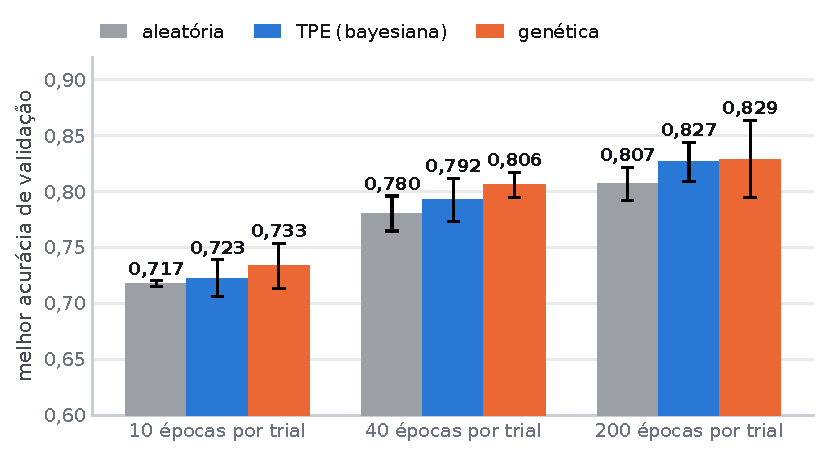
\includegraphics[width=0.85\textwidth]{assets/resultados/estrategias_hpo.pdf}
    \captionsetup{justification=raggedright}
    \caption*{Fonte: Elaborada pelo autor}
    \label{fig:estrategias}
\end{figure}

Nenhuma estratégia se separa das outras além do ruído entre sementes. As adaptativas (TPE e genética) ficam à frente da busca aleatória em todos os orçamentos, mas a diferença máxima, de 2,56 pontos com 40 épocas, é da mesma ordem do desvio médio entre sementes, de 1,3 a 2,2 pontos conforme o orçamento. Nas condições medidas (Indian Pines, 10\% do treino, 20 \textit{trials} e 3 sementes), o que mais mudou o resultado foi o orçamento: passar de 10 para 200 épocas por \textit{trial} acrescenta de 9 a 10 pontos à melhor validação, para qualquer estratégia, e a busca aleatória com 200 épocas empata com as estratégias adaptativas com 40 e supera as três com 10. Com um espaço em que poucos hiperparâmetros dominam, o sorteio já encontra a região de bons resultados, como previsto por \citeonline{Bergstra2012Random}, e o que limita a busca é quanto cada candidato pode treinar.

\subsection{Peso de Cada Hiperparâmetro}

A \autoref{fig:eixos} mostra a acurácia de validação média dos 540 \textit{trials} por valor de cada hiperparâmetro. O \textit{dropout} é o hiperparâmetro mais influente, com 18,10 pontos entre o melhor e o pior valor, seguido da taxa de aprendizado (15,26), do número de componentes do PCA (8,35), do \textit{weight decay} (4,55) e do tamanho do lote (1,81). O segmentador, que também faz parte do espaço de busca e não aparece na figura, separa 14,89 pontos nessa mesma medida, com o SEEDS à frente. A receita herdada usa o pior valor do hiperparâmetro mais influente: o \textit{dropout} de 0,5 fica 18,10 pontos abaixo do de 0,20. Nas condições medidas, com 10\% do treino em uma única cena, regularizar demais foi o erro mais caro. Essas médias, porém, misturam \textit{trials} de três orçamentos de épocas, escolhidos por estratégias diferentes, e não isolam o efeito de cada hiperparâmetro.

\begin{figure}[H]
    \centering
    \captionsetup{justification=centering}
    \caption{Acurácia de validação média por valor de cada hiperparâmetro do espaço de busca, com o valor herdado destacado}
    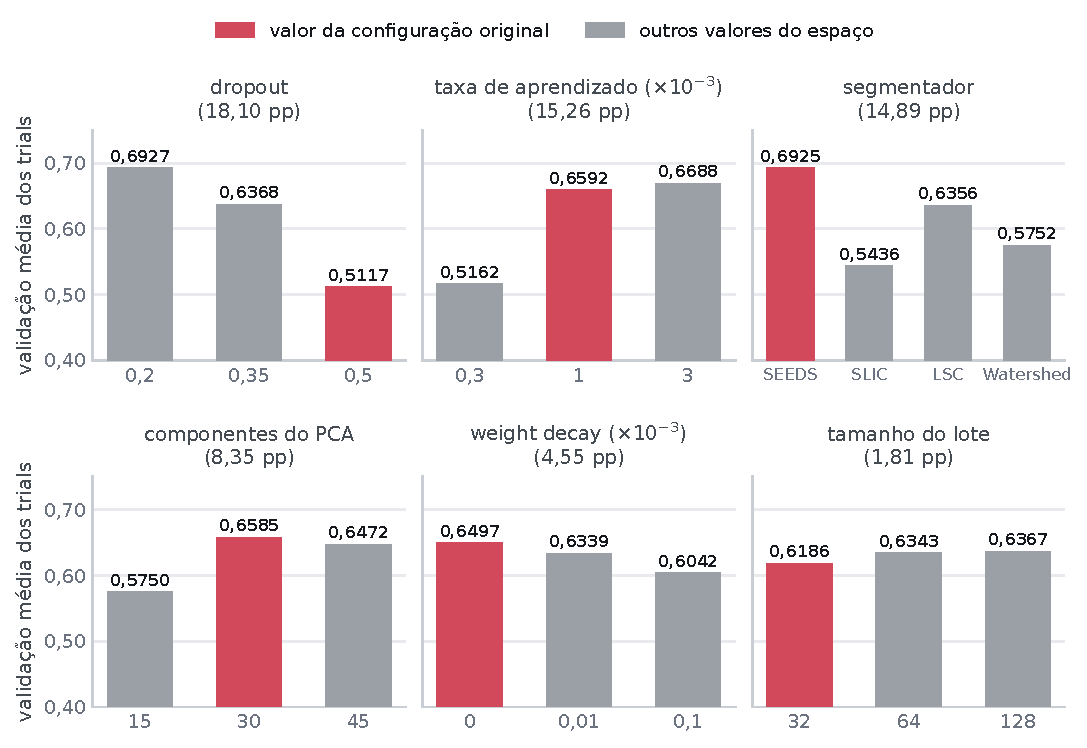
\includegraphics[width=\textwidth]{assets/resultados/eixos_hpo.pdf}
    \captionsetup{justification=raggedright}
    \caption*{Fonte: Elaborada pelo autor. Taxa de aprendizado e \textit{weight decay} em unidades de $10^{-3}$; entre parênteses, a diferença entre o melhor e o pior valor de cada hiperparâmetro, em pontos percentuais}
    \label{fig:eixos}
\end{figure}

\subsection{Ganho sobre a Receita Herdada}

O \autoref{qua:impactoHPO} e a \autoref{fig:impactoHPO} respondem à pergunta central deste eixo: quanto se ganha ao substituir a receita herdada pela receita encontrada pela busca. Para cada segmentador, as duas receitas foram treinadas com as mesmas 5 sementes, em Indian Pines, com 10\% do treino. A receita herdada é a do notebook original --- taxa de aprendizado 0,001, \textit{dropout} 0,5, \textit{weight decay} 0, lote 32 e 30 componentes ---, e a otimizada é a vencedora da busca TPE do mesmo segmentador (\autoref{ap:receitas}); as duas são treinadas com a regra de parada da \autoref{subsec:desTreino}. Um ganho é considerado afirmável quando excede duas vezes o desvio combinado das duas receitas entre sementes.

\begin{quadro}[H]
    \centering
    \caption{Receita herdada contra receita otimizada (Indian Pines, 5 sementes, 10\% do treino)}
    \resizebox{\textwidth}{!}{%
    \begin{tabular}{|l|c|c|c|c|l|}
        \hline
        \rowcolor[HTML]{C0C0C0}
        \textbf{Segmentador} & \textbf{OA herdada} & \textbf{OA otimizada} & \textbf{Ganho (pp)} & \textbf{Desvio comb.} & \textbf{Leitura} \\
        \hline
        SEEDS (herdado) & 0,7441 $\pm$ 0,0169 & 0,8174 $\pm$ 0,0112 & +7,33 & 2,03 & afirmável \\
        \hline
        SLIC & 0,6060 $\pm$ 0,1603 & 0,6411 $\pm$ 0,1856 & +3,51 & 24,53 & ruído \\
        \hline
        LSC & 0,6814 $\pm$ 0,0381 & 0,7566 $\pm$ 0,0219 & +7,52 & 4,39 & ruído \\
        \hline
        Watershed & 0,5847 $\pm$ 0,1586 & 0,5646 $\pm$ 0,2255 & $-$2,00 & 27,57 & ruído \\
        \hline
    \end{tabular}%
    }
    \captionsetup{justification=raggedright}
    \caption*{Fonte: Elaborado pelo autor}
    \label{qua:impactoHPO}
\end{quadro}

\begin{figure}[H]
    \centering
    \captionsetup{justification=centering}
    \caption{OA de teste com a receita herdada (lote 32) e com a receita otimizada, por segmentador (Indian Pines, 5 sementes, 10\% do treino)}
    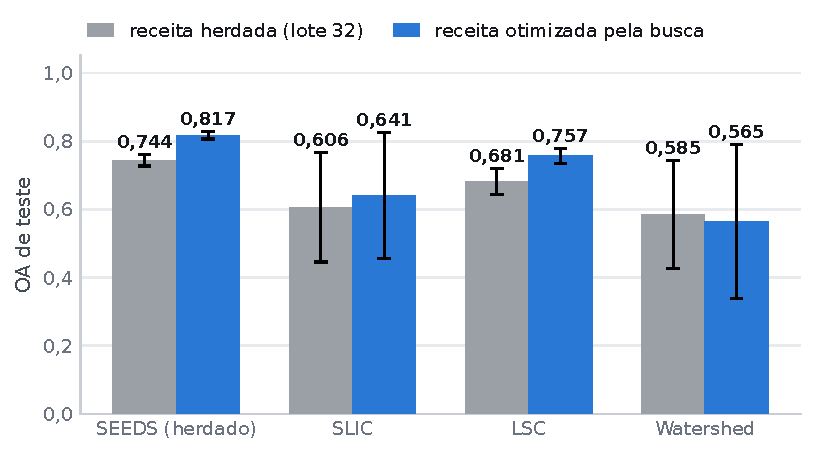
\includegraphics[width=0.85\textwidth]{assets/resultados/impacto_hpo.pdf}
    \captionsetup{justification=raggedright}
    \caption*{Fonte: Elaborada pelo autor. As barras de erro indicam o desvio padrão entre sementes}
    \label{fig:impactoHPO}
\end{figure}

Na configuração do trabalho de referência, com o SEEDS, a busca acrescenta 7,33 pontos de OA, 10,81 de AA e 8,52 de Kappa, e esse é o único ganho deste eixo que se separa do ruído entre sementes; na AA, por margem mínima, já que o limiar, de duas vezes o desvio combinado, é de 10,78 pontos. A receita vencedora reduz o \textit{dropout} de 0,5 para 0,35, dobra o tamanho do lote e usa 15 componentes do PCA em vez de 30, mantendo a taxa de aprendizado herdada. A redução do \textit{dropout} é coerente com o peso dos hiperparâmetros medido acima, em que o valor herdado é o pior do hiperparâmetro mais influente, enquanto a escolha de 15 componentes não é, pois esse é o pior valor médio do número de componentes do PCA; como as três mudanças vieram juntas, o efeito de cada uma não foi isolado. Para os demais segmentadores, o desvio entre sementes é grande demais para afirmar o sinal do ganho: SLIC e Watershed colapsam em algumas sementes com qualquer das duas receitas, e o ganho do LSC, de 7,52 pontos, fica abaixo do limiar de 8,78. Esse ganho foi medido com 10\% do treino, que é o regime em que a busca foi feita. Com o treino completo, apenas a configuração herdada foi medida, e seus valores absolutos são os do \autoref{qua:linhaBase}; o efeito da receita otimizada nesse regime não foi medido.

\section{Segmentadores}
\label{sec:resSegmentadores}

\subsection{O que Cada Algoritmo Produz}

O \autoref{qua:estruturaSeg} resume a estrutura das segmentações com os parâmetros padrão. O SEEDS produz poucas regiões grandes (81 em Indian Pines e 45 em University of Pavia), enquanto SLIC e LSC produzem quatro vezes mais regiões em Indian Pines e cerca de trinta vezes mais em University of Pavia. A pureza, isto é, a fração da classe dominante dentro de cada região, é maior no LSC e no SLIC. Todos os algoritmos são rápidos em relação ao treino; o SEEDS é o mais lento nas duas cenas, e o Watershed, o mais rápido.

\begin{quadro}[H]
    \centering
    \caption{Estrutura das segmentações com os parâmetros padrão}
    \begin{tabular}{|l|l|c|c|c|c|}
        \hline
        \rowcolor[HTML]{C0C0C0}
        \textbf{Cena} & \textbf{Algoritmo} & \textbf{Regiões} & \textbf{Área média (px)} & \textbf{Pureza} & \textbf{Tempo (s)} \\
        \hline
        Indian Pines & SEEDS & 81 & 259,6 & 0,8831 & 0,149 \\
                     & SLIC & 324 & 64,9 & 0,9581 & 0,051 \\
                     & LSC* & 324 & 64,9 & 0,9699 & 0,031 \\
                     & Watershed & 273 & 77,0 & 0,8543 & 0,004 \\
        \hline
        University of Pavia & SEEDS & 45 & 4.608,9 & 0,9212 & 1,854 \\
                    & SLIC & 1.428 & 145,2 & 0,9857 & 0,263 \\
                    & LSC* & 1.428 & 145,2 & 0,9955 & 0,203 \\
                    & Watershed & 421 & 492,6 & 0,9313 & 0,030 \\
        \hline
    \end{tabular}
    \captionsetup{justification=raggedright}
    \caption*{Fonte: Elaborado pelo autor. * LSC medido antes da correção do seu não determinismo. Tempos de uma medição avulsa dos segmentadores isolados, em sessão distinta; não são comparáveis aos do \autoref{qua:ramos} nem aos da \autoref{subsec:resFusao}, em que o SEEDS leva cerca de 0,11 s em Indian Pines e 0,87 s em University of Pavia}
    \label{qua:estruturaSeg}
\end{quadro}

\subsection{A Comparação com a CNN Fixa}

A primeira comparação, prevista no plano de verificação, manteve os hiperparâmetros da CNN fixos para os quatro segmentadores. Em University of Pavia, o SEEDS obteve Kappa de 0,9360, enquanto o SLIC obteve 0,0346, praticamente o de um classificador aleatório, e o LSC, 0,1970 com desvio de 0,35 entre sementes (medido antes da correção do seu não determinismo). A explicação está na escala da segunda entrada: com 1.428 regiões, o identificador concatenado vai até 1.428, contra componentes espectrais de variância unitária, e a receita que serve ao SEEDS, com 45 regiões, não serve a esses algoritmos. Algumas sementes treinam e outras colapsam, o que explica o desvio. A conclusão que esse desenho sugeriria, de que o SLIC não serve para University of Pavia, é desmentida pela otimização conjunta a seguir, e o desenho foi mantido apenas como contraexemplo.

\subsection{Sob Otimização Conjunta}

O \autoref{qua:segmentadores} e a \autoref{fig:segmentadores} mostram a OA de cada segmentador quando a CNN é otimizada para ele, com o mesmo orçamento de busca, nas três cenas. As receitas vencedoras estão no \autoref{ap:receitas}.

\begin{quadro}[H]
    \centering
    \caption{OA de teste de cada segmentador sob otimização conjunta (5 sementes, 10\% do treino)}
    \resizebox{\textwidth}{!}{%
    \begin{tabular}{|l|c|c|c|c|}
        \hline
        \rowcolor[HTML]{C0C0C0}
        \textbf{Cena} & \textbf{SEEDS (herdado)} & \textbf{SLIC} & \textbf{LSC*} & \textbf{Watershed} \\
        \hline
        Indian Pines & 0,8174 $\pm$ 0,0112 & 0,6411 $\pm$ 0,1856 & 0,7446 $\pm$ 0,0284 & 0,5646 $\pm$ 0,2255 \\
        \hline
        University of Pavia & 0,9515 $\pm$ 0,0042 & 0,9534 $\pm$ 0,0039 & 0,9373 $\pm$ 0,0053 & 0,9555 $\pm$ 0,0020 \\
        \hline
        Salinas Valley & 0,9632 $\pm$ 0,0076 & 0,9501 $\pm$ 0,0045 & 0,9470 $\pm$ 0,0019 & 0,9497 $\pm$ 0,0046 \\
        \hline
    \end{tabular}%
    }
    \captionsetup{justification=raggedright}
    \caption*{Fonte: Elaborado pelo autor. * LSC medido antes da correção do seu não determinismo; após a correção, em Indian Pines, a mesma receita obteve 0,7566 $\pm$ 0,0219}
    \label{qua:segmentadores}
\end{quadro}

\begin{figure}[H]
    \centering
    \captionsetup{justification=centering}
    \caption{OA de teste de cada segmentador sob otimização conjunta, por cena}
    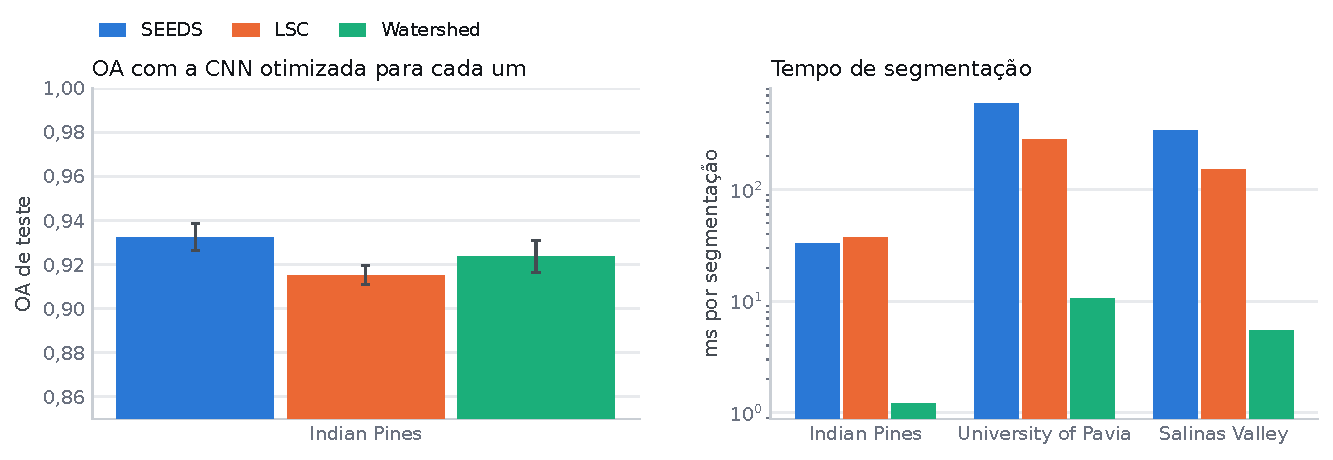
\includegraphics[width=\textwidth]{assets/resultados/segmentadores.pdf}
    \captionsetup{justification=raggedright}
    \caption*{Fonte: Elaborada pelo autor. WS: Watershed. * LSC medido antes da correção do seu não determinismo. A linha tracejada marca a OA do SEEDS, e as barras de erro, o desvio padrão entre sementes. Nos painéis de University of Pavia e Salinas Valley, o eixo vertical começa em 0,90}
    \label{fig:segmentadores}
\end{figure}

Desses resultados decorrem três conclusões. A primeira é que o segmentador é uma das escolhas de maior impacto do fluxo, embora com resultados instáveis. Em Indian Pines, 25,3 pontos de OA de teste separam o melhor do pior segmentador, cada um com a CNN otimizada para si; essa diferença, entre o SEEDS e o Watershed, vem sobretudo de duas sementes em que o Watershed colapsa e fica dentro do desvio, e a diferença afirmável nessa cena é a do SEEDS sobre o LSC, de 6,1 pontos com a receita refeita após a correção. Na análise por hiperparâmetro, que usa outra medida (a validação média por valor), o segmentador separa 14,89 pontos, atrás do \textit{dropout} (18,10) e da taxa de aprendizado (15,26).

A segunda é que nenhum segmentador supera o SEEDS herdado de forma afirmável. Em Indian Pines, todos ficam atrás mesmo otimizados para si, SLIC e Watershed com desvio muito alto; em University of Pavia, SLIC e Watershed têm média maior que a do SEEDS (+0,19 e +0,41 ponto), dentro do desvio; em Salinas Valley, SLIC e Watershed ficam 1,3 ponto atrás, também dentro do desvio, e só o LSC (1,6 ponto atrás) passa do critério, por margem mínima. Em University of Pavia e Salinas Valley, a meta de validação de 0,95 interrompe cedo parte dos treinos (em média, 2,8 épocas no SEEDS em Salinas Valley; \autoref{ap:receitas}), e diferenças dessa ordem devem ser lidas com essa ressalva.

A terceira é que cada segmentador escolhe hiperparâmetros diferentes: em Indian Pines, o SLIC foi o único a escolher uma taxa de aprendizado três vezes menor e lotes de 128, o que é coerente com a necessidade de acomodar um identificador de escala maior, que, com as regiões de 5 px da receita vencedora, vai até cerca de 840. O segmentador reconfigura o treino, e por isso não pode ser comparado com a CNN fixa.

\subsection{O que Explica o Desempenho}

A pureza das regiões não acompanha o resultado: em Indian Pines, o LSC tem a maior pureza (0,97, medida antes da correção do seu não determinismo) e fica 6,1 pontos atrás do SEEDS com a receita refeita após a correção (7,3 pontos na medição anterior), enquanto a pureza do SEEDS, de 0,88, só supera a do Watershed. O resultado é compatível com o número de amostras de treino por região: com os parâmetros padrão e 10\% do treino, são 10,8 no SEEDS, contra 2,7 no SLIC e no LSC e 3,2 no Watershed, e as receitas vencedoras do SLIC e do LSC, com regiões de 5 px, ficam perto de uma amostra por região (\autoref{qua:receitasVencedoras}). Com o treino fixo, porém, esse indicador é apenas o inverso do número de regiões, que também fixa a magnitude do identificador; ele não ordena os outros três algoritmos (o Watershed, com 3,2 amostras por região, tem a menor OA), e quatro algoritmos em uma única cena não permitem separar os dois efeitos nem afirmar uma causa.

O \autoref{qua:ablacao} ajuda a entender como o identificador é aproveitado. Cada linha altera uma propriedade do identificador do SEEDS, em Indian Pines, com 3 sementes. Substituí-lo por um número aleatório por pixel, que preserva apenas a escala, é a pior alteração, o que indica que a rede usa a informação de agrupamento. Normalizá-lo para o intervalo $[0, 1]$, que preserva tudo menos a magnitude, custa 7,58 pontos, o que indica que a rede se apoia na escala exagerada do identificador. Por fim, uma tabela de vetores aprendidos por região, que elimina tanto a ordem artificial entre identificadores quanto a dependência da escala, elevou a OA de 0,8981 para 0,9471 em Indian Pines e, na mesma comparação de modos de fusão, também com 3 sementes e fora do quadro, de 0,9785 para 0,9868 em University of Pavia. Sem o desvio registrado, essas diferenças não podem ser submetidas ao critério de afirmabilidade usado no restante do capítulo; elas sugerem, como melhoria da fusão herdada, trocar a concatenação do identificador por um vetor aprendido por região.

\begin{quadro}[H]
    \centering
    \caption{Como o identificador do superpixel é aproveitado pela rede (Indian Pines, 3 sementes)}
    \begin{tabular}{|p{0.32\textwidth}|p{0.40\textwidth}|c|}
        \hline
        \rowcolor[HTML]{C0C0C0}
        \textbf{Identificador} & \textbf{O que preserva} & \textbf{OA} \\
        \hline
        Original (herdado) & tudo & 0,8981 \\
        \hline
        Permutado entre regiões & agrupamento e escala; perde a ordem & 0,8552 \\
        \hline
        Normalizado para $[0, 1]$ & tudo menos a magnitude & 0,8223 \\
        \hline
        Aleatório por pixel & só a escala; perde o agrupamento & 0,7898 \\
        \hline
        Vetor aprendido por região & agrupamento, sem ordem nem escala & 0,9471 \\
        \hline
    \end{tabular}
    \captionsetup{justification=raggedright}
    \caption*{Fonte: Elaborado pelo autor. Médias de 3 sementes, sem o desvio registrado; a linha do vetor aprendido vem da comparação de modos de fusão, com a mesma referência. A referência (0,8981) vem de uma rodada própria e difere das médias do \autoref{qua:fracaoTreino} (0,9016) e do \autoref{qua:linhaBase} (0,9051, semente 42); as diferenças entre linhas devem ser lidas dentro deste quadro}
    \label{qua:ablacao}
\end{quadro}

\section{Verificação dos Requisitos}
\label{sec:resVerificacao}

A verificação segue o plano do \autoref{cap:proj}. O \autoref{qua:verifRF} e o \autoref{qua:verifRNF} resumem, para cada requisito, a situação e a evidência que a sustenta.

\begin{quadro}[H]
    \centering
    \caption{Verificação dos requisitos funcionais}
    \begin{tabular}{|p{0.08\textwidth}|p{0.13\textwidth}|p{0.69\textwidth}|}
        \hline
        \rowcolor[HTML]{C0C0C0}
        \textbf{Req.} & \textbf{Situação} & \textbf{Evidência} \\
        \hline
        \textbf{RF01} & Atendido & CNN 1D implementada conforme o \autoref{qua:camadas}; OA de 0,9051 a 0,9938 na configuração herdada (\autoref{qua:linhaBase}) \\
        \hline
        \textbf{RF02} & Atendido & SEEDS, SLIC, LSC e Watershed, com o mesmo formato de saída (\autoref{subsec:desSegmentadores}) e comparados no \autoref{qua:segmentadores} \\
        \hline
        \textbf{RF03} & Atendido & Concatenação do identificador do superpixel após o achatamento, com entrada de 1.025 posições na cabeça densa em Indian Pines; substituir o identificador por ruído com a mesma escala reduz a OA em 10,83 pontos, na média de 3 sementes, sem desvio registrado (\autoref{qua:ablacao}); a vantagem sobre a rede puramente espectral é a reportada por \citeonline{Souza2023} \\
        \hline
        \textbf{RF04} & Atendido & Busca aleatória, TPE e algoritmo genético (\autoref{sec:desHPO}); ganho de 7,33 pontos de OA sobre a receita herdada, em Indian Pines e com 10\% do treino (\autoref{qua:impactoHPO}) \\
        \hline
        \textbf{RF05} & Atendido em parte & OA, AA e Kappa; tempo de cada etapa e da inferência; número de parâmetros; memória retida por \textit{trial} e por processo; \textit{speedup} e seu teto teórico. O pico de memória durante o treino e a inferência, previsto no plano, não foi medido \\
        \hline
        \textbf{RF06} & Atendido & Entre os ramos (até 1,22$\times$), na fusão concorrente (até 2,01$\times$ contra o lote com uma thread do PyTorch, no teto em University of Pavia e Salinas Valley, e de 1,01$\times$ a 1,29$\times$ contra o lote com 16 threads) e por partição da cena (até 4,47$\times$) \\
        \hline
    \end{tabular}
    \captionsetup{justification=raggedright}
    \caption*{Fonte: Elaborado pelo autor}
    \label{qua:verifRF}
\end{quadro}

\begin{quadro}[H]
    \centering
    \caption{Verificação dos requisitos não funcionais}
    \begin{tabular}{|p{0.08\textwidth}|p{0.13\textwidth}|p{0.69\textwidth}|}
        \hline
        \rowcolor[HTML]{C0C0C0}
        \textbf{Req.} & \textbf{Situação} & \textbf{Evidência} \\
        \hline
        \textbf{RNF01} & Atendido & A mesma arquitetura do notebook original de \citeonline{Souza2023}, com os mesmos 37.577 parâmetros em University of Pavia \\
        \hline
        \textbf{RNF02} & Atendido & Toda a implementação em Python \\
        \hline
        \textbf{RNF03} & Atendido em parte & Treino com aceleração por GPU, em uma GPU local, e não no Google Colab ou em ambiente HPC \\
        \hline
        \textbf{RNF04} & Atendido & Fusão por concatenação do identificador ao vetor de características espectrais \\
        \hline
        \textbf{RNF05} & Atendido em parte & Com o SEEDS, em Indian Pines e com 10\% do treino, +7,33 pontos de OA, +10,81 de AA e +8,52 de Kappa sobre a receita herdada; nos demais segmentadores, o ganho fica dentro do ruído entre sementes \\
        \hline
        \textbf{RNF06} & Atendido em parte & Execuções repetidas com a mesma configuração produzem resultados idênticos; entre sementes, com o SEEDS, o desvio da OA fica entre 0,42 e 1,69 ponto, abaixo de 2, mas o da AA chega a 4,43 pontos em Indian Pines, e SLIC e Watershed em Indian Pines chegam a 22,55 pontos de OA \\
        \hline
        \textbf{RNF07} & Atendido & Redução de tempo medida nas três estratégias de paralelismo, contra a execução sequencial ou em lote no mesmo dispositivo (\autoref{sec:resParalelismo}) \\
        \hline
    \end{tabular}
    \captionsetup{justification=raggedright}
    \caption*{Fonte: Elaborado pelo autor}
    \label{qua:verifRNF}
\end{quadro}

O plano também fixou metas de acurácia por conjunto de dados (\autoref{tab:validacaoDatasets}), comparadas no \autoref{qua:metas} com a configuração herdada reimplementada, com o treino completo. A meta é atingida em Salinas Valley e não é atingida, nesta execução de semente única, em University of Pavia, por 0,28 ponto de OA, 0,56 de AA e 0,02 de Kappa, nem em Indian Pines, onde a distância é maior. A meta de Indian Pines, de 0,95 de OA, está acima do próprio valor reportado no trabalho de referência (0,9142), e o ganho de 7,33 pontos obtido pela busca de hiperparâmetros foi medido com 10\% do treino; o efeito da receita otimizada com o treino completo, que poderia aproximar Indian Pines da meta, não foi medido.

\begin{quadro}[H]
    \centering
    \caption{Metas de acurácia do projeto e valores obtidos com a configuração herdada (OA; AA; Kappa)}
    \begin{tabular}{|p{0.22\textwidth}|p{0.22\textwidth}|p{0.28\textwidth}|p{0.16\textwidth}|}
        \hline
        \rowcolor[HTML]{C0C0C0}
        \textbf{Cena} & \textbf{Meta} & \textbf{Obtido} & \textbf{Situação} \\
        \hline
        Indian Pines & 0,95; 0,93; 0,94 & 0,9051; 0,8237; 0,8914 & Não atingida \\
        \hline
        University of Pavia & 0,98; 0,97; 0,97 & 0,9772; 0,9644; 0,9698 & Não atingida \\
        \hline
        Salinas Valley & 0,97; 0,96; 0,96 & 0,9938; 0,9956; 0,9931 & Atingida \\
        \hline
    \end{tabular}
    \captionsetup{justification=raggedright}
    \caption*{Fonte: Elaborado pelo autor}
    \label{qua:metas}
\end{quadro}

\section{Discussão dos Resultados}
\label{sec:resDiscussao}

Nos eixos de desempenho, os resultados convergem para uma mesma observação: o ganho de cada otimização é limitado pela fração do trabalho que ela alcança e depende da referência contra a qual é medido. Nos eixos de acurácia, o que decidiu quais diferenças podem ser afirmadas foi o ruído entre sementes.

No paralelismo, a partição em processos e a fusão concorrente produzem os mesmos resultados que a execução sequencial e o lote, respectivamente, enquanto o treino de partições em threads não os repete, porque as threads compartilham o gerador aleatório (\autoref{sec:resOrganizacao}). O ganho de cada estratégia, porém, é limitado pela fração do tempo que ela alcança. O paralelismo entre os ramos do pré-processamento só atingiu o teto do próprio desenho em Salinas Valley, e esse teto é baixo porque a segmentação domina o pré-processamento, que por sua vez é menos de 1\% de uma execução. A fusão concorrente proposta pelo orientador atingiu, com blocos de 1.024 posições, o teto dado pela segmentação em University of Pavia e Salinas Valley, mas atua sobre a inferência, que também é uma parte pequena do total. O ganho expressivo, de até 4,47$\times$, veio de paralelizar o treino entre partições da cena com processos, em Indian Pines, com 16 partições e pool aquecido. Em todos os níveis, threads de Python só aceleraram o que acontece fora do interpretador: a segmentação e as operações do PyTorch sobre blocos grandes, e não o laço de treino nem chamadas pixel a pixel.

A forma de medir decidiu mais de uma conclusão deste eixo. Com o pool de processos criado dentro da medição, a partição parecia não ganhar nada com 16 partições; com o pool aquecido, entregou 4,47$\times$. Na primeira rodada da fusão concorrente, as operações do PyTorch em cada thread de trabalho usavam as 32 threads padrão do OpenMP, porque a restrição a uma thread, feita na thread principal, não se propaga às demais (\autoref{subsec:fusaoConcorrente}); em University of Pavia, com blocos de 64 posições e uma thread de trabalho, o esquema levava 7,3 s nessa rodada, descartada, contra 1,28 s depois da correção (\autoref{qua:fusao}). Nos dois casos, a correção veio de conferir a medição antes de interpretá-la.

Na automação de hiperparâmetros, o ganho de 7,33 pontos de OA sobre a receita herdada, medido em Indian Pines com 10\% do treino, é o resultado mais direto do trabalho em acurácia. Ele vem de uma receita que reduz o \textit{dropout}, dobra o lote e usa 15 componentes do PCA; o efeito de cada mudança não foi isolado, mas a redução do \textit{dropout} é coerente com o peso dos hiperparâmetros, em que o valor herdado é o pior do hiperparâmetro mais influente. A escolha da estratégia de busca, por outro lado, não fez diferença afirmável. Nas condições medidas, com uma cena, 10\% do treino, 20 \textit{trials} e 3 sementes, aumentar o orçamento de épocas por \textit{trial} pesou mais que trocar a estratégia: a busca aleatória com 200 épocas empatou com as estratégias adaptativas com 40 e superou as três com 10.

Nos segmentadores, a comparação com a CNN fixa, prevista no plano, levaria à conclusão falsa de que o SLIC não serve para University of Pavia; com a CNN otimizada para ele, o SLIC empata com o SEEDS nessa cena, e cada segmentador escolhe hiperparâmetros próprios. Mesmo com a CNN otimizada para cada um, nenhum dos três superou o SEEDS herdado de forma afirmável, e o resultado acompanha o número de amostras de treino por região mais do que a pureza das regiões, sem que os dados permitam afirmar uma causa.

A organização do código, por fim, é o que torna os demais resultados atribuíveis. Dois dos três defeitos descritos na \autoref{sec:resOrganizacao}, o não determinismo do LSC e o gerador aleatório compartilhado entre threads, só foram encontrados porque cada execução é reprodutível e cada experimento confere a repetibilidade das próprias medições; o terceiro, o piso de componentes do PCA, apareceu quando a campanha foi interrompida por um erro. Em relação ao trabalho de referência, a configuração herdada reimplementada fica abaixo dos valores reportados por \citeonline{Souza2023} --- por menos de 1 ponto de OA em Indian Pines e Salinas Valley, 1,6 ponto em University of Pavia e 7,2 pontos de AA em Indian Pines ---, o que é coerente com uma política de parada única para as três cenas, em vez de ajustes por conjunto de dados, e com uma única execução de cada lado.
 \clearpage
\chapter{Considerações Finais}
\label{cap:consid}

Este trabalho partiu da arquitetura de \citeonline{Souza2023}, uma CNN 1D com a fusão do identificador do superpixel SEEDS, e a otimizou em quatro eixos (organização do código, paralelismo, automação de hiperparâmetros e segmentadores), medindo cada ganho contra a configuração original, com a fusão. A rede foi reimplementada em PyTorch, em um pacote modular e determinístico, e sobre essa base foram implementadas três estratégias de paralelismo, três estratégias de busca de hiperparâmetros e quatro algoritmos de segmentação, avaliados em Indian Pines, University of Pavia e Salinas Valley.

\section{Objetivos}

O primeiro objetivo, reimplementar a arquitetura de forma modular e reprodutível, foi atendido: a reimplementação preserva a arquitetura, o PCA, a divisão dos dados e os hiperparâmetros de treino, troca a regra de parada antecipada (\autoref{subsec:desTreino}) e produz sempre o mesmo resultado para a mesma configuração. Os valores reportados por \citeonline{Souza2023} ficam acima dos da reimplementação por menos de 1 ponto de OA em Indian Pines e Salinas Valley, 1,6 ponto em University of Pavia e 7,2 pontos de AA em Indian Pines, em uma execução de cada lado (\autoref{tab:linhaBase}). A organização também revelou três defeitos (\autoref{sec:resOrganizacao}): o não determinismo do LSC, o gerador aleatório compartilhado entre threads e o piso de componentes do PCA.

O segundo, explorar algoritmos de segmentação, foi atendido com SEEDS, SLIC, LSC e Watershed sob otimização conjunta (\autoref{sec:resSegmentadores}). O segmentador é uma das escolhas de maior impacto: na validação média dos 540 \textit{trials}, separa 14,89 pontos, atrás apenas do \textit{dropout} e da taxa de aprendizado (\autoref{fig:eixos}). Nenhum segmentador superou o SEEDS de forma afirmável, e a pureza das regiões não acompanhou o resultado (\autoref{tab:estruturaSeg}); o número de amostras de treino por região é maior no SEEDS, o de melhor resultado, mas não ordena os outros três, e quatro segmentadores de uma única cena não demonstram uma causa.

O terceiro, o ajuste automático de hiperparâmetros, foi atendido com busca aleatória, TPE e algoritmo genético, que substituíram a busca em grade e a Otimização Bayesiana com processo gaussiano previstas no projeto (\autoref{sec:desHPO}, \autoref{sec:resHPO}). Com o SEEDS, a busca elevou a OA de Indian Pines de 0,7441 para 0,8174, com 10\% do treino e 5 sementes, um ganho de 7,33 pontos de OA, 10,81 de AA e 8,52 de Kappa (\autoref{tab:impactoHPO} e \autoref{tab:impactoHPOCompleto}); o ganho com o treino completo não foi medido, e o efeito de cada mudança da configuração vencedora não foi isolado. Nenhuma estratégia se separou do ruído entre sementes (\autoref{tab:estrategias}), e o orçamento de épocas por \textit{trial} pesou mais que a estratégia.

O quarto, o processamento paralelo, foi atendido em três níveis (\autoref{sec:resParalelismo}). Entre os ramos do pré-processamento, o ganho chegou a 1,22$\times$, no teto do desenho, apenas em Salinas Valley (\autoref{tab:ramos}), e o pré-processamento é 0,9\% da execução. A partição da cena com processos e pool aquecido acelerou o treino em até 4,47$\times$ com 16 partições em Indian Pines (\autoref{tab:poolQuente}), enquanto as threads, limitadas pelo GIL, ficaram mais lentas que a execução sequencial a partir de 4 partições. A fusão concorrente, implementada com uma variável de condição e validada em 723 execuções com as mesmas classes do lote, atingiu o teto dado pela segmentação em University of Pavia e Salinas Valley e chegou a 2,01$\times$ em Indian Pines contra o lote com uma thread do PyTorch (\autoref{tab:fusao}); contra o lote com 16 threads, rende de 1,01$\times$ a 1,29$\times$, e com uma posição por tarefa fica de 7 a 35 vezes mais lenta.

O quinto, a análise comparativa por métricas de acurácia e custo computacional, corresponde ao \autoref{cap:resultados}, que reporta OA, AA, Kappa, tempo, memória e \textit{speedup} contra referências explícitas. Com os objetivos específicos cumpridos, foi atendido o objetivo geral de analisar o impacto de técnicas de segmentação, parametrização automática e processamento paralelo na classificação de imagens hiperespectrais com CNNs 1D.

\section{Hipóteses}

\begin{enumerate}
    \item \textit{Diferentes algoritmos de segmentação apresentarão desempenhos variados em termos de acurácia e tempo de processamento, sendo possível identificar alternativas ao SEEDS para cenários específicos.} Confirmada em parte: os desempenhos variam, mas nenhuma alternativa superou o SEEDS em acurácia de forma afirmável. Em University of Pavia, o Watershed segmentou cerca de 60 vezes mais rápido que o SEEDS (\autoref{tab:estruturaSeg}), o que o torna candidato quando a segmentação pesa no tempo total, como na inferência de uma cena nova.
    \item \textit{A otimização automática de hiperparâmetros identificará configurações superiores ao ajuste manual, melhorando métricas de acurácia (OA, AA, Kappa) de forma reprodutível.} Confirmada para a configuração de referência, com o SEEDS em Indian Pines e 10\% do treino; para os demais segmentadores, o ganho de OA ficou dentro do ruído entre sementes (\autoref{tab:impactoHPO}).
    \item \textit{A otimização conjunta de segmentação e CNN superará a otimização isolada de cada componente.} Não testada como formulada, porque a otimização isolada de cada componente não foi executada. Os resultados mostram que a comparação com a CNN fixa é inválida: com a configuração do SEEDS, o SLIC obteve Kappa de 0,03 em University of Pavia e, otimizado para si, empatou com o SEEDS.
    \item \textit{A paralelização do processamento espacial e espectral resultará em redução mensurável do tempo de execução em relação à implementação sequencial, explorando a independência de dados entre as operações e a execução concorrente via threads.} Confirmada com ressalvas: as duas estratégias com threads reduziram o tempo (até 1,22$\times$ e 2,01$\times$), mas sobre etapas pequenas de uma execução dominada pelo treino; a maior redução, de 4,47$\times$, veio da partição com processos.
\end{enumerate}

\section{Limitações}

A busca de hiperparâmetros e a comparação de segmentadores usaram 10\% do treino, e o ganho da busca com o treino completo não foi medido. A comparação de estratégias, o ganho sobre a configuração original, a partição da cena e a fusão concorrente com uma posição por tarefa foram medidos apenas em Indian Pines. A linha de base compara uma execução de cada lado, e a ablação do identificador usa 3 sementes, sem desvio registrado. As medições de tempo foram feitas em uma única máquina, cujo número de núcleos e memória condicionam os \textit{speedups}.

\section{Trabalhos Futuros}

\begin{itemize}
    \item \textbf{Fusão por vetores aprendidos}: substituir o identificador numérico por um vetor aprendido por região, que elevou a OA de 0,8981 para 0,9471 em Indian Pines (\autoref{tab:ablacao}), e avaliá-lo com mais sementes e com os quatro segmentadores;
    \item \textbf{Paralelismo sem GIL}: repetir a fusão concorrente e a partição em threads em uma versão do CPython sem a trava global \cite{PEP703};
    \item \textbf{Processos com memória compartilhada}: medir o método \textit{forkserver} e o compartilhamento de memória entre processos \cite{PyTorchMultiprocessing}, para reduzir os cerca de 481 MB por processo;
    \item \textbf{Paralelismo na busca}: executar em paralelo os \textit{trials} independentes, como os da busca aleatória ou os de uma geração do algoritmo genético;
    \item \textbf{Ampliação da campanha}: medir o ganho da busca nas outras cenas e com o treino completo, executar a otimização isolada de cada componente e separar, por ablação, os efeitos do \textit{dropout}, do lote e do PCA.
\end{itemize}
 \clearpage

\postextual
\bibliography{refs}  \clearpage

\begin{apendicesenv}
\chapter{Configurações Vencedoras da Otimização Conjunta}
\label{ap:configuracoes}

A \autoref{tab:configuracoesVencedoras} lista, para cada cena e segmentador, a configuração escolhida pela otimização bayesiana com processo gaussiano (\autoref{sec:desHPO}) no experimento 03: 16 \textit{trials} por segmentador, os quatro primeiros sorteados, treino completo (85\% das amostras), teto de 200 épocas, parada após 10 épocas sem que a acurácia de validação melhore 0,001 e seleção pela acurácia de validação. A coluna da configuração do segmentador indica qual das três configurações do espaço de busca foi escolhida: a padrão, que no SEEDS é a do original e no LSC e no Watershed gera o mesmo número de regiões que o SEEDS, ou uma das duas variações em torno dela (\autoref{qua:espaco}). A configuração vencedora foi retreinada com 5 sementes sob as mesmas regras; como treino e parada são os da linha de base, a OA de teste é comparável à da \autoref{tab:linhaBase}, que é de uma única semente.

Em Indian Pines, nos dois segmentadores já medidos, a busca manteve a configuração padrão do segmentador e escolheu os mesmos hiperparâmetros da CNN: taxa de aprendizado de 0,0003, \textit{dropout} de 0,2, sem \textit{weight decay}, lote 64 e 15 componentes do PCA, metade dos 30 da configuração original. A melhor validação da busca ficou 1,6 ponto acima da OA média de teste no SEEDS e 2,4 no LSC, o efeito esperado de escolher o melhor de 16 \textit{trials} pela própria validação. O desvio de OA entre as cinco sementes ficou abaixo de 0,7 ponto nos dois. \pendente{experimento 03: linha do Watershed em Indian Pines e linhas de University of Pavia e Salinas Valley; se alguma configuração tiver desvio alto entre sementes, descrever as sementes em que o treino colapsa}

A coluna Épocas traz a média de épocas treinadas no retreino. Sem meta de validação, o treino para após 10 épocas sem melhora ou no teto de 200; em Indian Pines, as médias foram de 69,6 épocas no SEEDS e 82,6 no LSC, acima das 60 do notebook original. \pendente{experimento 03: médias de épocas das demais linhas}

\begin{table}[H]
    \centering
    \caption{Configurações vencedoras por cena e segmentador (experimento 03; 5 sementes, treino completo)}
    \footnotesize
    \setlength{\tabcolsep}{1.2pt}
    \begin{tabular}{|l|c|c|C{0.9cm}|c|c|l|c|c|c|}
        \hline
        \rowcolor[HTML]{C0C0C0}
        \textbf{Segmentador} & \textbf{Taxa} & \textbf{\textit{Dropout}} & \textbf{\textit{Weight decay}} & \textbf{Lote} & \shortstack{\textbf{Comp.}\\\textbf{do PCA}} & \shortstack{\textbf{Configuração do}\\\textbf{segmentador}} & \shortstack{\textbf{Validação}\\\textbf{da busca}} & \textbf{Épocas} & \textbf{OA de teste} \\
        \hline
        \multicolumn{10}{|l|}{\cellcolor[HTML]{EFEFEF}\textbf{Indian Pines}} \\
        \hline
        SEEDS & 0,0003 & 0,20 & 0 & 64 & 15 & 350 sp., 200 it., \textit{prior} 2 & 0,9480 & 69,6 & 0,9324\,$\pm$\,0,0062 \\
        \hline
        LSC & 0,0003 & 0,20 & 0 & 64 & 15 & 16 px; razão 0,075 & 0,9389 & 82,6 & 0,9152\,$\pm$\,0,0045 \\
        \hline
        Watershed & -- & -- & -- & -- & -- & -- & -- & -- & -- \\
        \hline
        \multicolumn{10}{|l|}{\cellcolor[HTML]{EFEFEF}\textbf{University of Pavia}} \\
        \hline
        SEEDS & -- & -- & -- & -- & -- & -- & -- & -- & -- \\
        \hline
        LSC & -- & -- & -- & -- & -- & -- & -- & -- & -- \\
        \hline
        Watershed & -- & -- & -- & -- & -- & -- & -- & -- & -- \\
        \hline
        \multicolumn{10}{|l|}{\cellcolor[HTML]{EFEFEF}\textbf{Salinas Valley}} \\
        \hline
        SEEDS & -- & -- & -- & -- & -- & -- & -- & -- & -- \\
        \hline
        LSC & -- & -- & -- & -- & -- & -- & -- & -- & -- \\
        \hline
        Watershed & -- & -- & -- & -- & -- & -- & -- & -- & -- \\
        \hline
    \end{tabular}
    \captionsetup{justification=raggedright}
    \caption*{Fonte: Elaborada pelo autor. Taxa: taxa de aprendizado. Configuração do segmentador: no SEEDS, superpixels pedidos (sp.), iterações (it.) e \textit{prior}; no LSC, lado da região em pixels e razão; no Watershed, o número de marcadores, dispostos em grade. Comp. do PCA: 15, 30 ou 45 em Indian Pines e 8, 15 ou 22 nas outras cenas. Validação da busca: melhor acurácia de validação entre os \textit{trials}; épocas: média das épocas treinadas no retreino; OA de teste: média e desvio padrão entre as 5 sementes.}
    \label{tab:configuracoesVencedoras}
\end{table}

\chapter{Resultados Complementares}
\label{ap:complementares}

Este apêndice reúne as tabelas de detalhe dos resultados do \autoref{cap:resultados}, na ordem das seções daquele capítulo, e as curvas de treino da configuração original (\autoref{subsec:desTreino}).

\section{Linha de Base}

\begin{figure}[H]
    \centering
    \captionsetup{justification=centering}
    \caption{Perda e acurácia por época na configuração original em Indian Pines (semente 42, treino completo)}
    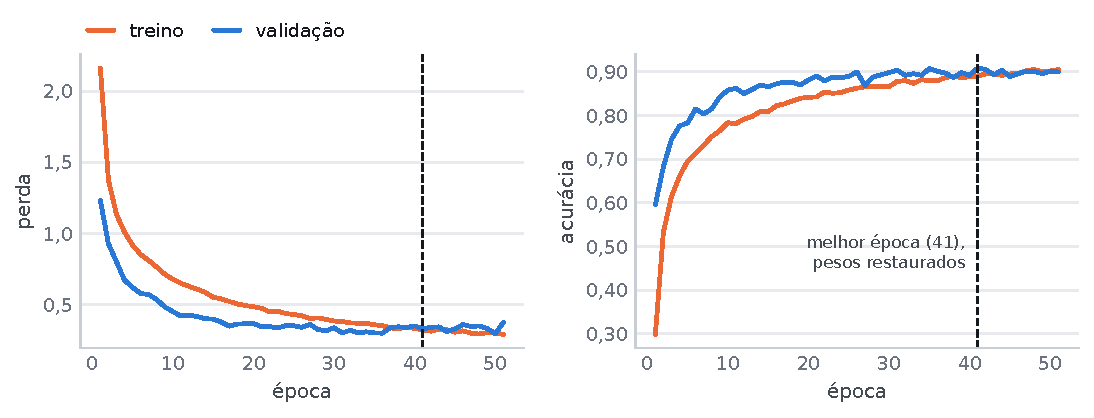
\includegraphics[width=\textwidth]{assets/resultados/curvas_treino.pdf}
    \captionsetup{justification=raggedright}
    \caption*{Fonte: Elaborada pelo autor. A linha tracejada marca a melhor época}
    \label{fig:curvasTreino}
\end{figure}

\begin{table}[H]
    \centering
    \caption{Divisão dos dados e tamanho da rede por cena}
    \footnotesize
    \setlength{\tabcolsep}{4pt}
    \begin{tabular}{|l|c|c|c|C{1.25cm}|c|c|C{1.3cm}|c|}
        \hline
        \rowcolor[HTML]{C0C0C0}
        \textbf{Cena} & \textbf{Rotulados} & \textbf{Classes} & \textbf{Treino} & \textbf{Treino (10\%)} & \textbf{Validação} & \textbf{Teste} & \textbf{Comp. do PCA} & \textbf{Parâmetros} \\
        \hline
        Indian Pines & 10.249 & 16 & 8.711 & 871 & 769 & 769 & 30 & 160.912 \\ \hline
        University of Pavia & 42.776 & 9 & 36.359 & 3.635 & 3.209 & 3.208 & 15 & 37.577 \\ \hline
        Salinas Valley & 54.129 & 16 & 46.009 & 4.602 & 4.060 & 4.060 & 15 & 38.032 \\ \hline
    \end{tabular}
    \captionsetup{justification=raggedright}
    \caption*{Fonte: Elaborada pelo autor. Divisão com a semente 42; o treino de 10\% é sorteado por classe dentro do treino completo}
    \label{tab:dadosCenas}
\end{table}

\begin{table}[H]
    \centering
    \caption{Acurácia por classe em Indian Pines com a configuração original (semente 42, treino completo)}
    \begin{tabular}{|r|l|c|c|c|}
        \hline
        \rowcolor[HTML]{C0C0C0}
        \textbf{Nº} & \textbf{Classe} & \textbf{Pixels} & \textbf{Amostras de teste} & \textbf{Acurácia} \\
        \hline
        1 & \textit{Alfalfa} & 46 & 3 & 0,0000 \\ \hline
        2 & \textit{Corn-notill} & 1.428 & 107 & 0,8692 \\ \hline
        3 & \textit{Corn-mintill} & 830 & 62 & 0,7419 \\ \hline
        4 & \textit{Corn} & 237 & 18 & 0,7778 \\ \hline
        5 & \textit{Grass-pasture} & 483 & 36 & 0,8611 \\ \hline
        6 & \textit{Grass-trees} & 730 & 55 & 1,0000 \\ \hline
        7 & \textit{Grass-pasture-mowed} & 28 & 2 & 1,0000 \\ \hline
        8 & \textit{Hay-windrowed} & 478 & 36 & 1,0000 \\ \hline
        9 & \textit{Oats} & 20 & 2 & 0,5000 \\ \hline
        10 & \textit{Soybean-notill} & 972 & 73 & 0,8767 \\ \hline
        11 & \textit{Soybean-mintill} & 2.455 & 184 & 0,9457 \\ \hline
        12 & \textit{Soybean-clean} & 593 & 44 & 0,8182 \\ \hline
        13 & \textit{Wheat} & 205 & 16 & 1,0000 \\ \hline
        14 & \textit{Woods} & 1.265 & 95 & 1,0000 \\ \hline
        15 & \textit{Buildings-Grass-Trees-Drives} & 386 & 29 & 0,9310 \\ \hline
        16 & \textit{Stone-Steel-Towers} & 93 & 7 & 0,8571 \\ \hline
         & \textbf{Média (AA)} & 10.249 & 769 & 0,8237 \\ \hline
    \end{tabular}
    \captionsetup{justification=raggedright}
    \caption*{Fonte: Elaborada pelo autor. Nomes das classes como distribuídos com a cena}
    \label{tab:porClasse}
\end{table}

\begin{figure}[H]
    \centering
    \captionsetup{justification=centering}
    \caption{Matriz de confusão do teste em Indian Pines, com a configuração original (semente 42)}
    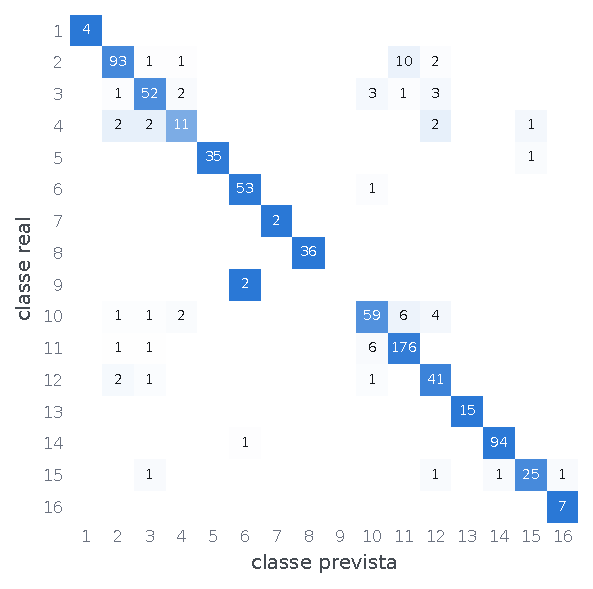
\includegraphics[width=0.72\textwidth]{assets/resultados/matriz_confusao.pdf}
    \captionsetup{justification=raggedright}
    \caption*{Fonte: Elaborada pelo autor. Cada célula traz o número de amostras; a cor, a fração da classe real. Classes numeradas como na \autoref{tab:porClasse}}
    \label{fig:matrizConfusao}
\end{figure}

\section{Organização do Código}

\begin{table}[H]
    \centering
    \caption{Pixels com rótulo diferente entre chamadas do LSC com a mesma imagem e os mesmos parâmetros}
    \begin{tabular}{|l|c|c|c|}
        \hline
        \rowcolor[HTML]{C0C0C0}
        \textbf{Cena} & \textbf{Threads do OpenCV} & \textbf{Pixels diferentes} & \textbf{Fração da cena} \\
        \hline
        Indian Pines & 32 & 401 a 623 & 1,91\% a 2,96\% \\ \hline
         & 1 & 0 & 0 \\ \hline
        University of Pavia & 32 & 222 a 556 & 0,11\% a 0,27\% \\ \hline
         & 1 & 0 & 0 \\ \hline
    \end{tabular}
    \captionsetup{justification=raggedright}
    \caption*{Fonte: Elaborada pelo autor. Catorze chamadas, em duas passadas de 7, comparadas com a primeira chamada de cada passada, com os parâmetros padrão do LSC (\autoref{qua:paramSeg}), na mesma sessão dos tempos da \autoref{tab:estruturaSeg}; a cena tem 21.025 pixels em Indian Pines e 207.400 em University of Pavia}
    \label{tab:lsc}
\end{table}

\begin{table}[H]
    \centering
    \caption{Memória retida por \textit{trial} da busca e projeção para uma campanha de 180 \textit{trials} sem liberação}
    \begin{tabular}{|l|c|c|}
        \hline
        \rowcolor[HTML]{C0C0C0}
        \textbf{Cena} & \textbf{Por \textit{trial} (MB)} & \textbf{180 \textit{trials} retidos (MB)} \\
        \hline
        Indian Pines & 2,5 & 450 \\ \hline
        University of Pavia & 5,1 & 918 \\ \hline
        Salinas Valley & 6,5 & 1.170 \\ \hline
    \end{tabular}
    \captionsetup{justification=raggedright}
    \caption*{Fonte: Elaborada pelo autor. Com a liberação, a memória do processo cresceu 16 MB numa campanha de 180 \textit{trials} em Indian Pines}
    \label{tab:memoria}
\end{table}

\section{Paralelismo}

\begin{table}[H]
    \centering
    \caption{Treino com as threads internas do PyTorch (Indian Pines, 25 épocas, CPU)}
    \begin{tabular}{|c|c|c|}
        \hline
        \rowcolor[HTML]{C0C0C0}
        \textbf{Threads} & \textbf{Tempo (s)} & \textbf{\textit{Speedup} sobre 1 thread} \\
        \hline
        1 & 8,55 & 1,00$\times$ \\ \hline
        2 & 8,45 & 1,01$\times$ \\ \hline
        4 & 7,90 & 1,08$\times$ \\ \hline
        8 & 7,81 & 1,09$\times$ \\ \hline
        16 & 11,67 & 0,73$\times$ \\ \hline
    \end{tabular}
    \captionsetup{justification=raggedright}
    \caption*{Fonte: Elaborada pelo autor. Medição avulsa}
    \label{tab:threadsTorch}
\end{table}

\begin{table}[H]
    \centering
    \caption{Quatro tarefas em sequência e em quatro threads, com e sem o GIL}
    \begin{tabular}{|l|c|c|c|}
        \hline
        \rowcolor[HTML]{C0C0C0}
        \textbf{Tarefa} & \textbf{Sequencial (s)} & \textbf{4 threads (s)} & \textbf{\textit{Speedup}} \\
        \hline
        Laço em Python puro & 1,01 & 0,91 & 1,11$\times$ \\ \hline
        Multiplicação de matrizes (código nativo) & 0,80 & 0,28 & 2,86$\times$ \\ \hline
    \end{tabular}
    \captionsetup{justification=raggedright}
    \caption*{Fonte: Elaborada pelo autor. Medição avulsa}
    \label{tab:gil}
\end{table}

\begin{table}[H]
    \centering
    \caption{Tempo do bloco paralelo da partição da cena, em segundos, e custo de partida dos processos (Indian Pines, modo independente)}
    \small
    \setlength{\tabcolsep}{3pt}
    \begin{tabular}{|c|c|c|C{1.45cm}|C{1.5cm}|c|C{1.5cm}|c|}
        \hline
        \rowcolor[HTML]{C0C0C0}
        \textbf{$N$} & \textbf{Sequencial} & \textbf{Threads} & \textbf{Proc., frio} & \textbf{Proc., quente} & \textbf{Partida} & \textbf{Partida / frio} & \textbf{Aquecimento} \\
        \hline
        2 & 13,58 & 8,45 & 11,08 & 7,31 & 3,77 & 34\% & 3,18 \\ \hline
        4 & 12,96 & 21,39 & 9,12 & 4,51 & 4,61 & 51\% & 3,91 \\ \hline
        8 & 12,29 & 54,14 & 9,01 & 3,34 & 5,67 & 63\% & 4,79 \\ \hline
        16 & 12,81 & 56,59 & 12,95 & 2,86 & 10,09 & 78\% & 7,79 \\ \hline
    \end{tabular}
    \captionsetup{justification=raggedright}
    \caption*{Fonte: Elaborada pelo autor. Médias de 3 repetições com pool quente e 2 com pool frio. Sequencial e threads com pool quente; o \textit{speedup} do pool frio na \autoref{tab:poolQuente} usa a execução sequencial correspondente, de 12,34 s a 13,55 s. Partida: tempo do pool frio menos o do pool quente}
    \label{tab:poolTempos}
\end{table}

\begin{table}[H]
    \centering
    \caption{Acurácia e tempo de uma partição no modo independente (Indian Pines, 25 épocas, lote 64, semente 42)}
    \small
    \setlength{\tabcolsep}{3pt}
    \begin{tabular}{|c|C{1.6cm}|C{1.9cm}|C{2.5cm}|C{1.9cm}|C{2.1cm}|C{1.2cm}|}
        \hline
        \rowcolor[HTML]{C0C0C0}
        \textbf{$N$} & \textbf{Treino por partição} & \textbf{OA, seq. e processos} & \textbf{OA, threads (mín.--máx.)} & \textbf{Partição sozinha (s)} & \textbf{Partição em processos (s)} & \textbf{Razão} \\
        \hline
        2 & 4.355 & 0,9090 & 0,9012--0,9103 & 6,79 & 7,24 & 1,07 \\ \hline
        4 & 2.177 & 0,9155 & 0,9116--0,9207 & 3,24 & 4,45 & 1,37 \\ \hline
        8 & 1.088 & 0,9064 & 0,8999--0,9194 & 1,54 & 3,15 & 2,05 \\ \hline
        16 & 544 & 0,8999 & 0,8921--0,9038 & 0,80 & 2,65 & 3,30 \\ \hline
        32 & 272 & 0,8505 & 0,8296--0,8648 & 0,41 & --- & --- \\ \hline
    \end{tabular}
    \captionsetup{justification=raggedright}
    \caption*{Fonte: Elaborada pelo autor. Treino por partição: média de amostras de treino em cada partição. Partição sozinha: tempo médio de uma partição na execução sequencial; em processos: com as $N$ executando juntas, no pool quente. Com $N$ = 32, só a execução sequencial, porque o pool de processos foi recusado por memória. No modo replicado, a OA foi 0,8830 em todas as execuções}
    \label{tab:particaoOA}
\end{table}

\begin{table}[H]
    \centering
    \caption{Conferência e tempos de referência da fusão concorrente, por cena}
    \small
    \setlength{\tabcolsep}{3pt}
    \begin{tabular}{|l|c|c|C{1.6cm}|C{1.3cm}|C{1.5cm}|C{1.6cm}|C{2.0cm}|}
        \hline
        \rowcolor[HTML]{C0C0C0}
        \textbf{Cena} & \textbf{Posições} & \textbf{Execuções} & \textbf{Ids e classes iguais} & \textbf{OA de teste} & \textbf{Lote, 1 thread (s)} & \textbf{Lote, 16 threads (s)} & \textbf{\mbox{Segmentação} (s)} \\
        \hline
        Indian Pines & 10.249 & 283 & 283 & 0,9051 & 0,330 & 0,196 & 0,111 \\ \hline
        University of Pavia & 42.776 & 220 & 220 & 0,9772 & 1,050 & 0,876 & 0,869 \\ \hline
        Salinas Valley & 54.129 & 220 & 220 & 0,9938 & 1,000 & 0,742 & 0,670 \\ \hline
    \end{tabular}
    \captionsetup{justification=raggedright}
    \caption*{Fonte: Elaborada pelo autor. Execuções: todas as do experimento 14 na cena, incluindo lote e sequencial. Segmentação: ramo espacial executado por T0 (PCA de 3 componentes, composição RGB e SEEDS), média nas execuções sequenciais por blocos}
    \label{tab:fusaoConferencia}
\end{table}

\begin{table}[H]
    \centering
    \caption{Posições cujas convoluções terminaram antes da publicação do mapa, em porcentagem, por número de threads de trabalho}
    \small
    \setlength{\tabcolsep}{3pt}
    \begin{tabular}{|l|l|c|c|c|c|c|c|}
        \hline
        \rowcolor[HTML]{C0C0C0}
        \textbf{Cena} & \textbf{Forma} & \textbf{Bloco} & \textbf{$N$ = 1} & \textbf{$N$ = 2} & \textbf{$N$ = 4} & \textbf{$N$ = 8} & \textbf{$N$ = 16} \\
        \hline
        Indian Pines & como no esquema & 1 & 0,0 & 0,0 & 0,0 & 0,1 & 0,2 \\ \cline{3-8}
         &  & 64 & 0,6 & 1,2 & 2,5 & 5,0 & 10,0 \\ \cline{3-8}
         &  & 1.024 & 10,0 & 20,0 & 40,0 & 79,9 & 100,0 \\ \cline{2-8}
         & desacoplada & 1 & 10,8 & 9,2 & 8,6 & 5,4 & 3,8 \\ \cline{3-8}
         &  & 64 & 94,9 & 100,0 & 100,0 & 100,0 & 100,0 \\ \cline{3-8}
         &  & 1.024 & 94,0 & 100,0 & 100,0 & 100,0 & 100,0 \\ \hline
        University of Pavia & como no esquema & 64 & 0,1 & 0,3 & 0,6 & 1,2 & 2,4 \\ \cline{3-8}
         &  & 1.024 & 2,4 & 4,8 & 9,6 & 19,2 & 38,3 \\ \cline{2-8}
         & desacoplada & 64 e 1.024 & 100,0 & 100,0 & 100,0 & 100,0 & 100,0 \\ \hline
        Salinas Valley & como no esquema & 64 & 0,1 & 0,2 & 0,5 & 0,9 & 1,9 \\ \cline{3-8}
         &  & 1.024 & 1,9 & 3,8 & 7,6 & 15,1 & 30,3 \\ \cline{2-8}
         & desacoplada & 64 e 1.024 & 100,0 & 100,0 & 100,0 & 100,0 & 100,0 \\ \hline
    \end{tabular}
    \captionsetup{justification=raggedright}
    \caption*{Fonte: Elaborada pelo autor. Médias das repetições, com a seção crítica nas duas extensões}
    \label{tab:fusaoSobreposicao}
\end{table}

\begin{table}[H]
    \centering
    \caption{Tempo de parede da fusão concorrente com a seção crítica como no esquema e mínima, em segundos (blocos de 1.024 posições)}
    \footnotesize
    \setlength{\tabcolsep}{3pt}
    \begin{tabular}{|c|c|c|c|c|c|c|}
        \hline
        \rowcolor[HTML]{C0C0C0}
        \multirow{2}{*}{\textbf{$N$}} & \multicolumn{2}{c|}{\textbf{Indian Pines}} & \multicolumn{2}{c|}{\textbf{University of Pavia}} & \multicolumn{2}{c|}{\textbf{Salinas Valley}} \\
        \cline{2-7}
        \rowcolor[HTML]{C0C0C0}
        & \textbf{Esquema} & \textbf{Mínima} & \textbf{Esquema} & \textbf{Mínima} & \textbf{Esquema} & \textbf{Mínima} \\
        \hline
        1 & 0,274 $\pm$ 0,036 & 0,304 $\pm$ 0,064 & 1,006 $\pm$ 0,090 & 1,053 $\pm$ 0,093 & 0,782 $\pm$ 0,024 & 0,869 $\pm$ 0,133 \\ \hline
        2 & 0,201 $\pm$ 0,007 & 0,279 $\pm$ 0,065 & 0,885 $\pm$ 0,054 & 0,905 $\pm$ 0,053 & 0,706 $\pm$ 0,025 & 0,713 $\pm$ 0,049 \\ \hline
        4 & 0,342 $\pm$ 0,016 & 0,363 $\pm$ 0,071 & 0,869 $\pm$ 0,079 & 0,895 $\pm$ 0,068 & 0,705 $\pm$ 0,056 & 0,688 $\pm$ 0,038 \\ \hline
        8 & 0,164 $\pm$ 0,008 & 0,191 $\pm$ 0,036 & 0,948 $\pm$ 0,085 & 0,975 $\pm$ 0,085 & 0,666 $\pm$ 0,014 & 0,687 $\pm$ 0,036 \\ \hline
        16 & 0,171 $\pm$ 0,006 & 0,173 $\pm$ 0,011 & 0,983 $\pm$ 0,086 & 0,986 $\pm$ 0,101 & 0,692 $\pm$ 0,045 & 0,692 $\pm$ 0,047 \\ \hline
    \end{tabular}
    \captionsetup{justification=raggedright}
    \caption*{Fonte: Elaborada pelo autor. Forma como no esquema; média e desvio de 5 repetições}
    \label{tab:fusaoSecao}
\end{table}

\section{Automação de Hiperparâmetros}

\begin{table}[H]
    \centering
    \caption{Diferença entre a melhor e a pior estratégia de busca, por orçamento de épocas (Indian Pines, 3 sementes)}
    \begin{tabular}{|c|l|l|c|c|l|}
        \hline
        \rowcolor[HTML]{C0C0C0}
        \textbf{Orçamento} & \textbf{Melhor} & \textbf{Pior} & \textbf{Diferença (pp)} & \textbf{Desvio comb. (pp)} & \textbf{Leitura} \\
        \hline
        10 épocas & Genética & Aleatória & 1,60 & 2,01 & ruído \\ \hline
        40 épocas & Genética & Aleatória & 2,56 & 1,93 & ruído \\ \hline
        200 épocas & Genética & Aleatória & 2,21 & 3,77 & ruído \\ \hline
    \end{tabular}
    \captionsetup{justification=raggedright}
    \caption*{Fonte: Elaborada pelo autor. Melhor validação de cada busca, média de 3 sementes (\autoref{tab:estrategias}); afirmável quando a diferença excede duas vezes o desvio combinado}
    \label{tab:estrategiasRuido}
\end{table}

\begin{table}[H]
    \centering
    \caption{Como cada estratégia gastou os 20 \textit{trials} (Indian Pines, médias de 3 sementes)}
    \small
    \setlength{\tabcolsep}{3pt}
    \begin{tabular}{|c|l|C{1.8cm}|C{1.8cm}|C{1.8cm}|C{1.8cm}|}
        \hline
        \rowcolor[HTML]{C0C0C0}
        \textbf{Orçamento} & \textbf{Estratégia} & \textbf{\textit{Trial} do melhor} & \textbf{Épocas por \textit{trial}} & \textbf{Treino da busca (s)} & \textbf{\textit{Trials} com SEEDS} \\
        \hline
        10 épocas & Aleatória & 14,0 & 8,7 & 10,1 & 30\% \\
        & TPE & 11,0 & 9,7 & 11,2 & 53\% \\
        & Genética & 13,0 & 9,5 & 10,3 & 55\% \\ \hline
        40 épocas & Aleatória & 6,7 & 36,2 & 38,5 & 30\% \\
        & TPE & 6,7 & 35,8 & 32,4 & 33\% \\
        & Genética & 16,0 & 36,9 & 33,2 & 38\% \\ \hline
        200 épocas & Aleatória & 11,3 & 66,9 & 65,0 & 30\% \\
        & TPE & 18,7 & 67,9 & 64,1 & 33\% \\
        & Genética & 10,7 & 77,8 & 64,7 & 33\% \\ \hline
    \end{tabular}
    \captionsetup{justification=raggedright}
    \caption*{Fonte: Elaborada pelo autor. \textit{Trial} do melhor: posição, entre os 20, do \textit{trial} de maior validação. Épocas por \textit{trial}: épocas efetivamente treinadas, abaixo do teto quando a parada antecipada atua}
    \label{tab:estrategiasCusto}
\end{table}

\begin{table}[H]
    \centering
    \caption{Acurácia de validação média por valor de cada hiperparâmetro (540 \textit{trials} do experimento 08, Indian Pines)}
    \begin{tabular}{|l|l|c|c|c|}
        \hline
        \rowcolor[HTML]{C0C0C0}
        \textbf{Hiperparâmetro} & \textbf{Valor} & \textbf{Validação média} & \textbf{\textit{Trials}} & \textbf{Amplitude (pp)} \\
        \hline
        \multirow{3}{*}{Dropout} & 0,20 & 0,6927 & 220 & \multirow{3}{*}{18,10} \\ \cline{2-4}
         & 0,35 & 0,6368 & 194 &  \\ \cline{2-4}
         & \textbf{0,50} & 0,5117 & 126 &  \\ \hline
        \multirow{3}{*}{Taxa de aprendizado} & 0,0003 & 0,5162 & 120 & \multirow{3}{*}{15,26} \\ \cline{2-4}
         & \textbf{0,001} & 0,6592 & 254 &  \\ \cline{2-4}
         & 0,003 & 0,6688 & 166 &  \\ \hline
        \multirow{4}{*}{Segmentador} & \textbf{SEEDS} & 0,6925 & 202 & \multirow{4}{*}{14,89} \\ \cline{2-4}
         & SLIC & 0,5436 & 90 &  \\ \cline{2-4}
         & LSC & 0,6356 & 148 &  \\ \cline{2-4}
         & Watershed & 0,5752 & 100 &  \\ \hline
        \multirow{3}{*}{Componentes do PCA} & 15 & 0,5750 & 153 & \multirow{3}{*}{8,35} \\ \cline{2-4}
         & \textbf{30} & 0,6585 & 174 &  \\ \cline{2-4}
         & 45 & 0,6472 & 213 &  \\ \hline
        \multirow{3}{*}{\textit{Weight decay}} & \textbf{0} & 0,6497 & 196 & \multirow{3}{*}{4,55} \\ \cline{2-4}
         & $10^{-5}$ & 0,6339 & 176 &  \\ \cline{2-4}
         & $10^{-4}$ & 0,6042 & 168 &  \\ \hline
        \multirow{3}{*}{Tamanho do lote} & \textbf{32} & 0,6186 & 160 & \multirow{3}{*}{1,81} \\ \cline{2-4}
         & 64 & 0,6343 & 221 &  \\ \cline{2-4}
         & 128 & 0,6367 & 159 &  \\ \hline
    \end{tabular}
    \captionsetup{justification=raggedright}
    \caption*{Fonte: Elaborada pelo autor. Em negrito, o valor da configuração original. Amplitude: diferença entre o melhor e o pior valor do hiperparâmetro}
    \label{tab:eixos}
\end{table}

\begin{table}[H]
    \centering
    \caption{Configuração original contra configuração otimizada em AA, Kappa e épocas treinadas (Indian Pines, 5 sementes, 10\% do treino)}
    \small
    \setlength{\tabcolsep}{3pt}
    \begin{tabular}{|l|l|c|c|C{1.3cm}|C{1.3cm}|l|}
        \hline
        \rowcolor[HTML]{C0C0C0}
        \textbf{Segmentador} & \textbf{Métrica} & \textbf{Original} & \textbf{Otimizada} & \textbf{Ganho (pp)} & \textbf{Limiar (pp)} & \textbf{Leitura} \\
        \hline
        \multirow{3}{*}{SEEDS} & AA & 0,5903 $\pm$ 0,0307 & 0,6985 $\pm$ 0,0443 & +10,81 & 10,78 & afirmável \\ \cline{2-7}
         & Kappa & 0,7058 $\pm$ 0,0203 & 0,7910 $\pm$ 0,0131 & +8,52 & 4,83 & afirmável \\ \cline{2-7}
         & Épocas & 53,0 & 80,4 &  &  &  \\ \hline
        \multirow{3}{*}{SLIC} & AA & 0,4071 $\pm$ 0,1550 & 0,4835 $\pm$ 0,1707 & +7,64 & 46,12 & ruído \\ \cline{2-7}
         & Kappa & 0,5342 $\pm$ 0,2087 & 0,5839 $\pm$ 0,2211 & +4,97 & 60,81 & ruído \\ \cline{2-7}
         & Épocas & 71,0 & 115,4 &  &  &  \\ \hline
        \multirow{3}{*}{LSC} & AA & 0,4343 $\pm$ 0,0501 & 0,6104 $\pm$ 0,0298 & +17,61 & 11,67 & afirmável \\ \cline{2-7}
         & Kappa & 0,6294 $\pm$ 0,0469 & 0,7310 $\pm$ 0,0256 & +10,16 & 10,69 & ruído \\ \cline{2-7}
         & Épocas & 73,0 & 64,6 &  &  &  \\ \hline
        \multirow{3}{*}{Watershed} & AA & 0,3847 $\pm$ 0,1534 & 0,4224 $\pm$ 0,2582 & +3,77 & 60,07 & ruído \\ \cline{2-7}
         & Kappa & 0,5056 $\pm$ 0,2118 & 0,4777 $\pm$ 0,2847 & $-$2,79 & 70,98 & ruído \\ \cline{2-7}
         & Épocas & 82,2 & 72,4 &  &  &  \\ \hline
    \end{tabular}
    \captionsetup{justification=raggedright}
    \caption*{Fonte: Elaborada pelo autor. Limiar: duas vezes o desvio combinado das duas configurações. Épocas: média das épocas treinadas até a parada}
    \label{tab:impactoHPOCompleto}
\end{table}

\section{Segmentadores}

\begin{table}[H]
    \centering
    \caption{AA, Kappa e diferença de OA para o SEEDS sob otimização conjunta (5 sementes, 10\% do treino)}
    \footnotesize
    \setlength{\tabcolsep}{3pt}
    \begin{tabular}{|l|l|c|c|C{1.4cm}|C{1.2cm}|l|}
        \hline
        \rowcolor[HTML]{C0C0C0}
        \textbf{Cena} & \textbf{Segmentador} & \textbf{AA} & \textbf{Kappa} & \textbf{Dif. de OA (pp)} & \textbf{Limiar (pp)} & \textbf{Leitura} \\
        \hline
        \multirow{4}{*}{Indian Pines} & SEEDS & 0,6985 $\pm$ 0,0443 & 0,7910 $\pm$ 0,0131 & --- & --- & referência \\ \cline{2-7}
         & SLIC & 0,4835 $\pm$ 0,1707 & 0,5839 $\pm$ 0,2211 & $-$17,63 & 37,19 & ruído \\ \cline{2-7}
         & LSC & 0,6104 $\pm$ 0,0298 & 0,7310 $\pm$ 0,0256 & $-$5,18 & 4,95 & afirmável \\ \cline{2-7}
         & Watershed & 0,4224 $\pm$ 0,2582 & 0,4777 $\pm$ 0,2847 & $-$25,28 & 45,15 & ruído \\ \hline
        \multirow{4}{*}{University of Pavia} & SEEDS & 0,9323 $\pm$ 0,0116 & 0,9358 $\pm$ 0,0055 & --- & --- & referência \\ \cline{2-7}
         & SLIC & 0,9249 $\pm$ 0,0092 & 0,9381 $\pm$ 0,0051 & +0,19 & 1,14 & ruído \\ \cline{2-7}
         & LSC & 0,7422 $\pm$ 0,3156 & 0,7283 $\pm$ 0,3642 & $-$11,82 & 39,73 & ruído \\ \cline{2-7}
         & Watershed & 0,9394 $\pm$ 0,0122 & 0,9410 $\pm$ 0,0026 & +0,41 & 0,93 & ruído \\ \hline
        \multirow{4}{*}{Salinas Valley} & SEEDS & 0,9497 $\pm$ 0,0155 & 0,9590 $\pm$ 0,0084 & --- & --- & referência \\ \cline{2-7}
         & SLIC & 0,9122 $\pm$ 0,0060 & 0,9445 $\pm$ 0,0050 & $-$1,31 & 1,76 & ruído \\ \cline{2-7}
         & LSC & 0,9493 $\pm$ 0,0098 & 0,9453 $\pm$ 0,0060 & $-$1,23 & 1,86 & ruído \\ \cline{2-7}
         & Watershed & 0,9321 $\pm$ 0,0183 & 0,9440 $\pm$ 0,0052 & $-$1,35 & 1,77 & ruído \\ \hline
    \end{tabular}
    \captionsetup{justification=raggedright}
    \caption*{Fonte: Elaborada pelo autor. Limiar: duas vezes o desvio combinado do segmentador e do SEEDS. Em University of Pavia, o LSC colapsou em uma das cinco sementes}
    \label{tab:segmentadoresCompleto}
\end{table}

\chapter{Desvios em Relação ao Projeto}
\label{ap:desvios}

O \autoref{qua:desvios} reúne os desvios da implementação, e o \autoref{qua:desviosExperimentos}, os da campanha experimental, cada um com o seu motivo, em relação ao projeto do \autoref{cap:proj}.

\begin{quadro}[H]
    \centering
    \small
    \caption{Desvios em relação ao projeto: implementação}
    \begin{tabular}{|>{\RaggedRight\arraybackslash}p{0.27\textwidth}|>{\RaggedRight\arraybackslash}p{0.27\textwidth}|>{\RaggedRight\arraybackslash}p{0.36\textwidth}|}
        \hline
        \rowcolor[HTML]{C0C0C0}
        \textbf{Previsto} & \textbf{Realizado} & \textbf{Motivo} \\
        \hline
        TensorFlow/Keras ou PyTorch & PyTorch & Arquitetura, PCA, divisão dos dados e hiperparâmetros de treino do original preservados em PyTorch, com execução determinística; a regra de parada antecipada foi trocada (última linha deste quadro) \\
        \hline
        CNN com 16, 32, 64 e 128 filtros, \textit{max-pooling} e \textit{softmax} & 16, 32, 64 e 64 filtros, sem \textit{pooling}, saída em \textit{logits} & A arquitetura do notebook original, que é a referência; o \textit{softmax} é aplicado pela função de perda \\
        \hline
        Rótulo do superpixel codificado em \textit{one-hot} & Identificador numérico concatenado, como no original & A configuração original é a referência; o \textit{embedding} foi implementado para análise \\
        \hline
        Critério do RF03: classificação com fusão superior à puramente espectral & Fusão verificada pela concatenação e pela dimensão da entrada da cabeça densa (1.025 em Indian Pines); a vantagem sobre a rede puramente espectral é a reportada por \citeonline{Souza2023} & A fusão faz parte da configuração de referência e não é variável de estudo; nenhuma configuração sem fusão é treinada \\
        \hline
        SEEDS, LSC e Watershed & SEEDS, SLIC, LSC e Watershed & O SLIC é uma referência frequente nas avaliações de algoritmos de superpixels \cite{Stutz2018} e uma comparação natural \\
        \hline
        Busca em grade e Otimização Bayesiana com Ray Tune & Busca aleatória, TPE (Optuna) e algoritmo genético & As 2.916 combinações custariam 146 vezes uma busca de 20 \textit{trials}; o TPE aceita diretamente o segmentador, que é categórico; o genético acrescenta uma estratégia populacional (\autoref{sec:desHPO}) \\
        \hline
        Épocas, filtros, tamanho dos \textit{kernels} e otimizador entre os hiperparâmetros da CNN & Taxa de aprendizado, \textit{dropout}, \textit{weight decay} e lote; arquitetura e otimizador Adam fixos & A arquitetura e o otimizador são os do original, que é a referência; o orçamento de épocas foi estudado à parte, no experimento 08 \\
        \hline
        Google Colab ou HPC & GPU local (RTX 5070 Laptop) & Suficiente para as três cenas, com controle total do ambiente; os 15,8 GB de RAM impediram o pool de 32 processos (\autoref{sec:resParalelismo}) \\
        \hline
        Parada do notebook original: perda de validação, paciência 5 & Acurácia de validação, paciência 10, melhores pesos restaurados; meta de 0,95 nos experimentos de segmentadores e de hiperparâmetros & A mesma métrica governa a parada e a seleção \\
        \hline
    \end{tabular}
    \captionsetup{justification=raggedright}
    \caption*{Fonte: Elaborado pelo autor}
    \label{qua:desvios}
\end{quadro}

\begin{quadro}[H]
    \centering
    \small
    \caption{Desvios em relação ao projeto: campanha experimental}
    \begin{tabular}{|>{\RaggedRight\arraybackslash}p{0.27\textwidth}|>{\RaggedRight\arraybackslash}p{0.27\textwidth}|>{\RaggedRight\arraybackslash}p{0.36\textwidth}|}
        \hline
        \rowcolor[HTML]{C0C0C0}
        \textbf{Previsto} & \textbf{Realizado} & \textbf{Motivo} \\
        \hline
        Segmentadores com CNN fixa & Segmentadores sob otimização conjunta & O desenho com CNN fixa se mostrou inválido (\autoref{cap:resultados}) \\
        \hline
        85\% das amostras para treino & 10\% desse treino nos experimentos de segmentadores e de hiperparâmetros & Cada execução fica cerca de 5,7 vezes mais barata em Indian Pines (\autoref{tab:fracaoTreino}), o que viabilizou os 540 \textit{trials} do experimento 08; validação e teste permanecem inteiros \\
        \hline
        Todos os experimentos nas três cenas & CNN fixa (05) em Indian Pines e University of Pavia; segmentadores (06) e fusão concorrente (14) nas três; busca (08), ganho da busca de hiperparâmetros (10) e partição (11 e 13) em Indian Pines & Custo de tempo; Indian Pines é a cena de menor acurácia na linha de base (OA 0,9051; \autoref{tab:linhaBase}) \\
        \hline
        Testes de significância estatística & Diferença afirmável quando excede duas vezes o desvio combinado das duas condições entre sementes & Com 3 a 5 sementes por condição, um critério simples e explícito; por usar o desvio das execuções, e não o erro padrão da média, é mais exigente que o mesmo limiar aplicado ao erro padrão; o pareamento por semente não foi explorado \\
        \hline
        Segmentação em processo e CNN na GPU, em paralelo & Threads e processos em CPU, em três níveis & Em Indian Pines, o pré-processamento é 0,9\% de uma execução e a inferência, 0,4\% (\autoref{sec:resParalelismo}); o tempo concentra-se no treino, e a comparação entre executores exige o mesmo dispositivo \\
        \hline
        Paralelização sobre a melhor configuração identificada & Fusão concorrente sobre a configuração original; partição com lote 64 e 25 épocas & Interessa o tempo entre executores, com a mesma configuração dos dois lados \\
        \hline
    \end{tabular}
    \captionsetup{justification=raggedright}
    \caption*{Fonte: Elaborado pelo autor}
    \label{qua:desviosExperimentos}
\end{quadro}

\end{apendicesenv}

\end{document}
